\documentclass[a4paper, 12pt]{report}

%%%%%%%%%%%%
% Packages %
%%%%%%%%%%%%

\usepackage[english]{babel}
\usepackage[noheader]{packages/sleek}
\usepackage{packages/sleek-title}
\usepackage{packages/sleek-theorems}
\usepackage{packages/sleek-listings}
\usepackage[explicit]{titlesec}
\usepackage{tikz}
\usepackage{lipsum}
\usepackage{amsfonts}
\usepackage{amsmath}
\usepackage{amssymb}
\usepackage{graphicx}
\usepackage{graphbox}
\usepackage{bm}
\usepackage{cancel}
\usepackage{color}
\usepackage{mathrsfs}
\usepackage{tikz}
\usepackage{simpler-wick}
\usepackage[mathscr]{euscript}

%%%%%%%%%%%%%%
% Title-page %
%%%%%%%%%%%%%%

\title{Notes on Quantum Field Theory}
\author{\textit{Jie Ren}}
\date{\today}

%%%%%%%%%%
% Others %
%%%%%%%%%%

\def\tbs{\textbackslash}
\FrameTBStyle{mathematica}
%%%%%%%%%%%%
% Document %
%%%%%%%%%%%%

\begin{document}
\maketitle
\romantableofcontents

\chapter{Relativistic Quantum Field Theory}

\section{Lorentz Invariance}

\subsection{The Lorentz Algebra}
The metric is chosen to be 
\begin{equation}
	g_{\mu\nu}=g^{\mu\nu}=\mathrm{diag}(-1,+1,+1,+1).
\end{equation}
The Lorentz transformation ${\Lambda^{\mu}}_{\nu}$ satisfies
\begin{equation}
{\Lambda^{\mu}}_{\alpha}{\Lambda^{\nu}}_{\beta} g_{\mu\nu} = g_{\alpha\beta}.
\end{equation}
From this we have
\begin{equation*}
	g^{\gamma\alpha}{\Lambda^{\mu}}_{\alpha}{\Lambda^{\nu}}_{\beta} g_{\mu\nu} 
	= g^{\gamma\alpha}g_{\alpha\beta} 
	\quad \Longrightarrow \quad
	{\Lambda_{\nu}}^{\gamma}{\Lambda^{\nu}}_{\beta} 
	= {\delta^{\gamma}}_{\beta},
\end{equation*}
The inverse Lorentz transformation satisfies:
\begin{equation*}
	{(\Lambda^{-1})^{\mu}}_{\nu} = {\Lambda_{\nu}}^{\mu}.
\end{equation*}
The infinitesimal transformation is denoted as
\begin{equation*}
\begin{aligned}
	{\Lambda^{\mu}}_{\nu} &= {\delta^{\mu}}_{\nu}+\delta{\omega^{\mu}}_{\nu} \\
	{(\Lambda^{-1})^\mu}_\nu &= {\delta^{\mu}}_{\nu}-\delta{\omega^\mu}_\nu
\end{aligned}
	\quad \Longrightarrow \quad
	g_{\alpha\nu}\delta{\omega^{\nu}}_{\beta}+\delta{\omega^{\mu}}_{\alpha}g_{\mu\beta}
	=\delta\omega_{\alpha\beta} + \delta\omega_{\beta\alpha} = 0.
\end{equation*}
A representation of Lorentz group $U(\Lambda)$ can be parametrized as:
\begin{equation}
	U(\Lambda) = \exp\left(\frac{i}{2}\omega_{\mu\nu}M^{\mu\nu}\right).
\end{equation}
Another useful parametrization is
\begin{equation*}
	\theta_i \equiv \frac{1}{2}\varepsilon_{ijk}\omega_{jk}, \ 
	\beta_i \equiv \omega_{0i}.
\end{equation*}
A new set of generators are:
\begin{equation}
	J_i \equiv \frac{1}{2}\varepsilon_{ijk}M^{jk},\ 
	K_i \equiv M^{i0},
\end{equation}
where $J_i$'s are the generators of the spatial rotations, and $K_i$'s are the generators of Lorentz boosts.

In the fundamental representation, the generators are represented by
\begin{equation*}
\begin{aligned}
	J_1 &= \left[\begin{array}{cccc} 0 & & & \\ & 0 & & \\ & & 0 & -i \\ & & i & 0 \end{array}\right], & 
	J_2 &= \left[\begin{array}{cccc} 0 & & & \\ & 0 & & i \\ & & 0 & \\ & -i & & 0 \end{array}\right], &
	J_3 &= \left[\begin{array}{cccc} 0 & & & \\ & 0 & -i & \\ & i & 0 & \\ & & & 0 \end{array}\right], \\
	K_1 &= \left[\begin{array}{cccc} 0 & -i & & \\ -i & 0 & & \\ & & 0 & \\ & & & 0 \end{array}\right], & 
	K_2 &= \left[\begin{array}{cccc} 0 & & -i & \\ & 0 & & \\ -i & & 0 & \\ & & & 0 \end{array}\right], &
	K_3 &= \left[\begin{array}{cccc} 0 & & & -i \\ & 0 & & \\ & & 0 & \\ -i & & & 0 \end{array}\right].
\end{aligned}
\end{equation*}
The Lie algebra of the Lorentz algebra can be explicitly done using the fundamental representation. 
The result is
\begin{equation}
\begin{aligned}
	\left[J_i, J_j\right] &= i \varepsilon_{ijk} J_k, \\
	\left[J_i, K_j\right] &= i \varepsilon_{ijk} K_k, \\
	\left[K_i, K_j\right] &= -i\varepsilon_{ijk} J_k.
\end{aligned}
\end{equation}
By defining a new set of generators:
\begin{equation}
	N_i^{L} \equiv \frac{J_i - i K_i}{2},\ 
	N_i^{R} \equiv \frac{J_i + i K_i}{2}.
\end{equation}
They satisfies two independent $\mathfrak{su}(2)$ algebra:
\begin{equation*}
\begin{aligned}
	\left[N_i^L, N_j^L \right] &= i\varepsilon_{ijk}N_k^L, \\
	\left[N_i^R, N_j^R \right] &= i\varepsilon_{ijk}N_k^R, \\
	\left[N_i^L, N_j^R \right] &= 0.
\end{aligned}
\end{equation*}
That is, the Lorentz algebra is isomorphic to two $\mathfrak{su}(2)$ algebra,
\begin{equation}
	\mathfrak{so}(3,1) \approx \mathfrak{su}_L(2)\oplus\mathfrak{su}_R(2).
	\label{eq:Lorentz-alg-decomp}
\end{equation}
From Eq.~(\ref{eq:Lorentz-alg-decomp}), we know that the representation of the Lorentz algebra can be labelled by $j_L$ and $j_R$.
Note that the fundamental representation correspond to
\begin{equation*}
	\left(j_L=\frac{1}{2},j_R=\frac{1}{2}\right).
\end{equation*}
The specific form of the group is
\begin{equation*}
	\Lambda(\vec\theta,\vec\beta)
	=\exp\left[i(\vec\theta+i\vec\beta)\cdot \vec N^L + i(\vec\theta-i\vec\beta)\cdot \vec N^R\right].
\end{equation*}
The spinor representations are those with $j_L=1/2$ or $j_R=1/2$. 
Specifically, we define the left-hand spinor $\psi_L$ and right-hand spinor $\psi_R$ that transform as:
\begin{equation}
\begin{aligned}
	\Lambda_L(\vec\theta,\vec\beta)\psi_L 
	&= \exp\left(\frac{i}{2}\vec\theta\cdot\vec\sigma-\frac{1}{2}\vec\beta\cdot\vec\sigma \right) \psi_L, \\
	\Lambda_R(\vec\theta,\vec\beta)\psi_R 
	&= \exp\left(\frac{i}{2}\vec\theta\cdot\vec\sigma+\frac{1}{2}\vec\beta\cdot\vec\sigma \right) \psi_R.
\end{aligned}
\end{equation}
Using the fact $\sigma^2 \cdot \vec\sigma^* \cdot\sigma^2 = -\vec\sigma$, the left-hand and the right-hand representations are related by:
\begin{equation}
\begin{aligned}
	\sigma^2 \Lambda_L^* \sigma^2 &= \Lambda_R, & \sigma^2 \Lambda_L^T \sigma^2 &= \Lambda_L^{-1}, \\
	\sigma^2 \Lambda_R^* \sigma^2 &= \Lambda_L, & \sigma^2 \Lambda_R^T \sigma^2 &= \Lambda_R^{-1}.
\end{aligned}
\end{equation}
For this reason, the left-hand and right-hand spinor can be interchanged by
\begin{equation}
\begin{aligned}
	\sigma^2 \psi_L^* &\sim \chi_R, & \psi_L^\dagger \sigma^2 &\sim \chi^\dagger_R \\
	\sigma^2 \psi_R^* &\sim \chi_L, & \psi^\dagger_R \sigma^2 &\sim \chi^\dagger_L.
	\label{eq:left-right-spinor-rel}
\end{aligned}
\end{equation}



\subsection{The Invariant Symbols}
The invariant symbols can be thought as the Clebsch-Gordan coefficients that help to form singlets.
The first singlet comes from the decomposition
\begin{equation*}
	\frac{1}{2}\otimes \frac{1}{2} \approx 0 \oplus 1.
\end{equation*}
Correspondingly, we can check that for each-hand-side spinor, the quadratic forms
\begin{equation}
	\psi_L^T\sigma^2\chi_L \quad \text{or} \quad 
	\psi_R^T\sigma^2\chi_R
	\label{eq:inner-product-inv-symbol}
\end{equation}
are singlets.
We can define the first invariant symbol as\footnote{We use the dotted symbol to denote the right-hand spinor indices.}
\begin{equation}
	\varepsilon^{ab} = \varepsilon^{\dot a \dot b} = i(\sigma^2)_{ab}, \quad
	\varepsilon_{ab} = \varepsilon_{\dot a \dot b} = -i(\sigma^2)_{ab}.
\end{equation}
The symbol $\varepsilon^{ab}$ or $\varepsilon_{ab}$ also serve as the index raising/lowering symbol, i.e.,
\begin{equation}
	\varepsilon^{ab}\psi_b = \psi^a,\ 
	\varepsilon_{ab}\psi^b = \psi_a.
\end{equation}
The singlet (\ref{eq:inner-product-inv-symbol}) is then defined as the inner product of two spinors:
\begin{equation}
	\psi\cdot\chi 
	\equiv \varepsilon_{ab}\psi^a\chi^b
	= \psi^a\chi_{a}
	= -\varepsilon_{ba}\psi^a\chi^b
	= -\psi_b\chi^b.
\end{equation}
In addition, because of (\ref{eq:left-right-spinor-rel}), the expressions
\begin{equation*}
	\psi_L^\dagger \chi_R \quad \text{and} \quad \psi_R^\dagger \chi_L
\end{equation*}
are also singlets.

Besides, we know there should be another invariant symbol from the decomposition
\begin{equation*}
	\left(\frac{1}{2}, 0\right) \otimes \left(0,\frac{1}{2}\right)
	\approx \left(0, 0\right) \oplus \cdots.
\end{equation*}
For this reason, we are searching for the symbol $M$ that the expression
\begin{equation*}
	M^\mu_{a\dot b} \psi^a_L \chi^{\dot b}_R
\end{equation*}
transforms as the Lorentz vector.
The matrix $M^\mu$ should transform as
\begin{equation*}
	M^\mu \longrightarrow \Lambda_L^T \cdot M^\mu \cdot \Lambda_R = {\Lambda^\mu}_\nu M^\nu.
\end{equation*}
Use the fact that $\sigma^2 \cdot \Lambda_L^T \cdot \sigma^2 = \Lambda_L^{-1}$, the above equation transforms to
\begin{equation*}
	\left(\sigma^2 M^\mu\right) \longrightarrow \Lambda_L^{-1} \cdot \left(\sigma^2 M^\mu\right)\cdot \Lambda_R.
\end{equation*}
We then show the matrices $\sigma^\mu = (\sigma^0,\vec\sigma)$ satisfies the requirement.
Firstly, for the spatial rotation,
\begin{equation*}
	\Lambda_L(\vec\theta,\vec 0) = \Lambda_R(\theta,\vec 0) = \exp\left(i\vec\theta\cdot \frac{\vec\sigma}{2}\right)
\end{equation*}
The Pauli matrix transform as
\begin{equation*}
	\left(1-i\delta\vec\theta\cdot\frac{\vec\sigma}{2}\right)\sigma^j\left(1+i\delta\vec\theta\cdot \frac{\vec\sigma}{2}\right)
	= \sigma^j + i\delta\theta_i \left(-i \varepsilon_{ijk}\sigma^k \right)
\end{equation*}
Secondly, for the boosts,
\begin{equation*}
	\Lambda_L(\vec 0, \vec\beta) = \exp\left(-\vec\beta\cdot \frac{\vec\sigma}{2}\right),\ 
	\Lambda_R(\vec 0, \vec\beta) = \exp\left(+\vec\beta\cdot \frac{\vec\sigma}{2}\right)
\end{equation*}
The Pauli matrix transform as
\begin{equation*}
	\left(1+\delta\vec\beta\cdot\frac{\vec\sigma}{2}\right)\sigma^\mu \left(1+\delta\vec\beta\cdot \frac{\vec\sigma}{2}\right) = \begin{cases}
		 \sigma^0 + i\delta\beta_i \cdot (-i\sigma^i), & \mu = 0 \\
		 \sigma^j + i\delta\beta_j (-i\sigma^0), & \mu = j
	\end{cases}.
\end{equation*}
We thus have shown indeed that
\begin{equation}
	\psi_L^T \sigma^2 \sigma^\mu \chi_R
\end{equation}
is a Lorentz vector.
Further more, from (\ref{eq:left-right-spinor-rel}), we know that
\begin{equation}
	\eta_R^\dagger \sigma^\mu \chi_R
\end{equation}
is also a Lorentz vector.
Similarly, consider the Lorentz vector 
\begin{equation*}
	N^\mu_{\dot a b} \psi^{\dot a}_R \chi^{b}_R,
\end{equation*}
which together with $\sigma^2$ should transforms as
\begin{equation*}
	\left(\sigma^2 N^\mu\right) \longrightarrow 
	\Lambda_R^{-1} \cdot \left(\sigma^2 N^\mu\right)\cdot \Lambda_L.
\end{equation*}
We can check that $\bar\sigma^\mu = (\sigma^0,-\vec\sigma)$ satisfies the requirement, and thus 
\begin{equation}
	\eta_L^\dagger \bar\sigma^\mu \chi_L
\end{equation}
is also a Lorentz vector.


\section{Klein-Gordon Field}

In relativistic quantum field theory, the Lagrangian should be a singlet under Lorentz transformation.
Different free fields correspond to different representation of the Lorentz algebra.
The symmetry under Lorentz transformation also restrict the possible terms that can appear in the Lagrangian.


The simplest case is when $j_L=j_R = 0$, corresponding to the scalar field, which we denote as $\phi(x)$.
Since the field it self is singlet, any polynomial of the field in principle can appear in the theory.
When considering the free theory, we restrict our attention to the quadratic terms.
We require the field theory to have a dynamical term, which contains derivative the the field.
The derivative operator $\partial^\mu$ transforms as the fundamental representation.
To be Lorentz invariant, the allowed free theory can only be
\begin{equation}
	\mathcal L_{\mathrm{K-G}} = \frac{1}{2}\partial^\mu \phi \partial_\mu \phi -\frac{m^2}{2}\phi^2 
	\simeq -\frac{1}{2}\phi (\partial^2+m^2) \phi.
\end{equation}



\subsection{Path-integral Formalism}
In this note, the space-time Fourier transformation is defined as
\begin{equation}
\begin{aligned}
	\tilde{\phi}(k) &= \int d^{d}x e^{ik\cdot x} \phi(x), \\ 
	\phi(x) &= \int \frac{d^{d}k}{(2\pi)^{d}} e^{-ik\cdot x}\tilde{\phi}(k),
\end{aligned}
\end{equation}
where the inner product of two 4-momentum and 4-coordinate is
\begin{equation}
	k\cdot x=\omega t-\vec k\cdot \vec x.
\end{equation}

Consider the action for free field with source
\begin{equation}
	S_0[\phi,J]
	= \int d^dx\left[\mathcal{L}_0(\phi) + J(x)\cdot\phi(x) \right].
\end{equation}
In momentum space, the free Lagrangian (with source) is 
\begin{equation*}
	\tilde{\mathcal L}_0[\phi_k,J]=\tilde\phi(k)( k^2-m^2)\tilde\phi(-k)+\tilde J(k)\cdot\tilde\phi(-k)+\tilde\phi(k)\cdot\tilde J(-k).
\end{equation*}
In the path integral formalism, we consider the partition function 
\begin{equation}
	Z_0[J] = \int D[\phi] \exp(iS_0[\phi,J]).
\end{equation}
The partition function for free field:
\begin{eqnarray*}
	\frac{Z_0[J]}{Z_0[0]}
	&=& \exp\left(-\frac{i}{2}\int \frac{d^dk}{(2\pi)^d} \frac{\tilde J(k) \tilde J(-k)}{k^2-m^2+i\epsilon} \right) \\
	&=& \exp\left(-\frac{i}{2}\int d^dx_1 d^dx_2 J(x_1)\Delta_0(x_1-x_2)J(x_2)\right).
\end{eqnarray*}
where the propagator is
\begin{equation}
	\Delta_0(x_1-x_2) = \int \frac{d^dk}{(2\pi)^d} \frac{e^{-ik\cdot x}}{k^2-m^2+i\epsilon},
\end{equation}
where the extra $i\epsilon$ term is use to bring the singularities infinitesimally below the real axis. 
This infinitesimal value can be absorbed into the mass term, by regarding the mass term $m^2$ as $m^2-i\epsilon$.

Note that $\Delta_0(x_1-x_2)$ is related to the correlation function:
\begin{equation}
	\langle 0| T\phi(x_1)\phi(x_2)|0\rangle
	= \frac{\delta}{i\delta J(x_1)}\frac{\delta}{i\delta J(x_2)} Z_0[J] 
	= i\Delta(x_1-x_2).
\end{equation}

\begin{framedrmk}[Gaussian Integral for Real Scalar Field]
The real Gaussian integral formula is
\begin{equation}
	\int d\bm v \exp\left(-\frac{1}{2}\bm{v}^T \cdot A\cdot \bm{v} + \bm{b}^T \cdot \bm{v}\right) 
	= \sqrt{\frac{(2\pi)^N}{\det{A}}}\exp\left(\frac{1}{2}\bm{b}^T \cdot A^{-1} \cdot \bm{b}\right),
	\label{eq:real-gaussian-integral}
\end{equation}
where $\bm v, \bm b$ are two $N$-dimensional vector, and $A$ is an $N\times N$ matrix.
For the field integral, we absorbed the $(2\pi)^{N/2}$ term into the measure, and express the path integral for the Gaussian field as:
\begin{equation*}
\begin{aligned}
	Z[J] &= \int D[\phi] \exp\left(\frac{i}{2}\int d^dx \phi \hat{A} \phi +i \int d^d xJ \phi\right) \\
	&= Z[0] \exp\left[-\frac{i}{2}\int d^d x_1 d^d x_2 J(x_1) A^{-1}(x_1-x_2) J(x_2)\right].
\end{aligned}
\end{equation*}
We make use of (\ref{eq:real-gaussian-integral}) by making the identification 
\begin{equation*}
	A = \bigoplus_{|k|} \left(
	\begin{array}{cc} 
		0 & k^2-m^2 \\ 
		k^2-m^2 & 0 
	\end{array}\right),\ 
	b = \bigoplus_{|k|} \left(
	\begin{array}{c}
		\tilde{J}(k) \\ 
		\tilde{J}(-k) 
	\end{array}\right).
\end{equation*}
This gives the propagator in the momentum space:
\begin{equation*}
	\tilde{\Delta}_0(k) = \frac{1}{k^2-m^2}.
\end{equation*}
\end{framedrmk}



\subsection{Canonical Quantization}
The classical equation of motion for Klein-Gordon field is 
\begin{equation}
	(-\partial_t^2+\nabla^2-m^2)\phi(\vec x,t) = 0. 
	\label{eq:rkg-eom}
\end{equation}
The solution to Eq.~(\ref{eq:rkg-eom}) is proportional to the plane wave:
\begin{equation*}
	\phi(\vec x, t) \propto e^{-i\omega_{\bm{k}}t+i\vec{p}\cdot\vec{x}} + e^{i\omega_{\vec{k}}t-i\bm{p}\cdot\vec{x}},
\end{equation*}
where the energy is $\omega_{\bm{k}}=\bm{k}^2+m^2$ and $\vec k$ is the momentum as the conserved quantity.
The general solution to the EOM is
\begin{equation}
	\phi(\vec x,t) \propto \int \frac{d^{3} k}{(2\pi)^{3}} \left(
		a_{k}e^{-i\omega_{\bm{k}}t+i\vec{k}\cdot\vec{x}} + 
		a^*_{k}e^{i\omega_{\bm{k}}t-i\vec{k}\cdot\vec{x}} 
	\right).
\end{equation}
The canonical quantization promote the coefficient $a_{k}/a_{k}^*$ to the particle annihilation/creation operator $a_{k}/a_{k}^\dagger$, with the commutation relation
\begin{equation}
	[a_{k}, a_{p}^\dagger] = (2\pi)^{3} \delta^{3}(\vec{k}-\vec{p}).
\end{equation}

The single-particle state with momentum $\vec k$ is created by $a_{k}^{\dagger}$ operators acting on the vacuum:
\begin{equation}
	|\vec{k}\rangle \equiv \sqrt{2\omega_{\bm k}} a_{k}^{\dagger}|0\rangle,
	\label{eq:rel-single-particle}
\end{equation}
where $|\vec{k}\rangle$ is a state with a single particle of momentum $\vec{k}$.

\begin{framedrmk}[Lorentz Invariance of Single-particle State]
The factor of $\sqrt{2 \omega_{\bm k}}$ in Eq.~(\ref{eq:rel-single-particle}) is just a convention, but it will make some calculations easier. 
To compute the normalization of one-particle states, we start with
\begin{equation}
	\langle 0|0\rangle=1,
\end{equation}
which leads to
\begin{equation}
	\langle\vec{p}|\vec{k}\rangle 
	= 2\sqrt{\omega_{\bm p} \omega_{\bm k}}\left\langle 0\left|a_{p} a_{k}^{\dagger}\right| 0\right\rangle
	= 2 \omega_{\bm p}(2\pi)^{3} \delta^{3}(\vec{p}-\vec{k}).
\end{equation}
The identity operator for one-particle states is
\begin{equation}
	1=\int \frac{d^{3} p}{(2\pi)^{3}} \frac{1}{2\omega_{\bm p}}|\vec{p}\rangle\langle\vec{p}|, \label{eq:rel-identity}
\end{equation}
which we can check with
\begin{equation*}
	|\vec{k}\rangle
	=\int \frac{d^{3} p}{(2\pi)^{3}} \frac{1}{2\omega_{\bm p}}|\vec{p}\rangle\langle\vec{p}|\vec{k}\rangle
	=\int \frac{d^{3} p}{(2\pi)^{3}} \frac{1}{2\omega_{\bm p}} 2\omega_{\bm p}(2\pi)^3 \delta^3(\vec{p}-\vec{k})|\vec{p}\rangle
	=|\vec{k}\rangle.
\end{equation*}
The identity operator Eq.~(\ref{eq:rel-identity}) is Lorentz invariant since it can be expressed as
\begin{equation}
	1 = \int \frac{d^{3} p d\omega}{(2\pi)^{4}} 2\pi\delta(\omega^2-{\bm{p}}^2-m^2) |\vec p\rangle\langle \vec p|.
\end{equation}
\end{framedrmk}

We fix the normalization by requiring 
\begin{equation*}
	\langle \vec k|\phi(\vec x,0)|0\rangle = e^{-i \vec k\cdot \vec x},
\end{equation*}
and the quantized field operator is
\begin{equation}
	\phi(\vec{x}, t)
	=\int \frac{d^{3} k}{(2\pi)^{3}} \frac{1}{\sqrt{2\omega_{\bm k}}}\left(a_k 
	e^{-i k \cdot x}+a_k^{\dagger} e^{i k \cdot x}\right).
\end{equation}

Consider the two-point correlation:
\begin{equation*}
\begin{aligned}
	i\Delta(x_1-x_2) &= \langle 0|T \phi(x_1) \phi(x_2) |0\rangle \\
	&= \theta(t_1-t_2) \langle 0|\phi(x_1) \phi(x_2) |0\rangle 
	+ \theta(t_2-t_1) \langle 0|\phi(x_2) \phi(x_1) |0\rangle.
\end{aligned}
\end{equation*}
Note that
\begin{equation*}
	\langle 0|\phi(x_1) \phi(x_2) |0\rangle
	= \int\frac{d^{3} k}{(2\pi)^{3}}\frac{1}{2\omega_k} e^{i\vec k\cdot (\vec x_1-\vec x_2)-i\omega_{\vec k}\tau},
\end{equation*}
where $\tau =t_1-t_2$.
The propagator can be written as
\begin{equation*}
\begin{aligned}
	i\Delta(x_1-x_2) 
	&= \int\frac{d^{3} k}{(2\pi)^{3}}\frac{1}{2\omega_k} e^{i\vec k\cdot (\vec x_1-\vec x_2)}\left[e^{-i\omega_{\vec k}\tau}\theta(\tau)+e^{i\omega_{\vec k}\tau}\theta(-\tau)\right] \\
	&= \int\frac{d^{3} k}{(2\pi)^{3}} e^{i\vec k\cdot (\vec x_1-\vec x_2)}\int \frac{d\omega}{2\pi i}\frac{-e^{i\omega\tau}}{\omega^2-\omega_k^2+i\epsilon} \\
	&= \int\frac{d^{4} k}{(2\pi)^{4}} e^{-i k\cdot (x_1-x_2)}\frac{i}{k^2-m^2+i\epsilon}.
\end{aligned}
\end{equation*}



\section{Vector Field}

If we can choose $j_L=j_R=1/2$, the field is transformed as Lorentz vector.
We denote the field as $A^\mu(x)$.
Some possible quadratic forms for the vector field that forms singlets are
\begin{equation*}
	A^\mu A_\mu,\ (\partial_\mu A^\mu)^2,\ A^\nu \partial^2 A_\nu,\ 
	\varepsilon_{\mu\nu\rho\lambda} \partial^\mu A^\nu \partial^\rho A^\lambda.
\end{equation*}
For the field theory describe the electromagnetic field, we require the theory to further have gauge symmetry, i.e., invariant under
\begin{equation}
	A^\mu(x) \rightarrow A^\mu(x) + \partial^\mu \alpha(x).
\end{equation}
The gauge invariant forbids the first term, and forces the second and third term to combine as
\begin{equation*}
	(\partial_\mu A^\mu)^2 - A^\nu \partial^2 A_\nu
	\sim \frac{1}{2}(\partial^\mu A^\nu - \partial^\nu A^\mu)(\partial_\mu A^\nu-\partial_\nu A_\mu)
	\equiv \frac{1}{2} F^{\mu\nu}F_{\mu\nu}.
\end{equation*}
where we have define a field-strength tensor
\begin{equation}
	F^{\mu\nu}\equiv (\partial^\mu A^\nu - \partial^\nu A^\mu)
	= \left[\begin{array}{cccc}
		0 & B_1 & B_2 & B_3 \\
		-B_1 & 0 & E_3 & -E_2 \\
		-B_2 & -E_3 & 0 & E_1 \\
		-B_3 & E_2 & -E_1 & 0
	\end{array} \right].
\end{equation}
Note that the fourth term is called the \textit{theta term}, which can be written as a boundary term
\begin{equation*}
	\varepsilon_{\mu\nu\rho\lambda} \partial^\mu A^\nu \partial^\rho A^\lambda
	= \partial^\mu (\varepsilon_{\mu\nu\rho\lambda} A^\nu \partial^\rho A^\lambda).
\end{equation*}
The Lagrangian describing the electromagnetic field is given by
\begin{equation}
	\mathcal{L}_{\mathrm{Maxwell}} = -\frac{1}{4}F_{\mu\nu}F^{\mu\nu}.
\end{equation}



\subsection{Path-integral Formalism}
We define the gauge fixing function
\begin{equation*}
	G(A) = \partial_\mu A^\mu(x) -\omega(x) = 0
\end{equation*}
The gauge transformation has the form:
\begin{equation*}
	A^\alpha_\mu(x) = A_\mu(x) + \partial_\mu \alpha(x).
\end{equation*}
We then have
\begin{equation*}
	1 \propto \int D[\alpha] \det\left(\frac{\delta G(A^\alpha)}{\delta \alpha}\right) \delta(G(A)).
\end{equation*}
Inset the identity operator into the path integral formula
\begin{equation*}
	Z[J] \propto \det\left(\partial^2 \right) \int D[\alpha]D[A] e^{iS[A,J]} \delta(\partial_\mu A^\mu -\omega(x)).
\end{equation*}
The above equation does not depend on $\omega(x)$.
We can then integrate over $\omega(x)$ with gaussian weight
\begin{equation*}
\begin{aligned}
	Z[J] &\propto \int D[\omega] e^{-i\int d^d x \frac{\omega^2}{2\xi}} \int D[\alpha]D[A] e^{iS[A,J]}
	\delta(\partial_\mu A^\mu-\omega) \\
	&= \int D[A] e^{iS[A,J]} \exp\left\{i \left[S[A,J]-\int d^d x \frac{1}{2\xi}(\partial_\mu A^\mu)^2 \right]\right\}.
\end{aligned}
\end{equation*}
In momentum space, the modified Langriangian is 
\begin{equation*}
	\tilde{\mathcal{L}}_\xi(k) = \tilde{A}^\mu(k)\left[
		-k^2 g_{\mu\nu}+\left(1-\frac{1}{\xi}\right)k_\mu k_\nu
		\right] \tilde{A}^\nu(-k) +
		\tilde{J}_\mu(k) \tilde{A}^\mu(-k) +
		\tilde{A}^\mu(k) \tilde{J}_\mu(-k).
\end{equation*}
We can check that
\begin{equation}
	\left[-k^2 g_{\mu\nu}+\left(1-\frac{1}{\xi}\right)k_\mu k_\nu\right]^{-1}
	= \frac{-g^{\mu\nu}+(1-\xi)k^\mu k^\nu}{k^2}.
\end{equation}
Thus, the partition function is
\begin{equation}
	\frac{Z_{\mathrm{maxwell}}[J]}{Z_{\mathrm{maxwell}}[0]}
	= \exp\left[-\frac{i}{2}\int d^dx_1 d^dx_2 J_\mu(x_1) \Pi^{\mu\nu}(x_1-x_2) J_\nu(x_2) \right],
\end{equation}
where
\begin{equation}
	\Pi^{\mu\nu}(x_1-x_2) = \int \frac{d^d k}{(2\pi)^d} e^{-ik\cdot(x_1-x_2)}\frac{-g^{\mu\nu}+(1-\xi)k^\mu k^\nu}{k^2}.
\end{equation}
The propagator is
\begin{equation}
\begin{aligned}
	\langle 0|T A^\mu(x_1) A^\nu(x_2) |0\rangle
	&= \left.\frac{1}{Z_{\mathrm{Maxwell}}[0]}\frac{\delta}{iJ_\mu(x_1)}\frac{\delta}{iJ_\nu(x_2)} Z_{\mathrm{Maxwell}}[J]\right|_{J=0} \\
	&= i\Pi^{\mu\nu}(x_1-x_2).
\end{aligned}
\end{equation}


\subsection{Canonical Quantization}
In momentum space, the Lagrangian transforms to
\begin{equation}
	\tilde{A}^\mu(k)\left(-k^2 g_{\mu\nu}+k_\mu k_\nu\right) \tilde{A}^\nu(-k).
\end{equation}
The EOM in momentum space is
\begin{equation*}
	(-k^2 g_{\mu\nu}+k_\mu k_\nu) \tilde{A}^\nu(k) = 0.
\end{equation*}
Since the linear operator $(-k^2 g_{\mu\nu}+k_\mu k_\nu)$ is singular, i.e.,
\begin{equation*}
	(-k^2 g_{\mu\nu}+k_\mu k_\nu)k^\nu = 0.
\end{equation*}
The gauge freedom can be used to further restrict
\begin{equation*}
	A^0 = 0.
\end{equation*}
In this way, there are only two independent polarization for EOM solution
\begin{equation}
	A^\mu = e^{-ik\cdot x} \epsilon^\mu_j,\ j=1,2,
\end{equation}
where
\begin{equation*}
	\epsilon_1 = (0,1,0,0),\
	\epsilon_2 = (0,0,1,0).
\end{equation*}
The field expansion is then
\begin{equation}
	A^\mu = \int \frac{d^{3} k}{(2\pi)^{3}}\frac{1}{\sqrt{2\omega_k}}
	\sum_{j=1}^2 \left(\epsilon^\mu_j a_{k,j} e^{-ik\cdot x} + 
	\epsilon^{\mu*}_j a^\dagger_{k,j} e^{ik\cdot x}\right).
\end{equation}
A single-particle state with polarization vector $\epsilon_j$ is defined as
\begin{equation}
	|k,\epsilon_j\rangle = \sqrt{2\omega_k}	\vec\epsilon_j a^\dagger_{k,j}|0\rangle.
\end{equation}
Note that then the field is off shell (internal photon line), the photon can be space-like or time-like, and then there are an additional polarization.
In general, 
\begin{equation*}
	\sum_{j=1}^3 \epsilon^{\mu*}_j \epsilon^\nu_j = -(1 - P_{k}) = -(g^{\mu\nu}-k^\mu k^\nu),
\end{equation*}
where $P_k$ is the projection to 4-momentum $k$.
The propagator is then
\begin{equation}
	i\Pi(x_1-x_2)= \int \frac{d^4 k}{(2\pi)^4} e^{-ik\cdot(x_1-x_2)}\frac{-i(g^{\mu\nu}-k^\mu k^\nu)}{k^2+i\epsilon}.
\end{equation}



\section{Dirac Field}

Based on previous discussion, the Lagrangian for spinor field can have
\begin{equation*}
	\psi_L^\dagger \bar\sigma^\mu \partial_\mu \psi_L,\ 
	\psi_R^\dagger \sigma^\mu \partial_\mu \psi_R,\ 
	\psi_L^\dagger \psi_R,\ \psi_R^\dagger \psi_L,\ 
	\psi_L \cdot \psi_L,\ \psi_R \cdot \psi_R.
\end{equation*}
The Dirac field describe the theory with both left-hand and right-hand spinors.
The Lagrangian is
\begin{equation}
	\mathcal{L}_{\mathrm{Dirac}}
	= \bar\psi \left(i\gamma^\mu \partial_\mu - m\right)\psi,
\end{equation}
where
\begin{eqnarray}
	\psi = \left(\begin{array}{c}
		\psi_L \\ \psi_R
	\end{array}\right),\ 
	\bar\psi = \left(\begin{array}{cc}
		\psi_R^\dagger & \psi_L^\dagger
	\end{array}\right),\ 
	\gamma^\mu = \left(\begin{array}{cc}
		0 & \sigma^\mu \\
		\bar\sigma^\mu & 0
	\end{array}\right).
\end{eqnarray}
In addition, we could consider using the last two terms as the mass, the result theory is the \textit{Majorana field theory}:
\begin{equation}
\begin{aligned}
	\mathcal{L}^{L}_{\mathrm{Majorana}}
	&= \psi_L^\dagger \left(i\bar\sigma^\mu \partial_\mu -m \sigma^2 \right) \psi_L, \\
	\mathcal{L}^{R}_{\mathrm{Majorana}}
	&= \psi_R^\dagger \left(i\sigma^\mu \partial_\mu -m \sigma^2 \right) \psi_R. 
\end{aligned}
\end{equation} 



\subsection{Path-integral Formalism}

Consider the partition function with source
\begin{equation}
	Z_{\mathrm{Dirac}}[J]
	= \int D[\bar\psi,\psi] \exp\left[i\int d^dx \left(\mathcal{L}_{\mathrm{Dirac}}+\bar{\eta}\psi + \bar\psi\eta \right) \right].
\end{equation}
In momentum space:
\begin{equation}
	S = \int\frac{d^d k}{(2\pi)^d} \left[
		\tilde{\bar\psi}(k)(\cancel{k}-m)\tilde{\psi}(k) +
		\tilde{\bar\eta}(k) \tilde{\psi}(k) +
		\tilde{\bar\psi}(k) \tilde{\eta}(k)
	\right].
\end{equation}
Using the Gaussian integral formula (for Grassman variables), the partition function is:
\begin{equation}
\begin{aligned}
	\frac{Z_{\mathrm{Dirac}}[J]}{Z_{\mathrm{Dirac}}[0]}
	&= \exp\left[-i\int \frac{d^d k}{(2\pi)^d} \tilde{\bar\eta}(k)\frac{1}{\cancel{k}-m}\tilde\eta(k)\right] \\
	&= \exp\left[-i\int d^dx_1 d^d x_2 \bar{\eta}(x_1)\cdot D_F(x_1-x_2)\cdot \eta(x_2) \right]
\end{aligned}
\end{equation}

where
\begin{equation}
	D_F(x_1-x_2) = \int \frac{d^d k}{(2\pi)^d} \frac{e^{-i k \cdot (x_1-x_2)}}{\cancel{k}-m}
	= \int \frac{d^d k}{(2\pi)^d} \frac{\cancel{k}+m}{k^2-m^2} e^{-i k \cdot (x_1-x_2)}.
\end{equation}
Note that the propagator is
\begin{equation}
\begin{aligned}
	\langle 0| T \psi^\alpha(x_1) \bar\psi^\beta(x_2) |0\rangle
	&= \left.\frac{1}{Z_{\mathrm{Dirac}}[0]}\frac{\delta}{i\delta \bar{\eta}_\alpha(x_1))}\frac{i\delta}{\delta\eta_\beta(x_2)} Z_{\mathrm{Dirac}}[\bar\eta,\eta]\right|_{\eta=\bar\eta=0} \\
	&= i D^{\alpha\beta}_F(x_1-x_2),
\end{aligned}
\end{equation}
where the sign in the variational derivative comes from the anti-commutation relation of the fermionic fields.


\subsection{Canonical Quantization}
In momentum space, the Lagrangian ie=s:
\begin{equation*}
	\tilde{\bar \psi}(p)(\cancel{p} - m)\tilde\psi(p),
\end{equation*}
The EOM is
\begin{equation}
	(\cancel p -m)\tilde\psi(p) = 0
\end{equation}


The general solution of the Dirac equation can be written as a linear combination of plane waves. 
The positive frequency waves are of the form
\begin{equation*}
	\psi(x)=u(p) e^{-i p \cdot x}, \quad p^{2}=m^{2}, \quad p^{0}>0
\end{equation*}
There are two linearly independent solutions for $u(p)$,
\begin{equation*}
	u^{s}(p)=\left(\begin{array}{c}
	\sqrt{p \cdot \sigma} \xi^{s} \\
	\sqrt{p \cdot \bar{\sigma}} \xi^{s}
	\end{array}\right), \quad s=1,2
\end{equation*}
which we normalize according to
\begin{equation*}
	\bar{u}^{r}(p) u^{s}(p)=2 m \delta^{r s} \quad \text { or } \quad u^{r \dagger}(p) u^{s}(p)=2 \omega_{\bm p} \delta^{r s}
\end{equation*}
In exactly the same way, we can find the negative-frequency solutions:
\begin{equation*}
	\psi(x)=v(p) e^{+i p \cdot x}, \quad p^{2}=m^{2}, \quad p^{0}>0 \text {. (3.61) }
\end{equation*}
Note that we have chosen to put the $+$ sign into the exponential, rather than having $p^{0}<0$.
There are two linearly independent solutions for $v(p)$,
\begin{equation*}
	v^{s}(p)=\left(\begin{array}{c}
		\sqrt{p \cdot \sigma} \eta^{s} \\
		-\sqrt{p \cdot \bar{\sigma}} \eta^{s}
	\end{array}\right), \quad s=1,2
\end{equation*}
where $\eta^{s}$ is another basis of two-component spinors. These solutions are normalized according to
\begin{equation*}
	\bar{v}^{r}(p) v^{s}(p)=-2 m \delta^{r s} \quad \text { or } \quad v^{r \dagger}(p) v^{s}(p)=+2 \omega_{\bm{p}} \delta^{r s}
\end{equation*}
The $u$'s and $v$'s are also orthogonal to each other:
\begin{equation*}
\begin{aligned}
	\bar{u}^{r}(p) v^{s}(p) &=0, & 
	u^{r\dagger}(\bm p,\omega_{\bm p}) v^{s}(-\bm p,\omega_{\bm p}) &=0, \\
	\bar{v}^{r}(p) u^{s}(p) &=0, & 
	v^{r\dagger}(\bm p,\omega_{\bm p}) u^{s}(-\bm p,\omega_{\bm p}) &=0.
\end{aligned}
\end{equation*}
A useful identity is
\begin{equation*}
\begin{aligned}
	\sum_{s} u^{s}(p) \bar{u}^{s}(p) &= \cancel p+m, \\
	\sum_{s} v^{s}(p) \bar{v}^{s}(p) &= \cancel p-m.
\end{aligned}
\end{equation*}


The Dirac field expansion is
\begin{equation}
\begin{aligned}
	\psi(x) &=\int \frac{d^{3} p}{(2 \pi)^{3}} \frac{1}{\sqrt{2 \omega_{\mathbf{p}}}} 
		\sum_{s}\left(a_{\mathbf{p}}^{s} u^{s}(p) e^{-i p \cdot x}
		+b_{\mathbf{p}}^{s \dagger} v^{s}(p) e^{i p \cdot x}\right), \\
	\bar{\psi}(x) &=\int \frac{d^{3} p}{(2 \pi)^{3}} \frac{1}{\sqrt{2 \omega_{\mathbf{p}}}} 
		\sum_{s}\left(b_{\mathbf{p}}^{s} \bar{v}^{s}(p) e^{-i p \cdot x}
		+a_{\mathbf{p}}^{s \dagger} \bar{u}^{s}(p) e^{i p \cdot x}\right).
\end{aligned}
\end{equation}
Now let us investigate the propagator
\begin{equation}
\begin{aligned}
	iD_{F,\alpha\beta}(x_1-x_2) &= \langle0|T\psi_\alpha(x_1)\bar\psi_\beta(x_2)|0\rangle \\
	&= \theta(\tau) \langle0|\psi_\alpha(x_1)\bar\psi_\beta(x_2)|0\rangle - \theta(-\tau) \langle0|\bar\psi_\beta(x_2)\psi_\alpha(x_1)|0\rangle.
\end{aligned}
\end{equation}
On the RHS, the first term is
\begin{equation*}
\begin{aligned}
	\langle0|\psi_\alpha(x_1)\bar\psi_\beta(x_2)|0\rangle 
	&= \int \frac{d^{3} p}{(2 \pi)^{3}} \frac{1}{\sqrt{2 \omega_{\mathbf{p}}}} \left[\sum_s u_\alpha^s(p)\bar u_\beta^s(p)\right]e^{-i p\cdot (x_1-x_2)} \\
	&= (i\cancel \partial+m)_{\alpha\beta}\int \frac{d^{3} p}{(2 \pi)^{3}} \frac{1}{\sqrt{2 \omega_{\mathbf{p}}}} e^{-i p\cdot (x_1-x_2)}.
\end{aligned}
\end{equation*}
For the second term:
\begin{equation*}
\begin{aligned}
	\langle0|\bar\psi_\beta(x_2)\psi_\alpha(x_1)|0\rangle
	&= \int \frac{d^{3} p}{(2 \pi)^{3}} \frac{1}{\sqrt{2 \omega_{\mathbf{p}}}} \left[\sum_s \bar v_\beta^s(p)v_\alpha^s(p)\right]e^{i p\cdot (x_1-x_2)} \\
	&= -(i\cancel \partial + m)_{\alpha\beta}\int \frac{d^{3} p}{(2 \pi)^{3}} \frac{1}{\sqrt{2 \omega_{\mathbf{p}}}} e^{i p\cdot (x_1-x_2)}.
\end{aligned}
\end{equation*}
Together, the Dirac propagator is:
\begin{equation*}
\begin{aligned}
	iD_F(x_1-x_2) &= (i\cancel \partial+m)i\Delta(x_1-x_2) \\
	&= \int\frac{d^{4} p}{(2\pi)^{4}} e^{-i p\cdot (x_1-x_2)}\frac{i(\cancel p+m)}{p^2-m^2+i\epsilon}.
\end{aligned}
\end{equation*}



\chapter{Scalar Field Theory}

In this chapter, we study the interacting scalar field theory
\begin{equation}
	\mathcal L = \mathcal L_0 + \mathcal L_{\mathrm{int}}, \quad
	\mathcal L_0 =\frac{1}{2}\partial^\mu \phi \partial_\mu \phi -\frac{m^2}{2}\phi^2.
\end{equation}
We will study the case where the interaction is $\frac{g}{3!}\phi^3$ or $\frac{g}{4!}\phi^4$.
To make the coupling constant marginal, as it is the physically interesting case, we assume the space-time dimension is 6 and 4 respectively.




\section{Turning on Interaction}
\subsection{Lehmann Representation}
The interacting Hamiltonian do not conserve particle number, and the ground state $|\Omega\rangle$ is no longer the vacuum $|0\rangle$.
Consider the Green's function
\begin{equation}
	iG(x_1-x_2) = \langle\Omega|T\phi(x_1)\phi(x_2)|\Omega\rangle 
\end{equation}
We can insert a complete basis 
\begin{equation}
	1 = |\Omega\rangle\langle\Omega| + \sum_\lambda\int\frac{d^3 k}{(2\pi)^3}\frac{1}{2\omega_k}|\lambda_{\bm k}\rangle \langle\lambda_{\bm k}|
\end{equation}
into the correlation function,\footnote{Here we assume $\langle\Omega|\phi(x)|\Omega\rangle=0$ unless there is spontaneously symmetry breaking happening.} the Green's function takes the form (take K-G field as the example):
\begin{equation*}
	iG(x_1-x_2) = \sum_\lambda \int\frac{d^3 k}{(2\pi)^3}
	\left[\theta(t_1-t_2)\langle\Omega|\phi(x_1)|\lambda_{\vec k}\rangle\langle\lambda_{\vec k}|\phi(x_2)|\Omega\rangle + (t_1\leftrightarrow t_2, x_1 \leftrightarrow x_2)\right].
\end{equation*}
Note that
\begin{equation}
	\langle\lambda_{\bm k}|\phi(x)|\Omega\rangle 
	= \langle\lambda_{\bm k}|e^{iP\cdot x}\phi(0) e^{-iP\cdot x}|\Omega\rangle
	= e^{ik\cdot x} \left.\langle\lambda_{0}|\phi(0)|\Omega\rangle\right|_{k^0=\omega_{\bm k}}.
\end{equation}
Following the same procedure as we do for the free field theory, 
\begin{equation}
	G(x_1-x_2) = \int_0^\infty \frac{dM^2}{2\pi} \rho(M^2) G_0(x_1-x_2;M^2),
\end{equation}
where the spectral function $\rho(M^2)$ is
\begin{equation}
	\rho(M^2) = \sum_\lambda(2\pi)\delta(M^2-m_\lambda^2)|\langle\Omega|\phi(0)|\lambda_0\rangle|^2.
\end{equation}
In particle, near the one-particle state the Green's function looks like:
\begin{equation}
	i\tilde G(k) = \frac{iZ_{\phi}}{k^2-m^2+i\epsilon} + \mathrm{regular\ terms}.
\end{equation}
If we renormalize the field strength 
\begin{equation}
	\phi_R(x) = \frac{1}{\sqrt{Z_\phi}}\phi_0(x),
\end{equation}
the Green's function then has exactly the same form as free theory.
This normalization factor $Z_\phi$ is exactly what we obtained in the loop correction to the propagator.



\subsection{Perturbation Theory}
For interaction theory, the partition function can be formally expressed as:
\begin{equation}
	Z[J] = \exp\left(i\int d^dx \mathcal{L}_{\mathrm{int}}\left[\frac{\delta}{i\delta J(x)}\right]\right)Z_0[J].
\end{equation}
The expectation values for a generic operator of the form $O(\phi)$ can be evaluated by the true partition function
\begin{equation}\label{eq:ptb-exp-val}
	\langle O(\phi)\rangle
	= \frac{1}{Z[0]} \left. O\left[\frac{\delta}{i\delta J(x)}\right] Z[J] \right|_{J=0}.
\end{equation}

The expression (\ref{eq:ptb-exp-val}) can be expanded order by order using the Feynman diagram. 
Since the unconnected diagram can be absorbed into $Z[0]$, we only need to calculate the connected diagram.

The procedure of perturbative expansion with only connected diagrams can be formally represented by introducing the quantity
\begin{equation}
	Z[J] = Z[0]\exp\left(i W[J]\right).
\end{equation}
The perturbative expansion of $W[J]$ contain only the connected diagrams.
Note that for the free theory,
\begin{equation*}
	\frac{Z_0[J]}{Z_0[0]} = \exp\left[-\frac{i}{2}\int d^d x_1 d^d x_2 J(x_1) \Delta(x_1-x_2)J(x_2)\right],
\end{equation*}
which means
\begin{equation*}
	W_0 = -\frac{1}{2}\int d^d x_1 d^d x_2 J(x_1) \Delta(x_1-x_2)J(x_2).
\end{equation*}
For the interaction theory, the expectation (\ref{eq:ptb-exp-val}) can then be replaced by the connected expectation:
\begin{equation}
	\langle O(\phi)\rangle_c
	\equiv i\left. O\left[\frac{\delta}{i\delta J(x)}\right] W[J] \right|_{J=0}.
\end{equation}


Consider the two-point connected correlation (propagator):
\begin{equation}
\begin{aligned}
	i\Delta(x_1-x_2)
	&= \langle \mathcal{T}\phi(x_1) \phi(x_2)\rangle_c \\
	&= i\left.\frac{\delta^2 W[J]}{i\delta J(x_1) i\delta J(x_2)}\right|_{J=0} \\
	&= \left.\frac{\delta^2 \ln Z[J]}{i\delta J(x_1) i\delta J(x_2)}\right|_{J=0}\\
	&= \frac{1}{Z[0]}\left.\frac{\delta^2 Z[J]}{i\delta J(x_1)i\delta J(x_2)}\right|_{J=0},
\end{aligned}
\end{equation}
where we have used the fact that
\begin{equation}
	\frac{\delta Z^n[J]}{\delta J(x_1) \cdots \delta J(x_n)} = 0,\ \forall n = 1\ \mathrm{mod}\ 2.
\end{equation}
The result is the same as the original definition.

Further, we can consider the four-point connected correlation:
\begin{equation}
	iV_4 \equiv \langle \mathcal{T}\phi(x_1) \phi(x_2) \phi(x_3) \phi(x_4)\rangle_c
\end{equation}
Following the same procedure,
\begin{equation}
\begin{aligned}
	iV_4 
	=&\ i\left.\frac{\delta^4 W[J]}{i\delta J(x_1)i\delta J(x_2)i\delta J(x_3)i\delta J(x_4)}\right|_{J=0} \\
	=&\ \frac{1}{Z[0]}\left.\frac{\delta^4 Z[J]}{i\delta J(x_1)i\delta J(x_2)i\delta J(x_3)i\delta J(x_4)}\right|_{J=0} \\
	& -i\Delta(x_1-x_2) i\Delta(x_3-x_4) \\
	& -i\Delta(x_1-x_3) i\Delta(x_2-x_4) \\
	& -i\Delta(x_1-x_4) i\Delta(x_2-x_3).
\end{aligned}
\end{equation}
The connected correlation function automatically omit those disconnected components.





\section{Real $\phi^3$ Theory}

Now consider the interaction theory with additional Lagrangian
\begin{equation}
	\mathcal L_{\mathrm{int}}[\phi] = \frac{g}{3!}\phi^3.
\end{equation}
Note that the field $\phi$ has the mass dimension $[\frac{d-2}{2}]$. 
The critical dimension is $d=6$ where the coupling constant $g$ is dimensionless. 
In this section, we consider the real Klein-Gordon field with $\phi^3$ interaction on 6-dimensional space-time.


For interaction theory, the renormalized Lagrangian has the form:
\begin{equation}
\begin{aligned}
\mathcal L 
&= Z_{\phi}\frac{1}{2} \partial^\mu\phi\partial_\mu\phi - 
	Z_m \frac{m^2}{2}\phi^2 +
	Z_g\frac{g}{3!}\phi^3 \\
&= \mathcal L_0 + \mathcal L_{\mathrm{int}} + \mathcal L_{\mathrm{ct}},
\end{aligned}
\end{equation}
where the counter terms are:
\begin{equation}
\begin{aligned}
\mathcal L_{\mathrm{ct}}[\phi] 
&= \frac{A}{2}\partial^\mu\phi\partial_\mu\phi - \frac{B}{2}m^2\phi^2+\frac{C}{3!}g\phi^3 \\
&\simeq -\frac{A}{2}\phi\partial^2\phi - \frac{B}{2}m^2\phi^2+\frac{C}{3!}g\phi^3,
\end{aligned}
\end{equation}
where 
\begin{equation*}
	A=Z_\phi-1, B=Z_m-1, C=Z_g-1.
\end{equation*}
The counter term for the the free field gives additional correction
\begin{equation}
\begin{aligned}
	i\tilde{\Delta}^{(\mathrm{ct})}(k)
	&= i\tilde{\Delta}_0(k)(Ak^2-Bm^2)i\tilde{\Delta}_0(k) \\
	&= 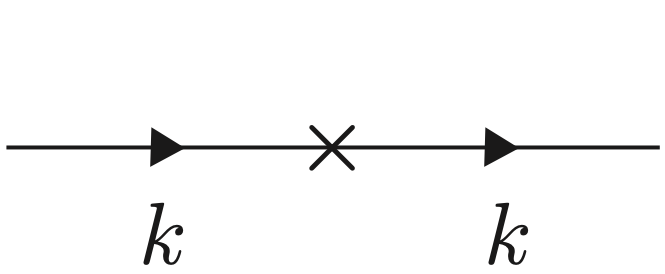
\includegraphics[align=c, width=0.2\linewidth]{pics/KG-ct.png}.
\end{aligned}
\end{equation}



\subsection{Self Energy Correction}
To second order, we consider the one-loop correction to the propagator: 
\begin{equation}\label{eq:rkg-self-energy}
\begin{aligned}
	i\tilde{\Delta}^{(2)}(k) 
	&= 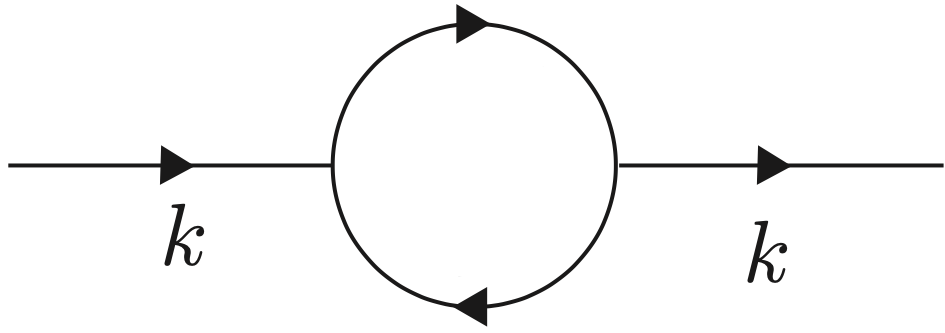
\includegraphics[align=c, width=0.2\linewidth]{pics/KG-1.png} \\
	&= i\tilde\Delta_0(k)\left[i\Sigma^{(2)}(k^2)\right]i\tilde\Delta_0(k),
\end{aligned}
\end{equation}
where the self energy term to the second order $i\Pi^{(2)}(k)$ is defined as:
\begin{equation}
	i\Sigma^{(2)}(k^2) 
	\equiv \frac{g^2}{2} \int \frac{d^dq}{(2\pi)^d} \tilde{\Delta}_0(q)\tilde{\Delta}_0(k-q) + (Ak^2-Bm^2).
\end{equation}

The coefficient $g^2/2$ comes from the symmetry factor in the diagram. We can also check the coefficient explicitly, by considering the expansion to the second order (we denote $\delta/\delta J(x_i)$ as $\delta_i$):
\begin{equation*}
\begin{aligned}
	\delta_{1}\delta_{2}\frac{1}{2!4!}\left[\frac{ig}{3!}\int d^dy \left(\frac{\delta}{\delta J(y)}\right)^3 \right]^2
	\left[-\frac{i}{2}\int d^dy_1 d^dy_2 J(y_1)\Delta(y_1-y_2)J(y_2)\right]^4.
\end{aligned}
\end{equation*}
The expansion gives the coefficient
\begin{equation*}
	\left(\frac{ig}{6}\right)^2\times \frac{1}{2!\times 4! \times 2^4}.
\end{equation*}
Now consider the combinatorial factor, which comes from the exchange of $\phi(x_i)$ in the propagator, the exchange of $\phi(x_i)$ in the vertex, the exchange of propagator in the diagram, and the change of vertices in the diagram:
\begin{equation*}
	(2!)^4\times(3!)^2\times(4\times 3)\times2.
\end{equation*}
Those two factors produce a $-g^2/2$ coefficient.
Note that in the self energy expressio, we put a $i$ factor in front of each propagator, which absorbs the minus sign.


Once we obtain the self energy, the one-loop corrected propagator has the form:
\begin{equation}
\begin{aligned}
	i\tilde{\Delta}(k) 
	&= i\tilde{\Delta}_0(k) + i\tilde{\Delta}_0(k)\left[\sum_{n=1}^{\infty}i\Sigma(k^2)\right]i\tilde{\Delta}_0(k) \\
	&= \frac{i}{\tilde{\Delta}^{-1}_0(k) - \Sigma(k^2)} \\
	&= \frac{i}{k^2-m^2-\Sigma(k^2)}.
\end{aligned}
\end{equation}
Now we are going to evaluate the divergent integral in the self energy expression, using the Feynman parameters:
\begin{equation*}
\begin{aligned}
&\int \frac{d^d q}{(2 \pi)^d} \frac{1}{q^{2}-m^2} \frac{1}{(k-q)^{2}-m^2} \\
=&\int \frac{d^d q}{(2 \pi)^d} \int_{0}^{1} d x \frac{1}{\left[q^{2}-m^2+x\left((q-k)^{2}-q^{2}\right)\right]^{2}} \\
=&\int_{0}^{1} d x \int \frac{d^d q}{(2 \pi)^d} \frac{1}{\left[(q-kx)^{2}-D\right]^{2}},
\end{aligned}
\end{equation*}
where $D=m^2-k^{2} x(1-x)$. Then we can shift $q \rightarrow q+kx$ leaving an integral that only depends on $q^{2}$. In this way,
\begin{equation*}
\Sigma(k^2) = \int_0^1 I(x)dx.
\end{equation*}
To evaluate the self-energy, it suffices to obtain the integral
\begin{equation*}
I(x) = \frac{g^2}{2i}\int \frac{d^d q}{(2 \pi)^d} \frac{1}{\left[q^{2}-D\right]^{2}}.
\end{equation*}

\begin{framedrmk}[Feyman Parameters]
We use Feynman's formula to combine denominators,
\begin{equation}
\frac{1}{A_{1} \ldots A_{n}}=\int d F_{n}\left(x_{1} A_{1}+\ldots+x_{n} A_{n}\right)^{-n},
\end{equation}
where the integration measure over the Feynman parameters $x_{i}$ is
\begin{equation}
\int d F_{n}=(n-1) ! \int_{0}^{1} d x_{1} \ldots d x_{n} \delta\left(x_{1}+\ldots+x_{n}-1\right).
\end{equation}
This measure is normalized so that $\int d F_{n} =1$. 
The simplest case is
\begin{equation}
\frac{1}{A B}=\int_{0}^{1} \frac{dx}{[A+(B-A) x]^{2}}
=\int_{0}^{1} \frac{\delta(x+y-1)}{[x A+y B]^{2}} dx dy.
\end{equation}
Other useful identities are
\begin{equation}
\begin{aligned}
\frac{1}{A B^{n}} &=\int_{0}^{1} dxdy\frac{\delta(x+y-1)n y^{n-1}}{[x A+y B]^{n+1}} , \\
\frac{1}{A B C} &=\int_{0}^{1} dxdydz \frac{2\delta(x+y+z-1)}{[x A+y B+z C]^{3}} .
\end{aligned}
\end{equation}
\end{framedrmk}


By making the Wick rotation $q^0 \rightarrow i q_E^0$, the integral becomes:\footnote{
	The $d$-dimensional solid angle is
	\begin{equation}
		\Omega_d = \frac{2\pi^{d/2}}{\Gamma(\frac{d}{2})},
	\end{equation}
	where $\Gamma(x)$ is the gamma function, satisfing
	\begin{equation}
		\Gamma(1+x) = x\Gamma(x),\ 
		\Gamma(\epsilon) = \frac{1}{\epsilon}-\gamma_E + O(\epsilon).
	\end{equation}
	In particular, $\Gamma(n+1)=n!$.
}
\begin{equation*}
I(x) = \frac{g}{2}\int \frac{d^d q_E}{(2 \pi)^d} \frac{1}{\left(q_E^{2}+D\right)^{2}}
=\frac{g\Omega_d}{2(2\pi)^d} \int dq \frac{q^{d-1}}{\left(q^{2}+D\right)^{2}}.
\end{equation*}


\subsubsection*{Dimensional Regularization}
We set the dimension to $d=6-\epsilon$, and rewrite the Lagrangian as
\begin{equation}
	\mathcal L 
	= Z_{\phi}\frac{1}{2} \partial^\mu\phi\partial_\mu\phi - 
	Z_m \frac{m^2}{2}\phi^2 + Z_g\frac{g\tilde{\mu}^{\epsilon/2}}{3!}\phi^3.
\end{equation}
Note that the coupling constant should be changed to $g\rightarrow g\tilde\mu^{\epsilon/2}$ where $\mu$ is of mass dimension $[1]$ in order to get the correct dimensionality. 
We then expand the expression to zeroth order of $\epsilon$.
A useful identity is:
\begin{equation}
\int d k \frac{k^{a}}{\left(k^{2}+D\right)^{b}}
= D^{\frac{a+1}{2}-b} 
\frac{\Gamma\left(\frac{a+1}{2}\right)\Gamma\left(b-\frac{a+1}{2}\right)}{2\Gamma(b)}.
\end{equation}
Actually, we can compute the integral and series expansion in \texttt{Mathematica} all together:
\FrameTBStyle{mathematica}
\begin{lstlisting}[style=mathematicaFrameTB]
omg=(2*Pi^(d/2))/(Gamma[d/2]);
cof=g^2*\[Mu]^(6-d)/2*omg/(2*Pi)^d;
int=cof*Integrate[q^(d-1)/(q^2+D)^2,{q,0,Infinity}][[1]];
map={g^2->\[Alpha]*(4*Pi)^3,EulerGamma->Subscript[\[Gamma],E]};
ans=Series[int/.{d->6-\[Epsilon]},{\[Epsilon],0,0}];
ans/.map//Simplify
\end{lstlisting}
The result is (where $\alpha\equiv g^2/(4\pi)^3$)
\begin{equation*}
I(x)= \frac{\alpha D}{2} \left[
\ln \left(\frac{De^{\gamma_E}}{4\pi\tilde\mu^2}\right)-\left(\frac{2}{\epsilon}+1\right)
\right]+O(\epsilon).
\end{equation*}
Now insert $D=m^2-k^{2} x(1-x)$. Note that
\begin{equation*}
\int_0^1 dx D = m^2-\frac{k^2}{6}.
\end{equation*}
This simplifies the result to
\begin{equation}
	\Sigma^{(2)}(k^2) = \frac{\alpha}{2}\left(\frac{2}{\epsilon}+1\right)\left(\frac{k^2}{2}-m^2\right)
	+ \frac{\alpha}{2}\int_0^1 dx D(x)\ln\left(\frac{D(x)}{\mu^2}\right),
\end{equation}
where we have replace $\tilde\mu$ with
\begin{equation}
\mu \equiv \sqrt{\frac{4\pi}{e^{\gamma_E}}}\tilde\mu.
\end{equation}



\subsubsection*{Renormalization}
 
The counter terms also contribute to the perturbative correction,
\begin{equation*}
\begin{aligned}
	\Sigma^{(2)}\left(k^{2}\right) 
	=& \frac{\alpha}{2} \int_{0}^{1} dx D \ln\left(\frac{D}{m^{2}}\right) 
	+\left\{\frac{\alpha}{6}\left[\frac{1}{\varepsilon}+\ln\left(\frac{\mu}{m}\right)+\frac{1}{2}\right]+A\right\} k^{2} \\
	&-\left\{\alpha\left[\frac{1}{\varepsilon}+\ln\left(\frac{\mu}{m}\right)+\frac{1}{2}\right]+B\right\} m^{2}+O\left(\alpha^{2}\right) .
\end{aligned}
\end{equation*}
Consider the on-shell condition for the subtraction:
\begin{equation}
	\Sigma(m^2) = \Sigma'(m^2)=0.
\end{equation}
Set $D_0 \equiv D(x)|_{k^2=m^2}=m^2(1-x+x^2)$, the self energy has the form:
\begin{equation}
	\Sigma^{(2)}(k^2)=\frac{\alpha}{2} \int_0^1dx D(x)\ln\left(\frac{D(x)}{D_0(x)}\right) + C_k k^2+C_m m^2.
\end{equation}
The condition $\Pi(m^2) =0$ requires
\begin{equation*}
	\Sigma^{(2)}(k^2)=\frac{\alpha}{2} \int_0^1dx D(x)\ln\left(\frac{D(x)}{D_0(x)}\right) + C_k (k^2-m^2).
\end{equation*}
The condition $\Pi'(m^2)=0$ requires
\begin{equation*}
\begin{aligned}
	\left.\frac{d\Sigma^{(2)}(k^2)}{dk^2}\right|_{k^2=m^2}
	&=\frac{\alpha}{2} \int_0^1dx \left.\left[
	\frac{D(x)}{dk^2}\ln\left(\frac{D(x)}{D_0(x)}\right)+D_0(x)
	\right]\right|_{q^2=m^2} + C_k  \\
	&= \frac{\alpha}{2}\int_0^1dx (x^2-x) + C_k \\
	&= C_k-\frac{\alpha}{12} = 0.
\end{aligned}
\end{equation*}
In this way, we obtained the renormalized self-energy:
\begin{equation}
	\Sigma^{(2)}(k^2)=\frac{\alpha}{2} \int_0^1dx D(x)\ln\left(\frac{D(x)}{D_0(x)}\right) + \frac{\alpha}{12}(k^2-m^2).
\end{equation}

On the other hand, we chan choose the $\overline{\mathrm{MS}}$ subtraction scheme, i.e.,
\begin{equation}
	A = -\frac{\alpha}{6\epsilon},\ 
	B = -\frac{\alpha}{\epsilon}.
\end{equation}
The self energy under $\overline{\mathrm{MS}}$ scheme will depend on the the mass scale $\mu$ we choose:
\begin{equation}
	\Sigma^{(2)}\left(k^{2}\right) 
	= \frac{\alpha}{2} \int_{0}^{1} dx D \ln\left(\frac{D}{m^{2}}\right) 
	+\alpha\left[\ln\left(\frac{\mu}{m}\right)+\frac{1}{2}\right]\left(\frac{k^2}{6}-m^2\right).
\end{equation}


\subsection{Vertex Correction}
Now consider the simplest one-loop correction to the vertex function (together with the counter term):
\begin{equation}
\begin{aligned}
	i V_3^{(3)}(k_{1}, k_{2}, k_{3})
	&= 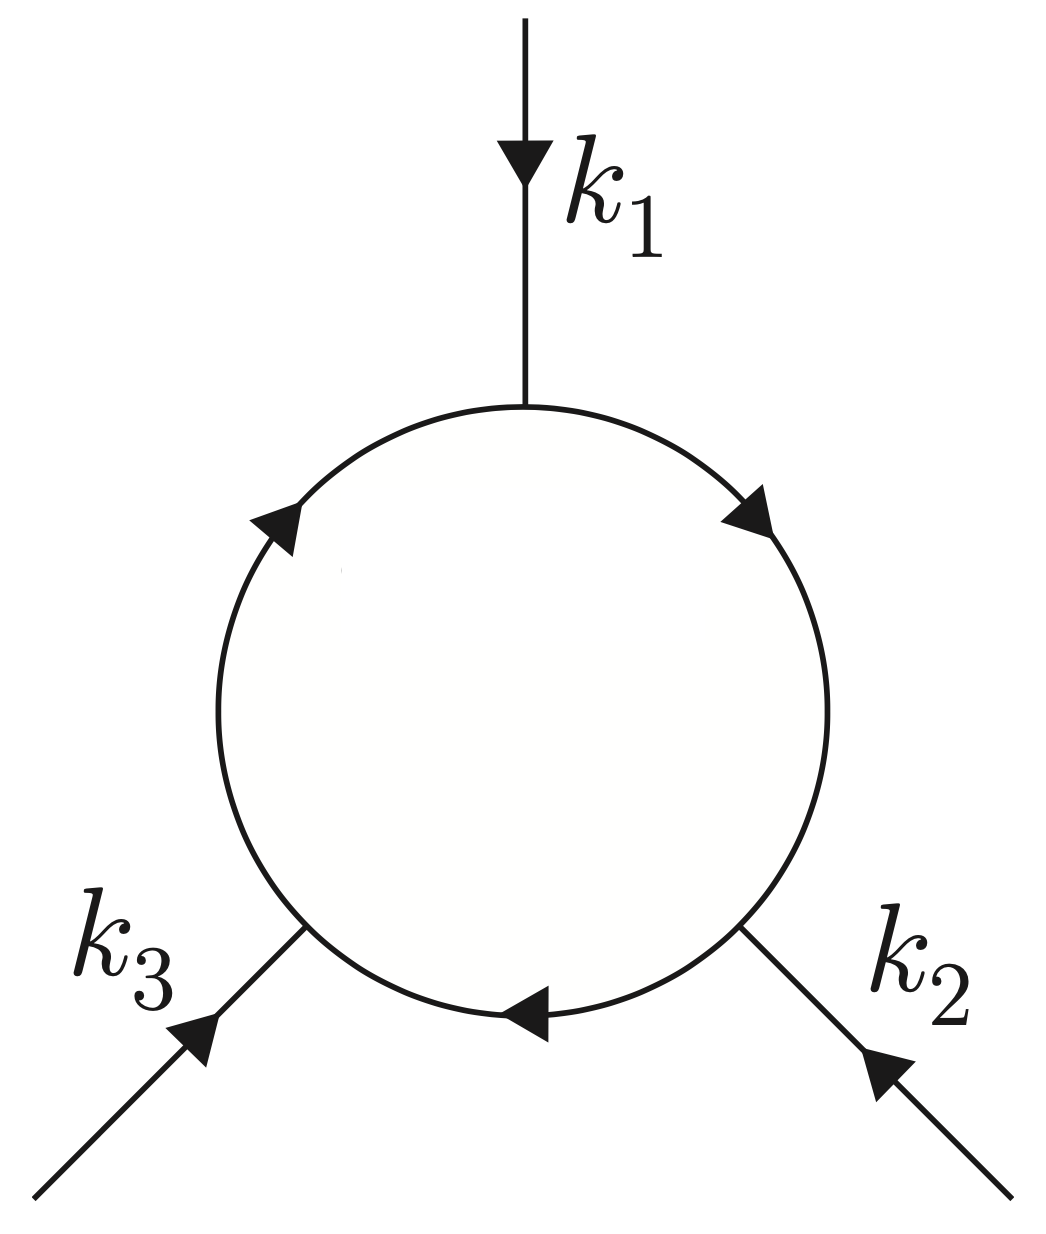
\includegraphics[align=c, width=0.4\linewidth]{pics/KG-2.png} \\
	&= (ig)^3i^3 \int \frac{d^{a} q}{(2 \pi)^{d}} \tilde{\Delta}(q-k_{1}) \tilde{\Delta}(q+k_{2}) \tilde{\Delta}(q) + i Cg,
\end{aligned}
\end{equation}
Using the Feynman parameter, the integrant is
\begin{equation*}
\tilde{\Delta}(q-k_{1}) \tilde{\Delta}(q+k_{2}) \tilde{\Delta}(q) 
= \int d F_3\frac{1}{(q^2-D)^3}
\end{equation*}
where we have shift the value of $q$, and $D$ can be evaluate by the following code:
\begin{lstlisting}[style=mathematicaFrameTB]
A1=(l-k1)^2-m^2;
A2=(l+k2)^2-m^2;
A3=(l)^2-m^2;
{c,b,a}=CoefficientList[x1*A1+x2*A2+(1-x1-x2)*A3,{l}];
-c+b^2/(4*a)//Expand
\end{lstlisting}
The result is
\begin{equation*}
D = m^2-k_1^2 x_1 (1- x_1)-k_2^2 x_2 (1- x_2)-2 k_1 k_2 x_1 x_2.
\end{equation*}
The same procedure gives:
\begin{equation}
	V_3^{(3)}/g = \int dF_3 I(x_1,x_2,x_3) + C,
\end{equation}
where
\begin{equation*}
I(x_1,x_2,x_3) = \frac{g^2 \Omega_d}{(2\pi)^d} \int dq \frac{q^{d-1}}{(q^2+D)^3}.
\end{equation*}
The same regularization procedure in \texttt{Mathematica}:
\begin{lstlisting}[style=mathematicaFrameTB]
omg=(2*Pi^(d/2))/(Gamma[d/2]);
cof=g^2*\[Mu]^(6-d)*omg/(2*Pi)^d;
int=cof*Integrate[q^(d-1)/(q^2+D)^3,{q,0,Infinity}][[1]];
map={g^2->\[Alpha]*(4*Pi)^3,EulerGamma->Subscript[\[Gamma],E]};
ans=Series[int/.{d->6-\[Epsilon]},{\[Epsilon], 0, 0}];
ans/.map//Simplify
\end{lstlisting}
The result is
\begin{equation}
\begin{aligned}
	V_3^{(3)}/g 
	&= \frac{\alpha}{\epsilon}
	+ \frac{\alpha}{2}\int dF_3 \ln\left(\frac{4\pi\tilde{\mu}^2e^{-\gamma_E}}{D}\right) 
	+ C + O(\epsilon) \\
	&= \frac{\alpha}{\epsilon}
	+ \alpha\ln\left(\frac{\mu}{m}\right)
	- \frac{\alpha}{2}\int dF_3 \ln\left(\frac{D}{m}\right)
	+C.
\end{aligned}
\end{equation}
The on-shell subtraction requires 
\begin{equation}
V_3(0,0,0) = g,
\end{equation}
which gives
\begin{equation}
	C = -\frac{\alpha}{\epsilon}-\alpha \ln\left(\frac{\mu}{m}\right).
\end{equation}
So the vertex function to the third order is
\begin{equation}
	V_3(k_1,k_2,k_3) = g\left\{1-\frac{\alpha}{2} \int dF_3 \ln\left[\frac{D(x_1,x_2,x_3)}{m}\right] \right\}.
\end{equation}
The $\overline{\mathrm{MS}}$ scheme, on the other hand, sets
\begin{equation}
	C = -\frac{\alpha}{\epsilon}.
\end{equation}



\subsection{Renormalization Group}
We fist summarize the normalization factor obtained on the one-loop level (with $\overline{\mathrm{MS}}$ subtraction scheme):
\begin{equation}
\begin{aligned}
	Z_{\phi} &= 1-\frac{\alpha}{6\epsilon} + O(\alpha^2), \\
	Z_{m} &= 1-\frac{\alpha}{\epsilon}+ O(\alpha^2), \\
	Z_{g} &= 1-\frac{\alpha}{\epsilon}+ O(\alpha^2).
\end{aligned}
\end{equation}
For the renormalized Lagrangian in ($6-\epsilon$)-dimension
\begin{equation}
	\mathcal L 
	= Z_{\phi}\frac{1}{2} \partial^\mu\phi\partial_\mu\phi - 
	Z_m \frac{m^2}{2}\phi^2 + Z_g\frac{g\tilde{\mu}^{\epsilon/2}}{3!}\phi^3,
\end{equation}
the factors relate the original field and bare coefficients
\begin{equation}
	\phi_0 = Z_\phi^{1/2}\phi,\ 
	m_0 = Z_m^{1/2} Z_\phi^{-1/2}m,\ 
	g_0 = Z_g Z_{\phi}^{-3/2} \tilde{\mu}^{\epsilon/2}g.
\end{equation}
The renormalization group requires that the bare parameter is independent of the mass scale $\mu$ we choose, that is:
\begin{equation}
	\frac{d\phi_0}{d \ln \mu} 
	= \frac{dm_0}{d \ln \mu}
	= \frac{dg_0}{d \ln \mu}
	= 0.
\end{equation}


\subsubsection*{Beta Function}
Star with $g_0$, it is more convenient to use 
\begin{equation}
\alpha_0 
\equiv \frac{g_0^2}{4\pi} 
= Z_g^2 Z_{\phi}^{-3}\tilde{\mu}^{\epsilon}\alpha.
\end{equation}
Take logarithm on both side:
\begin{equation}
\ln \alpha_0 = \ln(Z_g^2 Z_{\phi}^{-3}) 
+ \ln \alpha + \epsilon\ln{\tilde\mu}.
\end{equation}
The RG equation is
\begin{equation}
\frac{d \ln \alpha_0}{d \ln \mu} = 
\frac{d \ln(Z_g^2 Z_{\phi}^{-3}) }{d \alpha}\frac{d \alpha}{d\ln \mu} +
\frac{1}{\alpha}\frac{d \alpha}{d \ln \mu} + \epsilon
=0.
\end{equation}
To the first order of $\alpha$:
\begin{equation}
\begin{aligned}
	\frac{d \ln(Z_g^2 Z_{\phi}^{-3}) }{d \alpha}
	=\frac{d}{d\alpha}\left(-\frac{2\alpha}{\epsilon}+\frac{\alpha}{2\epsilon}\right) 
	= -\frac{3}{2\epsilon},
\end{aligned}
\end{equation}
which leads to
\begin{equation}
	\frac{d\alpha}{d\ln \mu}\left(1-\frac{3\alpha}{2\epsilon}+O(\alpha^2)\right)+\epsilon\alpha = 0.
\end{equation}
The beta function is defined as
\begin{equation}
	\beta(\alpha) = \frac{d\alpha}{d\ln \mu} = \beta_1 \alpha + \beta_2 \alpha^2 + O(\alpha^3).
\end{equation}
Insert such definition into the original expression, and keep track of the order of $\alpha$, we get
\begin{equation}
	(\beta_1+\epsilon)\alpha + \left(\beta_2-\frac{3\beta_1}{2\epsilon}\right)\alpha^2 + O(\alpha^3) = 0.
\end{equation}
The beta function is
\begin{equation}
	\beta(\alpha) = -\epsilon \alpha -\frac{3}{2}\alpha^2 + O(\alpha^3).
\end{equation}



\subsubsection*{Anomalous Dimension}
Consider the RG equation with bare mass:
\begin{equation}
\begin{aligned}
\frac{d\ln m_0}{d\ln \mu} 
&= \frac{1}{2}\frac{d(\ln Z_m - \ln Z_\phi)}{d\alpha}\frac{d\alpha}{d\ln\mu}
	+\frac{1}{m}\frac{d m}{d\ln \mu} \\
&= \frac{5\alpha}{12}+\frac{1}{m}\frac{d m}{d\ln \mu} + O(\alpha^2) = 0.
\end{aligned}
\end{equation}
We get the anomalous dimension of the mass:
\begin{equation}
\gamma_m(\alpha) \equiv \frac{1}{m}\frac{d m}{d\ln \mu} 
= -\frac{5\alpha}{12}+O(\alpha^2).
\end{equation}
Also, for the bare field
\begin{equation}
\frac{d\ln\phi_0}{d\ln\mu} = \frac{1}{2} \frac{d\ln Z_{\phi}}{d\ln\mu} 
+ \frac{d\ln\phi}{d\ln\mu} = 0.
\end{equation}
We can define the anomalous dimension of the field as
\begin{equation}
\gamma_{\phi} \equiv \frac{1}{2}\frac{d \ln Z_\phi}{d\ln\mu}
= \frac{1}{2}\frac{d \ln Z_\phi}{d\alpha}\frac{d\alpha}{d\ln\mu}
= \frac{\alpha}{12} +O(\alpha^2).
\end{equation}



\subsubsection*{Callan-Symanzik Equation}
Consider the bare propagator:
\begin{equation}
\tilde{\Delta}_0(k) = Z_\phi \tilde{\Delta}(k)
\end{equation}
The RG condition for the bare propagator gives:
\begin{equation*}
\frac{d\ln\tilde{\Delta}_0(k)}{d \ln\mu}
=\frac{d\ln Z_\phi}{d\ln\mu}+\frac{1}{\tilde{\Delta}(k)}\left(
	\frac{\partial}{\partial\ln\mu} +
	\frac{d\alpha}{d\ln\mu}\frac{\partial}{\partial\alpha} +
	\frac{dm}{d\ln\mu}\frac{\partial}{\partial m}
\right)\tilde{\Delta}(k)=0.
\end{equation*}
The Callan-Symanzik equation is
\begin{equation}
	\left(
	2\gamma_\phi+
	\frac{\partial}{\partial\ln\mu} +
	\beta(\alpha)\frac{\partial}{\partial\alpha} +
	\gamma_m(\alpha)m\frac{\partial}{\partial m}
\right)\tilde{\Delta}(k)=0.
\end{equation}

\section{Real $\phi^4$ Theory}
In this section, we consider the real Klein-Gordon field with $\phi^4$ interaction.
The field $\phi$ has mass dimension $[\frac{d-2}{2}]=[1]$, so the critical dimension is $d=4$, where the coupling constant $g$ is dimensionless.
For dimensional regulation purpose, we write the renormalized Lagrangian on $(4-\epsilon)$-dimensional space-time as
\begin{equation}
	\mathcal{L}
	= Z_{\phi}\frac{1}{2} \partial^\mu\phi\partial_\mu\phi - 
	Z_m \frac{m^2}{2}\phi^2 - Z_g\frac{g \tilde{\mu}^\epsilon}{4!}\phi^4,
\end{equation}
where we have introduced a mass scale $\tilde \mu$.
As the $\phi^3$ theory, we can rewrite the Lagrangian as:
\begin{equation}
	\mathcal L = \mathcal L_0 + \mathcal L_{\mathrm{int}} + \mathcal L_{\mathrm{ct}}.
\end{equation}
In the following we investigate the loop correction to the mass and the coupling constant.


\subsection{One-loop Correction}
\subsubsection*{Self-energy}
Following the same procedure, the one-loop self-energy correction is (with counter terms):
\begin{equation}
\begin{aligned}
	i\Sigma(k^2) 
	&= 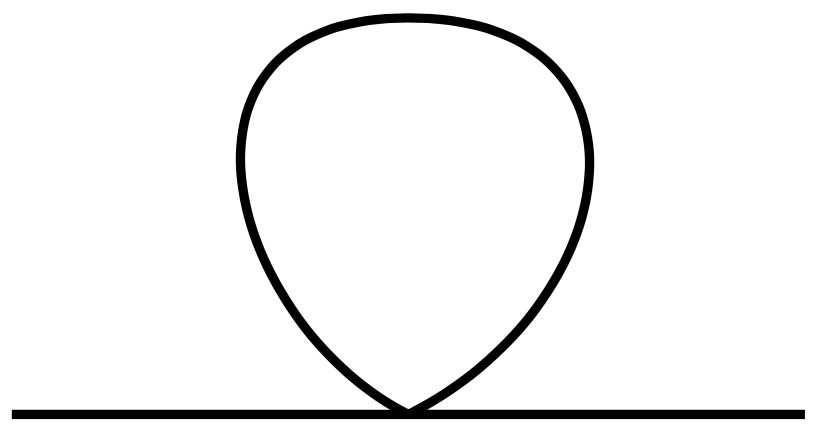
\includegraphics[align=c, width=0.4\linewidth]{pics/KG-3.png} \\
	&= -\frac{g\tilde{\mu}^\epsilon}{2}\int \frac{d^d q}{(2\pi)^d} \frac{1}{q^2-m^2} + i(Ak^2-Bm^2).
\end{aligned}
\end{equation}
After the Wick rotation, 
\begin{equation}
	\Sigma(k^2) = -\frac{g\tilde{\mu}^\epsilon}{2}\frac{\Omega_d}{(2\pi)^d} \int \frac{q^{d-1} dq}{q^2+m^2} + (Ak^2-Bm^2).
\end{equation}
The dimensional regulation is carried out using the following code:
\begin{lstlisting}[style=mathematicaFrameTB]
omg=(2*Pi^(d/2))/(Gamma[d/2]);
cof=g*\[Mu]^(4-d)/2*omg/(2*Pi)^d;
int=cof*Integrate[q^(d-1)/(q^2+m^2),{q,0,Infinity}][[1]];
map={EulerGamma->Subscript[\[Gamma],E]};
ans=Series[int/.{d->4-\[Epsilon]},{\[Epsilon],0,0}];
ans/.map//Simplify
\end{lstlisting}
The result is
\begin{equation}
	\Sigma(k^2) = \frac{g m^2}{32\pi^2} \left[\frac{2}{\epsilon}+1+\log \left(\frac{4 \pi \tilde{\mu}^2 e^{-\gamma_E}}{m^2}\right)\right]+(Ak^2-Bm^2)+O(\epsilon).
\end{equation}
Using the $\overline{\mathrm{MS}}$ renormalization scheme, we set
\begin{equation}
	A = 0,\ B = \frac{g}{16\pi^2\epsilon}.
\end{equation}
The result is
\begin{equation}
	\Sigma(k^2) = \frac{g m^2}{16\pi^2} \log \left(\frac{\mu}{m}\right)
	+\frac{g m^2}{32\pi^2}+O(\epsilon).
\end{equation}

\subsubsection*{Vertex Correction}
Now consider the vertex correction.
The vertex correction to the lowest order (with the counter term) is
\begin{equation}
\begin{aligned}
	iV_4^{(2)}(k_1,k_2,k_3,k_4) 
	&= 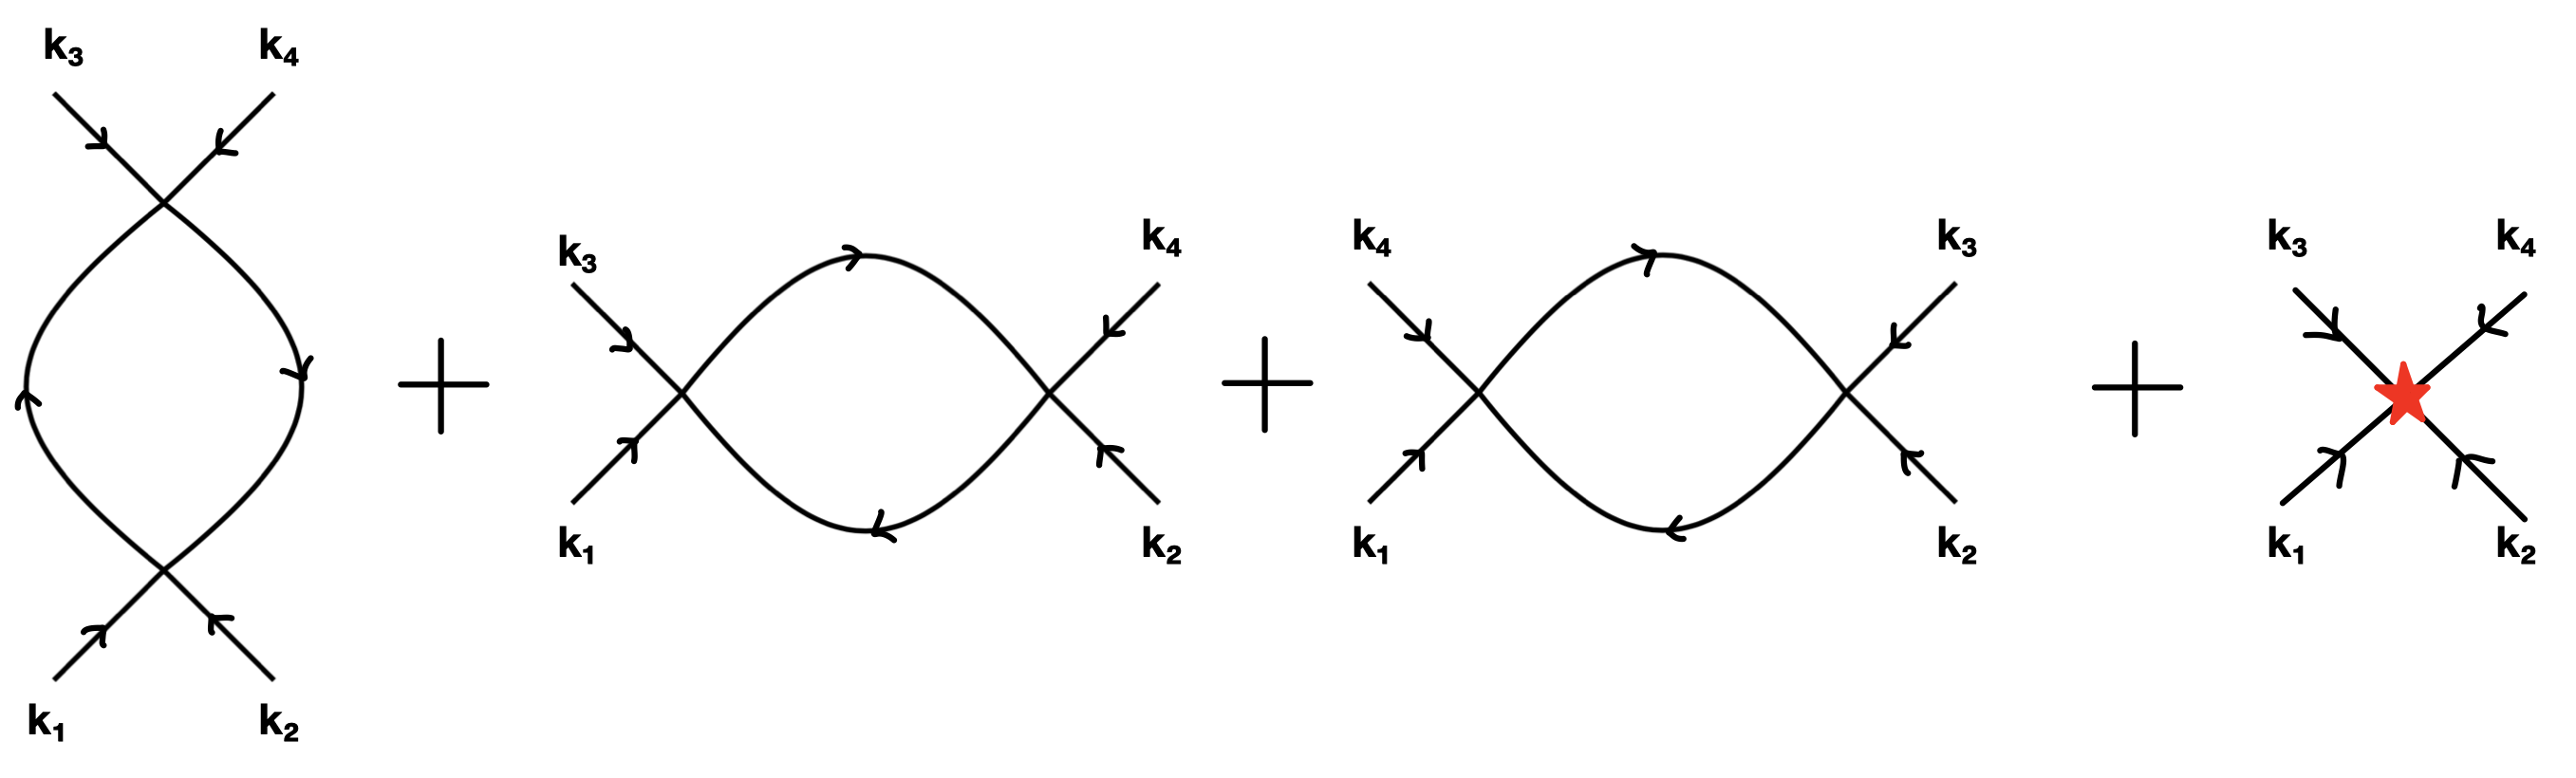
\includegraphics[align=c, width=0.6\linewidth]{pics/KG-4.png}\\
	&= \frac{g^2}{2} \left[iF(s)+iF(t)+iF(u)\right] -iCg,
\end{aligned}
\end{equation}
where
\begin{equation}
	s = (k_1+k_2)^2,\ 
	t = (k_1+k_3)^2,\ 
	u = (k_1+k_4)^2,
\end{equation}
and
\begin{eqnarray}
	iF(k^2) 
	&=& \tilde{\mu}^{\epsilon}\int \frac{d^d q}{(2\pi)^d} \tilde{\Delta}_0(q)\tilde{\Delta}_0(q+k) \\
	&=& \frac{i\tilde{\mu}^{\epsilon}\Omega_d}{(2\pi)^d} \int_0^1 dx \int \frac{q^{d-1}dq}{\left[q^2+m^2+x(1-x)k^2\right]^2}.
\end{eqnarray}
Then we carry out the calculation (set $D(k^2,x)=m^2+x(1-x)k^2$)
\begin{lstlisting}[style=mathematicaFrameTB]
omg=(2*Pi^(d/2))/(Gamma[d/2]);
cof=g^2*\[Mu]^(4-d)/2*omg/(2*Pi)^d;
int=cof*Integrate[q^(d-1)/(q^2+D)^2,{q,0,Infinity}][[1]];
map={EulerGamma->Subscript[\[Gamma],E]};
ans=Series[int/.{d->4-\[Epsilon]},{\[Epsilon],0,0}];
ans/.map//Simplify
\end{lstlisting}
The result is:
\begin{equation}
\begin{aligned}
	F(s) &= \frac{1}{8\pi^2\epsilon} + \frac{1}{16\pi^2}\int_0^1 dx \ln \left(\frac{4\pi \tilde{\mu}^2 e^{-\gamma_E}}{D}\right) \\
	&= \frac{1}{8\pi^2\epsilon} +\frac{1}{8\pi^2}\ln \left(\frac{\mu}{m}\right) - \frac{1}{16\pi^2}\int_0^1 dx \ln\left(\frac{D(s,x)}{m^2}\right).
\end{aligned}
\end{equation}
The $\overline{\mathrm{MS}}$ scheme absorbs the $\frac{1}{8\pi^2\epsilon}$ term, i.e.,
\begin{equation}
	C = \frac{3g}{16\pi^2}.
\end{equation}
The result is:
\begin{equation}
	V_4(k_1,k_2,k_3,k_4) = -g+\frac{g^2}{32\pi^2}\int_0^1 dx \ln\left(\frac{\mu^6}{D(s,x)D(t,x)D(u,x)}\right).
\end{equation}
To summarize, the normalization is:
\begin{eqnarray}
	Z_{\phi} &=& 1, \\
	Z_{m} &=& 1+\frac{g}{16\pi^2 \epsilon}, \\
	Z_{g} &=& 1+\frac{3g}{16\pi^2 \epsilon}.
\end{eqnarray}


\subsection{Renormalization Group}
Now consider the RG equation for the one-loop correction. 
The bare parameters are:
\begin{equation}
	g_0 = Z_g g\tilde{\mu}^{\epsilon},\ 
	m_0 = Z_m^{1/2} m,
\end{equation}
The RG conditions are:
\begin{eqnarray}
	\frac{d g_0}{d\ln \mu}
	&=& \left(\frac{3}{16\pi^2 \epsilon} + \frac{1}{g}\right)\frac{dg}{d\ln \mu} + \epsilon = 0, \\
	\frac{d m_0}{d\ln \mu}
	&=& \frac{1}{32\pi^2 \epsilon}\frac{dg}{d\ln \mu} + \frac{1}{m}\frac{dm}{d \ln \mu} = 0.
\end{eqnarray}
Consider the series expansion of beta function:
\begin{equation}
	\beta(g) = \frac{dg}{d\ln \mu} = \beta_1 g + \beta_2 g^2 +O(g^3).
\end{equation}
The beta function is
\begin{equation}
	\beta(g) = -\epsilon g + \frac{3g^2}{16\pi^2} + O(g^3).
\end{equation}
The anomalous dimension of mass is
\begin{equation}
	\gamma_m = \frac{1}{m}\frac{dm}{d \ln \mu} = \frac{g}{32\pi^2}+O(g^2)
\end{equation}




\chapter{Quantum Electrodynamics}

The Lagrangian for quantum electrodynamics is
\begin{equation}
\begin{aligned}
	\mathcal{L}_{\mathrm{QED}}
	&= \bar\psi \left(i\gamma^\mu \partial_\mu - m\right)\psi - \frac{1}{4}F_{\mu\nu}F^{\mu\nu} -eA_\mu \bar\psi\gamma^\mu  \psi \\
	&= \mathcal{L}_{\mathrm{Dirac}}+\mathcal{L}_{\mathrm{Maxwell}}+\mathcal{L}_{\mathrm{int}},
\end{aligned}
\end{equation}
where
\begin{equation}
	F_{\mu\nu} = \partial_\mu A_\nu - \partial_\nu A_\nu = (dA)_{\mu\nu}.
\end{equation}
The Lagrangian is invariant under the gauge transformation:
\begin{equation}
\begin{aligned}
	\psi(x) &\rightarrow e^{-ie\alpha(x)}\psi(x), \\
	A^\mu(x) &\rightarrow A^\mu(x) + \partial^\mu \alpha(x).
\end{aligned}
\end{equation}
It is convenient to rewrite Lagrangian as
\begin{equation}
	\mathcal{L}_{\mathrm{QED}}
	= \bar\psi \left(i\cancel{D} - m\right)\psi - \frac{1}{4}F_{\mu\nu}F^{\mu\nu},
\end{equation}
where we have define the covariant derivative as:
\begin{equation}
	\cancel{D} = \gamma^\mu D_\mu 
	= \gamma^\mu [\partial_\mu + i e A_\mu(x)]
	= \cancel{\partial} + ie \cancel{A}.
\end{equation}


\section{Free Field Theory}

\subsection{Dirac Field}
The free Dirac field is
\begin{equation}
	\mathcal{L}_{\mathrm{Dirac}}
	= \bar\psi \left(i\gamma^\mu \partial_\mu - m\right)\psi
\end{equation}
Consider the partition function with source
\begin{equation}
\begin{aligned}
	Z_{\mathrm{Dirac}}[J]
	&= \int D[\bar\psi,\psi] \exp\left[i\int d^dx \left(\mathcal{L}_{\mathrm{Dirac}}+\bar{\eta}\psi + \bar\psi\eta \right) \right] \\
	&= Z_{\mathrm{Dirac}}[0] \exp\left[-i\int d^dx_1 d^d x_2 \bar{\eta}(x_1)\cdot D_F(x_1-x_2)\cdot \eta(x_2) \right].
\end{aligned}
\end{equation}
where
\begin{equation}
	D_F(x_1-x_2) = \int \frac{d^d k}{(2\pi)^d} \frac{e^{-i k \cdot (x_1-x_2)}}{\cancel{k}-m}
	= \int \frac{d^d k}{(2\pi)^d} e^{-i k \cdot (x_1-x_2)} \frac{\cancel{k}+m}{k^2-m^2}.
\end{equation}
Note that the propagator is\footnote{The sign in the variational derivative comes from the anti-commutation relation of the fermionic fields.}
\begin{equation}
\begin{aligned}
	\langle 0| T \psi(x_1) \bar\psi(x_2) |0\rangle
	&= \frac{1}{Z_{\mathrm{Dirac}}[0]}\frac{\delta}{i\delta \bar{\eta}(x_1))}\frac{i\delta}{\delta(\eta(x_2))} Z_{\mathrm{Dirac}}[J] \\
	&= i D_F(x_1-x_2).
\end{aligned}
\end{equation}

\subsection{Electromagnetic Field}
The Lagrangian for the classical electromagnetic field is
\begin{equation}
	\mathcal{L} = -\frac{1}{4}F_{\mu\nu}F^{\mu\nu}+A_\mu J^\mu.
\end{equation}
Consider the partition function
\begin{equation}
	\frac{Z_{\mathrm{maxwell}}[J]}{Z_{\mathrm{maxwell}}[0]}
	= \exp\left[-\frac{i}{2}\int dx_1 dx_2 J_\mu(x_1) \Pi^{\mu\nu}(x_1-x_2) J_\nu(x_2) \right].
\end{equation}

The propagator is
\begin{equation}
	\Pi^{\mu\nu}(x_1-x_2) = \int \frac{d^d k}{(2\pi)^d} e^{-ik\cdot(x_1-x_2)}\frac{-g^{\mu\nu}+(1-\xi)k^\mu k^\nu}{k^2}.
\end{equation}


\subsection{Perturbation Theory}
As with the scalar field, 
\begin{equation}
	Z[\bar\eta,\eta,J] = \exp\left\{i\int d^dx \mathcal{L}_{\mathrm{int}}\left[\frac{\delta}{i\delta J},\frac{\delta}{i\delta \eta},\frac{i\delta}{\delta \bar\eta}\right]\right\} Z_0[\bar\eta,\eta,J].
\end{equation}
We use the dimensional regularization by default. 
Note that $\psi$ has the mass dimension $[\frac{d-1}{2}]$, $A^\mu$ had the mass dimension $[\frac{d}{2}-1]$, and $e$ has the mass dimension $[2-\frac{d}{2}]$.
When $d=4-\epsilon$, we replace $e$ with $e \tilde{\mu}^{\epsilon/2}$, so that to make the coupling constant $e$ dimensionless.

The renormalized Lagrangian is
\begin{equation}
\begin{aligned}
	\mathcal L 
		&= Z_{\psi} \bar\psi_R(i\gamma^\mu \partial_\mu)\psi_R 
		-Z_m m \bar\psi_R\psi_R 
		+ \frac{1}{4} Z_{A} F_{R,\mu\nu}F_R^{\mu\nu} - Z_e e_R A_R^\mu \bar\psi_R\gamma^\mu \psi_R \\
		&= \mathcal{L}_0 + \mathcal{L}_{\mathrm{int}} + \mathcal{L}_{\mathrm{ct}}.
\end{aligned}
\end{equation}
The we define the coefficients
\begin{equation}
	\delta_{\psi} = Z_\phi - 1,\ 
	\delta_{m} = Z_m - 1,\ 
	\delta_Z = Z_A - 1, \ 
	\delta_e = Z_e - 1.
\end{equation}
The counter term also contribute to the perturbative expansion like the interactions.


\begin{framedexpl}[One-loop Correction to Electron Propagator]
Consider the diagram
\begin{equation*}
	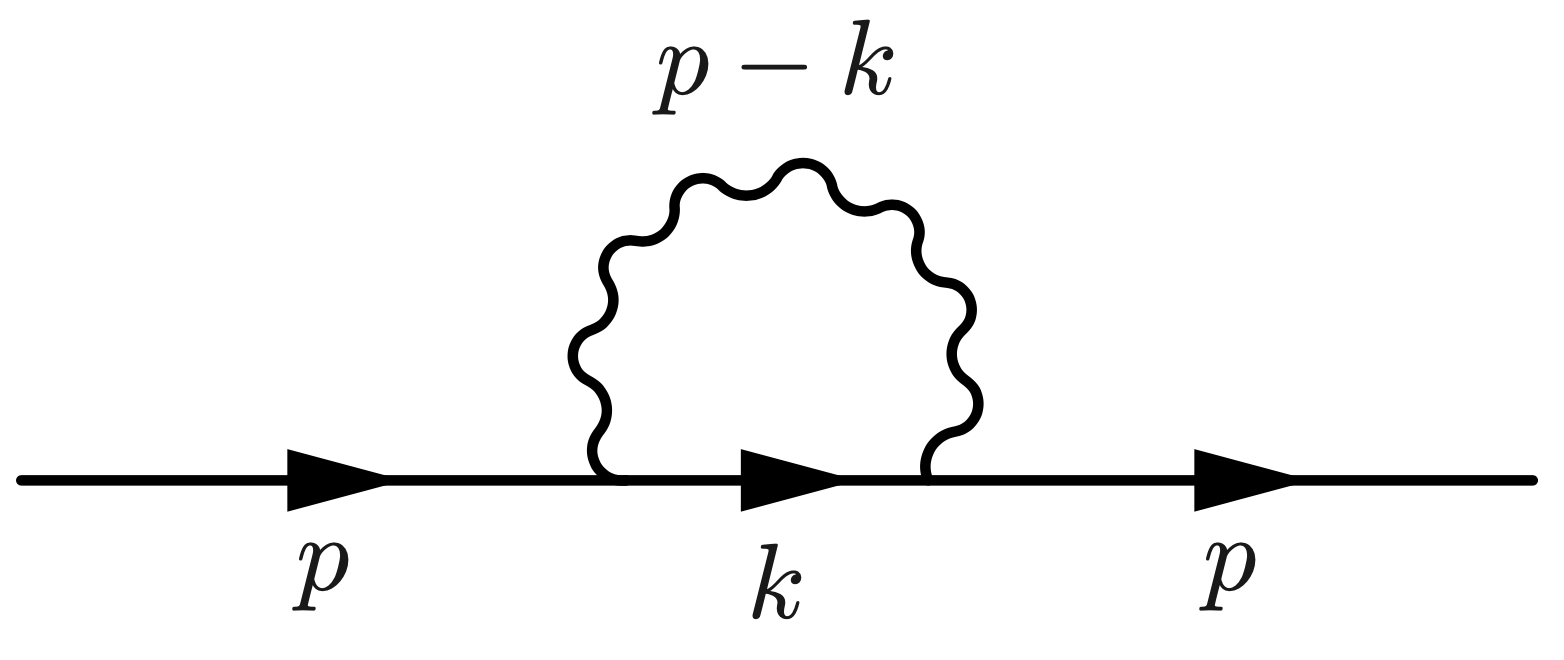
\includegraphics[width=0.3\linewidth]{pics/QED-1.png}
\end{equation*}
This contains 3 electron propagator, 1 photon propagator, and 2 vertices.
The coefficient is (omit all the integration and summation for simplicity):
\begin{equation*}
	iD_F^{(2)}(p) \sim \frac{\delta^2}{\delta\bar\eta \delta\eta}\frac{1}{2!}
	\left(\frac{-ie\gamma^\mu_{\alpha\beta}\delta^3}{i\delta J^\mu \delta\eta_{\alpha} \delta\bar\eta_{\beta}}\right)^2 
	\frac{1}{3!}\left(-i \bar\eta_{\alpha} D_F^{\alpha\beta} \eta_{\beta} \right)^3 
	\left(-\frac{i}{2} J^\mu\Pi_{\mu\nu}J^{\nu} \right).
\end{equation*}
First consider the scalar coefficient. 
Since there is no additional symmetry, the abstract value is $e^2$.
There is an additional sign factor by the proper order of the fermion operators:
\begin{equation*}
	\frac{\delta^2}{\delta\bar\eta_f \delta\eta_i} \frac{\delta^2}{\delta\eta_1 \delta\bar\eta_1} \frac{\delta^2}{\delta\eta_2 \delta\bar\eta_2}
	= - \frac{\delta}{\delta \eta_i}\frac{\delta^2}{\delta\bar\eta_1 \delta\eta_1}\frac{\delta^2}{\delta\bar\eta_2 \delta\eta_2}\frac{\delta}{\delta \bar\eta_f}.
\end{equation*}

Then consider the tensor contraction, 
\begin{equation*}
	\Pi_{\mu\nu} D_F^{\alpha\lambda}\gamma^\mu_{\lambda\rho} D_F^{\rho\tau} \gamma^\nu_{\tau\sigma} D_F^{\sigma\beta}.
\end{equation*}

The total amplitude is
\begin{equation*}
\begin{aligned}
	iD_F^{(2)}(p)
	&= -e^2\int\frac{d^4 k}{(2\pi)^4} \Pi_{\mu\nu}(p-k) \left[D_F(p) \gamma^\mu D_F(k) \gamma^\nu D_F(p)\right]_{\alpha\beta} \\
	&= iD_F(p) i\Sigma(p^2) iD_F(p),
\end{aligned}
\end{equation*}
where $i\Sigma(p^2)$ is the self energy:
\begin{equation}
	i\Sigma(p^2)
	= e^2\int\frac{d^4 k}{(2\pi)^4} \Pi_{\mu\nu}(p-k) \gamma^\mu D_F(k) \gamma^\nu ,
	\label{eq:QED-ele-loop-prop}
\end{equation}
\end{framedexpl}


\begin{framedexpl}[One-loop Correction to Photon Propagator]
Consider the diagram
\begin{equation*}
	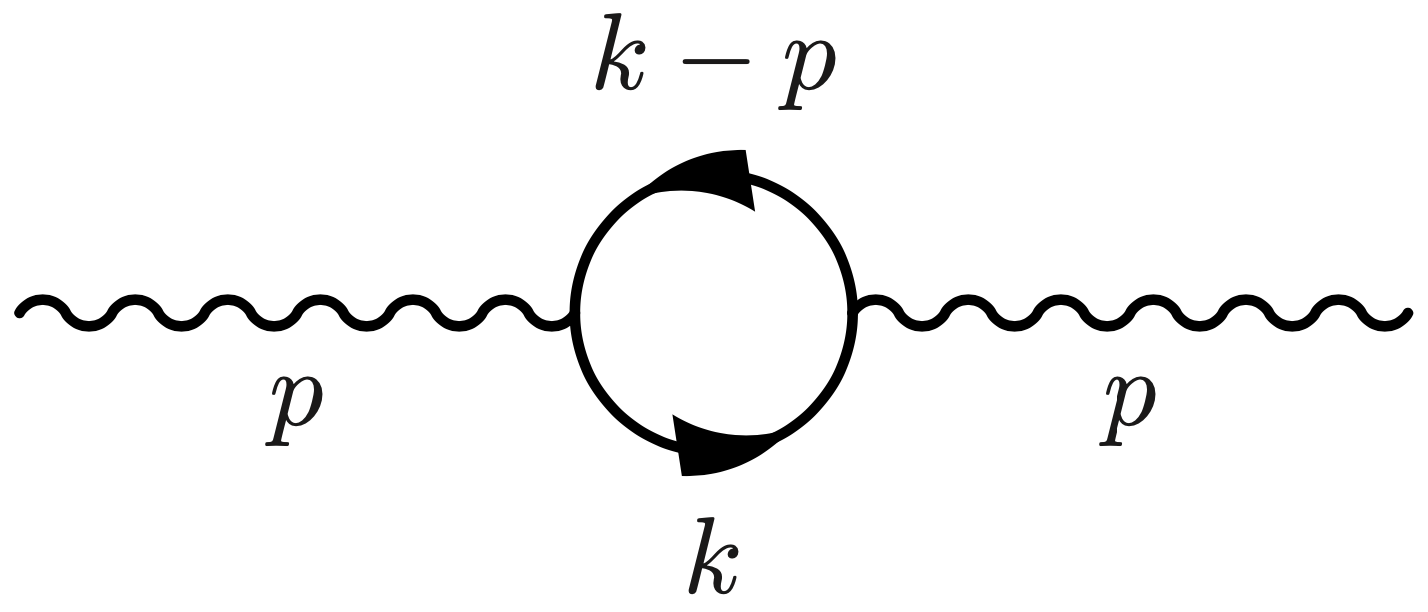
\includegraphics[width=0.3\linewidth]{pics/QED-2.png}
\end{equation*}
There is 2 electron propagator, 2 photon propagator, and 2 vertices.
Consider the perturbative expansion:
\begin{equation*}
	i\Pi^{(2)}(p) \sim \frac{\delta^2}{i\delta J i\delta J}\frac{1}{2!}
	\left(\frac{-e\gamma^\mu_{\alpha\beta}\delta^3}{\delta J^\mu \delta\eta_{\alpha} \delta\bar\eta_{\beta}}\right)^2 
	\frac{1}{2!}\left(-i \bar\eta_{\alpha} D_F^{\alpha\beta} \eta_{\beta} \right)^2 
	\frac{1}{2!}\left(\frac{i}{2} J^\mu \Pi_{\mu\nu} J^{\nu} \right)^2.
\end{equation*}
The diagram has no symmetry factor, but with a $-1$ sign, which is canceled out by the operator reordering:
\begin{equation}
	\bar\eta_\beta D_F^{\beta\tau} \eta_\tau \bar\eta_\sigma D_F^{\sigma\alpha} \eta_\alpha
	= -\eta_\alpha\bar\eta_\beta D_F^{\beta\tau} \eta_\tau \bar\eta_\sigma D_F^{\sigma\alpha}.
\end{equation}
The overall value is $e^2$.
 
Then consider the tensor contraction, 
\begin{equation*}
\begin{aligned}
	-i\Pi_{(2)}^{\mu\nu} 
	&\sim e^2 \Pi_{\mu\rho} \gamma^\rho_{\alpha\beta} D_F^{\beta\tau} \gamma^\eta_{\tau\sigma} D_F^{\sigma\alpha} \Pi_{\eta\nu}
	&\sim i\Pi_{\mu\rho} i\Sigma^{\rho\sigma} i\Pi_{\sigma\nu}.
\end{aligned}
\end{equation*}

The photon self-energy is
\begin{equation}
	i \Sigma^{\mu\nu}(p^2)
	= -e^2 \int\frac{d^4 k}{(2\pi)^4}
	\mathrm{Tr}\left[\gamma^\mu D_F(k-p) \gamma^\nu D_F(k) \right].
	\label{eq:QED-photon-loop-prop}
\end{equation}
\end{framedexpl}

\begin{framedexpl}[One-loop Correction to Vertex]
Consider the diagram
\begin{equation*}
	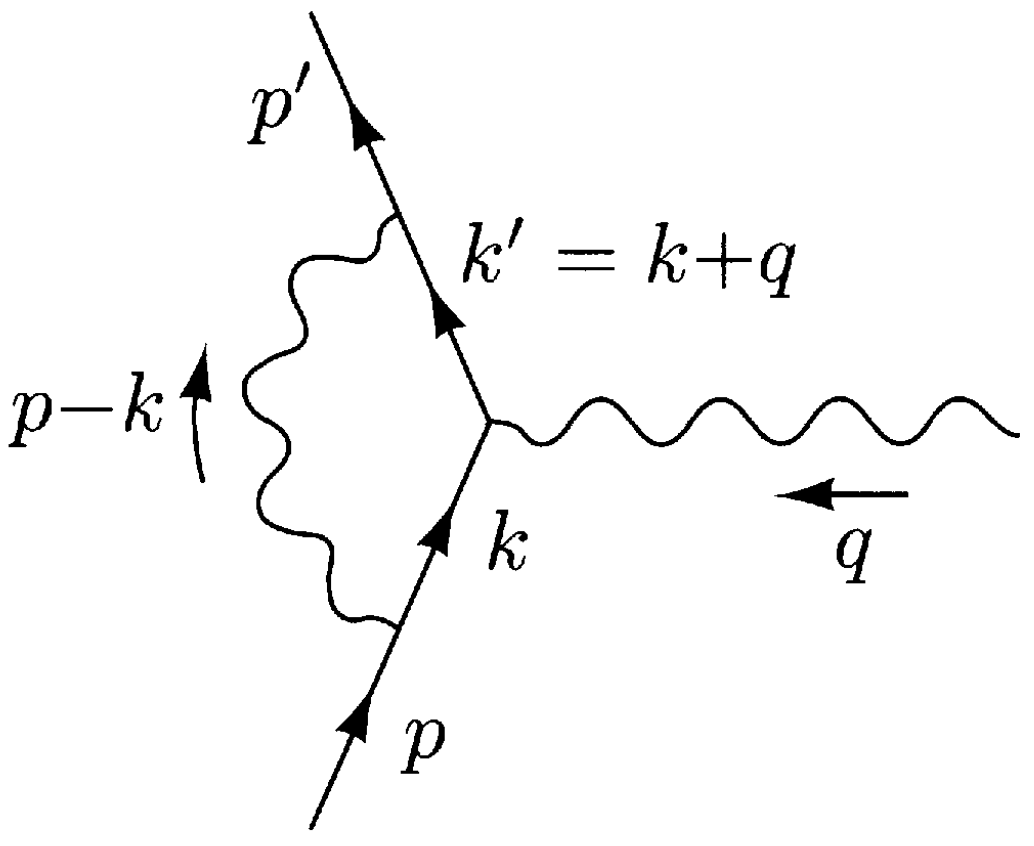
\includegraphics[width=0.3\linewidth]{pics/QED-3.png}
\end{equation*}
There is 4 electron propagator, 2 photon propagator, and 3 vertices.
Consider the perturbative expansion:
\begin{equation*}
	\frac{\delta^3}{i\delta J \delta\bar\eta \delta\eta}\frac{1}{2!}
	\left(\frac{-e\gamma^\mu_{\alpha\beta}\delta^3}{\delta J^\mu \delta\eta_{\alpha} \delta\bar\eta_{\beta}}\right)^3 
	\frac{1}{2!}\left(-i \bar\eta_{\alpha} D_F^{\alpha\beta} \eta_{\beta} \right)^4 
	\frac{1}{2!}\left(-\frac{i}{2} J^\mu \Pi_{\mu\nu} J^{\nu} \right)^2.
\end{equation*}
There is not symmetry factor, and an additional $-i$ factor. 
The total coefficient is $-ie^3$. 

Then consider the tensor contraction
\begin{equation*}
	D_F^{\alpha\gamma} \gamma^\nu_{\gamma\rho} D_F^{\rho\sigma} \gamma^\zeta_{\sigma\tau} D_F^{\tau\eta} \gamma^\lambda_{\eta\xi} D_F^{\xi\beta} \Pi_{\nu\lambda} \Pi_{\mu\zeta}.
\end{equation*}

The vertex correction is:
\begin{equation*}
	iV_3(q,p,p') = [iD_F(p)][iD_F(p')][i\Pi^{\mu\nu}(q)][-ie\Gamma^\nu(q,p,p')] 
\end{equation*}
where
\begin{equation}
	i\Gamma^\mu(q,p,p')
	= -e^2 \int\frac{d^4 k}{(2\pi)^4} 
	\Pi_{\nu\lambda}(p-k) 
	\gamma^\nu D_F(k') \gamma^\mu D_F(k) \gamma^\lambda.
	\label{eq:QED-loop-vertex}
\end{equation}
\end{framedexpl}

\begin{framedexpl}[Counter Terms]
Consider the counter term in the diagram
\begin{equation*}
	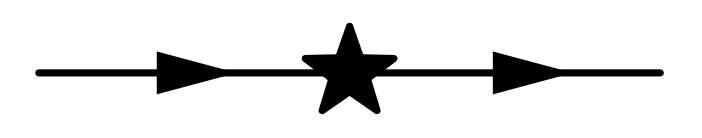
\includegraphics[width=0.25\linewidth]{pics/QED-ct-1.png}
\end{equation*}
The perturbative expansion is
\begin{equation*}
	iD_F^{\mathrm{(ct)}} \sim \frac{\delta^2}{\delta\bar\eta \delta\eta}
	i(\delta_{\psi}\gamma^\mu_{\alpha\beta}k_\mu-\delta_m \mathbb{I}_{\alpha\beta})\frac{\delta^2}{\delta\eta_{\alpha} \delta\bar\eta_{\beta}}
	\frac{1}{2!}\left(-i \bar\eta_{\alpha} D_F^{\alpha\beta} \eta_{\beta} \right)^2.
\end{equation*}
The contribution to the electron self energy is
\begin{equation*}
	\delta_{\psi}\cancel{k}-\delta_m m_R.
\end{equation*}
Similarly, the digram
\begin{equation*}
	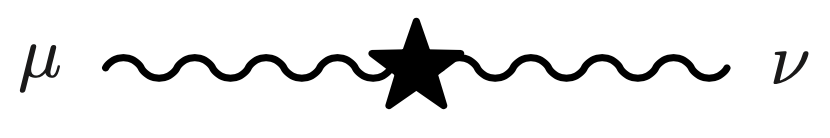
\includegraphics[width=0.25\linewidth]{pics/QED-ct-2.png}
\end{equation*}
contribute to the photon self energy with term
\begin{equation*}
	\delta_A [-p^2 g^{\mu\nu} + (1-\xi)p^\mu p^\nu],
\end{equation*}
and the diagram
\begin{equation*}
	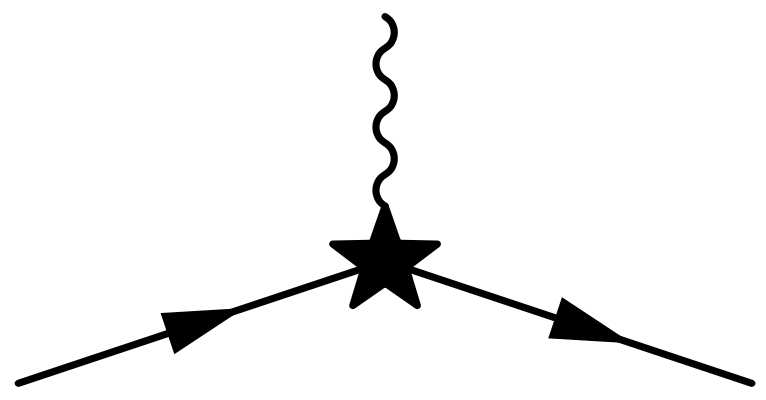
\includegraphics[width=0.2\linewidth]{pics/QED-ct-3.png}
\end{equation*}
contribute to the vertex with term
\begin{equation*}
	\delta_e \gamma^\mu.
\end{equation*}
\end{framedexpl}



\section{Loop Correction}
In this section, we consider the QED in ($d=4-\epsilon$) dimensional space-time.
\subsection{Electron Propagator}
Consider the one-loop correction to the electron propagator, where the self energy (\ref{eq:QED-ele-loop-prop}) is
\begin{equation}
\begin{aligned}
	i\Sigma(p^2)
	&= e^2\tilde{\mu}^{\epsilon}\int\frac{d^d k}{(2\pi)^d} \Pi_{\mu\nu}(p-k) \left[\gamma^\mu D_F(k) \gamma^\nu \right]_{\alpha\beta} \\
	&= -e^2\tilde{\mu}^{\epsilon}\int\frac{d^d k}{(2\pi)^d}\frac{\gamma^\mu(\cancel{k}+m)\gamma_\mu}{(p-k)^2(k^2-m^2)}.
\end{aligned}
\end{equation}
The nominator can be simplified using the \texttt{FeynCalc} Package:
\begin{lstlisting}[style=mathematicaFrameTB]
(*load FeynCalc Package*)
<< FeynCalc`

(*simplify the gamma expression*)
Contract[GA[\[Mu]].(GS[k]+m).GA[\[Mu]]]//DiracSimplify	
\end{lstlisting}
The result is
\begin{equation*}
	4 m-2\cancel{k}.
\end{equation*}
The denominator can be simplify using the Feynman parameter:
\begin{equation*}
	\frac{1}{(p-k)^2(k^2-m^2)} = \int_0^1 \frac{dx}{\left[(k-b)^2-D\right]^2}
\end{equation*}
where $b$ and $D$ can be calculated by
\begin{lstlisting}[style=mathematicaFrameTB]
A1=(k-p)^2;
A2=k^2-m^2;
{c,b,a}=CoefficientList[x*A1+(1-x)*A2,{k}];
-b/2
-c+b^2/(4*a)//Simplify
\end{lstlisting}
The result is
\begin{equation*}
	b = p x,\ 
	D = (1-x)(m^2-p^2 x).
\end{equation*}
Shift $k \rightarrow k + px$, the self energy becomes:
\begin{equation}
\begin{aligned}
	i\Sigma(p^2)
	&= 2e^2\tilde{\mu}^{\epsilon} 
		\int_0^1 (x\cancel{p}-2m)dx 
		\int \frac{d^d k}{(2\pi)^d} 
		\frac{1}{(k^2-D)^2} \\
	&= i\frac{2e^2 \tilde{\mu}^{\epsilon}\Omega_d}{(2\pi)^d}
		\int_0^1 (x\cancel{p}-2m)dx
		\int \frac{k^{d-1} dk}{(k^2+D)^2}.
\end{aligned}
\end{equation}
The regularization procedure
\begin{lstlisting}[style=mathematicaFrameTB]
omg=(2*Pi^(d/2))/(Gamma[d/2]);
cof=2*e^2*\[Mu]^(4-d)*omg/(2*Pi)^d;
int=cof*Integrate[q^(d-1)/(q^2+D)^2,{q,0,Infinity}][[1]];
map={e->Sqrt[4*Pi*\[Alpha]],EulerGamma->Subscript[\[Gamma],E]};
ans=Series[int/.{d->4-\[Epsilon]},{\[Epsilon],0,0}];
ans/.map//Simplify
\end{lstlisting}
The result is ($\mu^2 = 4\pi \tilde\mu^2 e^{-\gamma_E}$)
\begin{equation}
	\Sigma(p^2) = \frac{e_R^2}{8\pi^2}\int_0^1 dx(x\cancel{p}-2m_R)\left[\frac{2}{\epsilon}+\ln\left(\frac{\mu^2}{D}\right)\right].
\end{equation}
The infinity comes from
\begin{equation*}
	\frac{e_R^2}{4\pi^2\epsilon}\int_0^1 dx(x\cancel{p}-2m_R)
	= \frac{e_R^2}{8\pi^2\epsilon}\cancel{p} - \frac{e_R^2}{2\pi^2\epsilon}m_R.
\end{equation*}
Using the $\overline{\mathrm{MS}}$ subtraction scheme, we choose
\begin{equation}
	\delta_{\psi} = -\frac{e_R^2}{8\pi^2\epsilon},\ 
	\delta_m = -\frac{e_R^2}{2\pi^2\epsilon},
\end{equation}
and the self energy is
\begin{equation}
\begin{aligned}
	\Sigma(p^2) 
	&= \frac{e_R^2}{8\pi^2}\int_0^1 dx(x\cancel{p}-2m_R)\ln\left[\frac{\mu^2}{(1-x)(m_R^2-p^2 x)}\right] \\
	&= \frac{e_R^2}{8\pi^2}(\cancel{p}-4m_R)\ln\left(\frac{\mu}{m_R}\right)-\int_0^1 dx \ln\left[(1-x)\left(1-\frac{p^2x}{m_R^2}\right)\right].
\end{aligned}
\end{equation}



\subsection{Photon Self-energy}
Consider the one-loop correction to the photon propagator, where the self energy (\ref{eq:QED-photon-loop-prop}) is
\begin{equation}
	i \Sigma^{\mu\nu}
	= -e^2\tilde{\mu}^{\epsilon} \int\frac{d^d k}{(2\pi)^d} 
	\frac{\mathrm{Tr}\left[\gamma^\mu D_F(k-p) \gamma^\nu D_F(k) \right]}{(k^2-m^2)[(p-k)^2-m^2]}.
\end{equation}
The Dirac trace and Feynman parameter is calculated by
\begin{lstlisting}[style=mathematicaFrameTB]
(*Dirac trace*)
DiracTrace[GA[\[Mu]].(GS[k-p]+m).GA[\[Nu]].(GS[k]+m)]//DiracSimplify

(*Feynman paramater*)
A1=k^2-m^2;
A2=(k-p)^2-m^2;
{c,b,a}=CoefficientList[x*A1+(1-x)*A2,{k}];
-b/2
-c+b^2/(4*a)//Simplify
\end{lstlisting}
The nominator is
\begin{equation*}
	4 \left[g^{\mu\nu} \left(k\cdot p-{k}^2+m^2\right)+ 2k^\mu k^\nu - k^\mu p^\nu - p^\mu k^\nu \right]
\end{equation*}
The denominator is:
\begin{equation*}
	\frac{1}{(k^2-m^2)[(p-k)^2-m^2]}
	= \frac{1}{\left\{[k-p(1-x)]^2-[m^2+p^2 x(x-1)]\right\}^2}
\end{equation*}
Let $D=m^2-p^2 x(1-x)$, shift $k \rightarrow k + p(1-x)$, and drop all $p^\mu$ linear term,\footnote{The Ward identity requires that the $p^\mu$ term in the propagator do not contribute to any scattering process.} the result is
\begin{equation}
	i\Sigma^{\mu \nu}= -4 e^{2}\tilde{\mu}^{\epsilon} \int_0^1 dx
		\int \frac{d^{d} k}{(2 \pi)^{d}}  \frac{2 k^{\mu} k^{\nu}-g^{\mu \nu}\left[k^{2}-x(1-x) p^{2}-m^{2}\right]}{\left[k^{2}-D\right]^{2}}
\end{equation}
The self-energy $i\Sigma^\mu \propto g^{\mu\nu}$, we can make the substitution
\begin{equation*}
	k^\mu k^\nu \rightarrow \frac{1}{d} k^2 g^{\mu\nu}.
\end{equation*}
We then need to consider the integral
\begin{equation*}
\begin{aligned}
	iI(x) &= 4e^2\tilde{\mu}^{\epsilon} \int\frac{d^d k}{(2 \pi)^{d}}  
		\frac{(1-\frac{2}{d})k^{2}-x(1-x) p^{2}-m^{2}}{\left[k^{2}-D\right]^{2}}, \\
	I(x) &= -\frac{4e^2\tilde{\mu}^{\epsilon} \Omega_d }{(2\pi)^d}
		\int k^{d-1} dk \frac{(1-\frac{2}{d})k^{2}+x(1-x) p^{2}+m^{2}}{\left[k^{2}+D\right]^{2}}.
\end{aligned}
\end{equation*}
The regulation is carried out by the following code:
\begin{lstlisting}[style=mathematicaFrameTB]
omg=(2*Pi^(d/2))/(Gamma[d/2]);
cof=-4*e^2*\[Mu]^(4-d)*omg/(2*Pi)^d;
den=q^(d-1)*((1-2/d)q^2+x*(1-x)p^2+m^2);
int=cof*Integrate[den/(q^2+D)^2,{q,0,Infinity}][[1]];
map={EulerGamma->Subscript[\[Gamma],E],D->m^2-p^2*x*(1-x)};
ans=Series[int/.{d->4-\[Epsilon]},{\[Epsilon], 0, 0}];
ans/.map//Simplify
\end{lstlisting}
The result is
\begin{equation}
	\Sigma^{\mu\nu}(p^2) 
	= -\frac{e_R^2 p^2 g^{\mu\nu}}{2\pi^2} \int_0^1 dx\ x(1-x)
	\left[\frac{2}{\epsilon}+\ln\left(\frac{\mu^2}{m_R^2-p^2 x(1-x)}\right)\right]
\end{equation}
The divergent part is
\begin{equation*}
	-\frac{e_R^2 p^2 g^{\mu\nu}}{\pi^2 \epsilon} \int_0^1 dx\ x(1-x)
	= -\frac{e_R^2 p^2 g^{\mu\nu}}{6\pi^2 \epsilon}.
\end{equation*}
The counter term coefficient is
\begin{equation}
	\delta_A = -\frac{e_R^2}{6\pi^2 \epsilon}.
\end{equation}
The photon self-energy is then
\begin{equation}
\begin{aligned}
	\Sigma^{\mu\nu}(p^2) 
	&= -\frac{e_R^2 p^2 g^{\mu\nu}}{2\pi^2} \int_0^1 dx\ x(1-x)
	\ln\left[\frac{\mu^2}{m_R^2-p^2 x(1-x)}\right] \\
	&= -\frac{e_R^2 p^2 g^{\mu\nu}}{12\pi^2} \ln\left(\frac{\mu}{m}\right)
	 + \frac{e_R^2 p^2 g^{\mu\nu}}{2\pi^2}\int_0^{1} dx\ x(1-x) \ln\left[1-\frac{p^2}{m_R^2}x(1-x)\right].
\end{aligned}
\end{equation}


\subsection{Vertex Correction}
Consider the loop correction (\ref{eq:QED-loop-vertex}):
\begin{equation}
	i \Gamma^\mu(p,q_1,q_2)
	= e^2\tilde{\mu}^{\epsilon} \int\frac{d^4 k}{(2\pi)^4} 
	\frac{\gamma^\nu(\cancel{k}'+m)\gamma^\mu (\cancel{k}+m)\gamma_\nu}{(k^2-m^2)(k'^2-m^2)(p-k)^2}.
\end{equation}
Using the following code
\begin{lstlisting}[style=mathematicaFrameTB]
(*numerator*)
den=Contract[GA[\[Nu]].(GS[kp]+m).GA[\[Mu]].(GS[k]+m).GA[\[Nu]]];
DiracSimplify[den]

(*Feynman parameter*)
A1=k^2-m^2;
A2=(k+q)^2-m^2;
A3=(p-k)^2;
{c,b,a}=CoefficientList[x*A1+y*A2+z*A3,{k}];
-b/2//Simplify
-c+b^2/4//Simplify
\end{lstlisting}
The numerator is
\begin{equation*}
	-2\cancel{k}\gamma^\mu\cancel{k}'-2m^2\gamma^\mu + 4m(k + k')^\mu.
\end{equation*}
The denominator is
\begin{equation*}
	\int \frac{dF_3}{[(k+yq-zp)^2-D]^3},
\end{equation*}
where 
\begin{equation*}
\begin{aligned}
	D &= (x+y)m^2 - z(1-z)p^2- y(1-y)q^2-2yzpq \\
	&=(x+y)m^2 - xy q^2- yz p'^2 - xz p^2.
\end{aligned}
\end{equation*}
Shift $k^\mu \rightarrow k^\mu + z q_1^\mu - y p^\mu$, throw away all terms with linear $k^\mu$, and replace $k^\mu k^\nu$ with $\frac{1}{d}k^2 g^{\mu\nu}$, the result is
\begin{equation*}
	\frac{4}{d}k^2\gamma^\mu  -2(-y \cancel{q}+z \cancel{p}) \gamma^{\mu}[(1-y) \cancel q+z \cancel p] +4 m^{2} \gamma^{\mu}-2 m\left[(1-2 y) q^{\mu}+2 z p^{\mu}\right].
\end{equation*}
Note that only the quadratic term is divergent. 
\begin{equation*}
	\Gamma^\mu(p,q_1,q_2) = -i\frac{4e^2\tilde{\mu}^{\epsilon} \gamma^\mu}{d}  \int dF_3 \int \frac{d^dk}{(2\pi)^d} \frac{k^2}{(k^2-D)^3} + \delta\Gamma^\mu(p,q_1,q_2).
\end{equation*}
where $\delta \Gamma^\mu$ stores all the finite part
\begin{equation*}
\begin{aligned}
	& \delta\Gamma^\mu(p,q_1,q_2) \\
	=& \int \frac{e^2 k^3 dk dF_3}{(2\pi)^2(k^2+D)^3} \left\{(-y \cancel{q}+z \cancel{p}) \gamma^{\mu}[(1-y) \cancel q+z \cancel p] -2 m^{2} \gamma^{\mu}+ m\left[(1-2 y) q^{\mu}+2 z p^{\mu}\right]\right\}.
\end{aligned}
\end{equation*}
The divergent part is
\begin{equation*}
	\frac{4 e^2\tilde{\mu}^{\epsilon} \Omega_d \gamma^\mu}{d(2\pi)^d}\int dF_3 \int \frac{k^{d+1}dk}{(k^2+D)^3}
	= \frac{e_R^2}{16\pi^2} \gamma^\mu \int dF_3 \left[\frac{2}{\epsilon}+\ln\left(\frac{\mu^2}{D}\right)\right].
\end{equation*}
Using the $\overline{\mathrm{MS}}$ scheme, the coefficient of the counter term is
\begin{equation}
	\delta_e = -\frac{e_R^2}{8\pi^2\epsilon}.
\end{equation}


\subsection{Renormalization Group}
In summery, the renormalization factors are
\begin{equation}
\begin{aligned}
	Z_\psi &= 1 -\frac{e_R^2}{8\pi^2\epsilon} + O(e_R^3), \\
	Z_A &= 1 - \frac{e_R^2}{6\pi^2 \epsilon} + O(e_R^3), \\
	Z_m &= 1 - \frac{e_R^2}{2\pi^2\epsilon} + O(e_R^3), \\
	Z_e &= 1 - \frac{e_R^2}{8\pi^2\epsilon} + O(e_R^3),
\end{aligned}
\end{equation}
which means
\begin{equation}
\begin{aligned}
	\frac{d\ln Z_\phi}{d e_R} &= -\frac{e_R}{4\pi^2 \epsilon} + O(e_R^2), \\
	\frac{d\ln Z_A}{d e_R} &= -\frac{e_R}{3\pi^2 \epsilon} + O(e_R^2), \\
	\frac{d\ln Z_m}{d e_R} &= -\frac{e_R}{\pi^2 \epsilon} + O(e_R^2), \\
	\frac{d\ln Z_e}{d e_R} &= -\frac{e_R}{4\pi^2 \epsilon} + O(e_R^2).
\end{aligned}
\end{equation}
The bare parameters are
\begin{equation}
\begin{aligned}
	\psi_0 &= Z_\psi^{1/2}\psi_R, \\
	A_0 &= Z_A^{1/2} A_R, \\
	m_0 &= Z_m Z_\psi^{-1} m_R, \\
	e_0 &= Z_e Z_\psi^{-1} Z_A^{-1/2} e_R \tilde{\mu}^{\epsilon/2}. 
\end{aligned}
\end{equation}
The RG equation for $e_0$ is
\begin{equation}
	\frac{d\ln e_0}{d\ln \mu}
	= \left(\frac{\ln Z_e}{d e_R} - \frac{\ln Z_\psi}{d e_R} - \frac{1}{2} \frac{\ln Z_A}{d e_R} + \frac{1}{e_R} \right)\frac{de_R}{d\ln \mu} + \frac{\epsilon}{2} = 0.
\end{equation}
The beta function is
\begin{equation}
	\beta(e_R) = \frac{de_R}{d\ln \mu} = -\frac{\epsilon}{2}e_R + \frac{e_R^3}{12\pi^2} + O(e_R^4).
\end{equation}
The RG equation for $m_0$ is
\begin{equation}
	\frac{d\ln m_0}{d\ln \mu}
	= \left(\frac{\ln Z_m}{d e_R} - \frac{\ln Z_\psi}{d e_R}\right)\frac{de_R}{d\ln \mu} + + \frac{1}{m_R}\frac{d m_R}{d\ln\mu} = 0.
\end{equation}
The anomalous dimension of mass is
\begin{equation}
	\gamma_m = \frac{d \ln m_R}{d\ln\mu} = -\frac{3e_R^2}{8\pi^2} + O(e_R^3).
\end{equation}




\chapter{Non-relativistic Quantum Field Theory}
A general non-relativistic field theory is described by the action (with repeated indices automatically summed):
\begin{equation}
\begin{aligned}
	S &= S_0 + S_{\mathrm{int}} = \int dt \int d^d x \mathcal{L}_0 + \int dt\ \mathcal{V}_{\mathrm{int}}, \\
	\mathcal{L}_0 &= \bar\psi_a(x) (i\delta_{ab}\partial_t-\hat H_{ab})\psi_b(x).
\end{aligned}
\end{equation}
where the field operator $\psi(x)$ can be bosonic or fermionic, which is denoted by a number $\zeta=\pm 1$, and $\mathcal{V}_{\mathrm{int}}$ is the interaction Lagrangian.
A general interaction has the form
\begin{equation}
	\mathcal{V}_{\mathrm{int}} = \sum_{abcd}\int \prod_{i=1}^4 d^d x_i \ \bar\psi_{c}(x_3)\bar\psi_{d}(x_4) V_{abcd}(x_1,x_2,x_3,x_4) \psi_{b}(x_2)\psi_{a}(x_1).
\end{equation}
Note that the classical equation of motion for the free field satisfies the Schr\"{o}dinger equation:
\begin{equation}
	\partial_\mu \frac{\partial \mathcal L_0}{\partial(\partial_\mu \bar\psi_a(x))} - \frac{\partial \mathcal L_0}{\partial\bar{\psi}_a(x)} 
	= - i\partial_t \psi_a(x) + \hat H_{ab}\psi_b(x) = 0.
\end{equation}

We are mostly work with finite system size $L^d$ with UV cutoff $\Lambda = 2\pi/a$ (where $a$ is the lattice spacing, and $L = Na$). The spatial Fourier transformation is
\begin{equation}
	\tilde{\psi}_a(k) = \int_{L^d} d^dx e^{-i k \cdot x}\psi_a(x), \quad
	\psi_a(x) = \frac{1}{L^d}\sum_{k} e^{i k \cdot x}\tilde{\psi}_a(k).
\end{equation}
For the finite size, the momentum is discretized: $k = 2\pi n_k/L$, $n_k \in \mathbb Z$.
The summation in the thermodynamic limit becomes the integral:
\begin{equation}
	\frac{1}{L^d}\sum_k \longrightarrow \int_{|k|<\Lambda} \frac{d^dk}{(2\pi)^d}.
\end{equation}
In the momentum space, the free theory can be simplified:
\begin{equation}
	S_0 = \int dt \int \frac{d^d k}{(2\pi)^d} \tilde{\bar\psi}_a(k) [i\partial_t-\varepsilon_a(k)]\tilde{\psi}_a(k).
\end{equation}
The interaction in the momentum space is described by the vertex function:
\begin{equation}
	\tilde V_{abcd}(k_1,k_2,k_3,k_4)
	= \int \prod_{i=1}^4 d^d x_i e^{i(k_1x_1+k_2x_2-k_3x_3-k_4x_4)} V_{abcd}(x_1,x_2,x_3,x_4).
\end{equation}
Because of the momentum conservation, the vertex will contain a delta function factor.

Consider the Coulomb repulsive potential $e^2/r$, in the field theory formalism, the coefficient $V_{abcd}(x_1,x_2,x_3,x_4)$ is
\begin{equation}
\begin{aligned}
	\frac{V(x_1-x_2)}{2!2!}\left[\delta_{ac}\delta_{bd}\delta^{(3)}(x_1-x_3)\delta^{(3)}(x_2-x_4) - \delta_{ad}\delta_{bc}\delta^{(3)}(x_1-x_4)\delta^{(3)}(x_2-x_3)\right],
\end{aligned}
\end{equation}
where the factor $\frac{1}{2!2!}$ is the symmetry from interchanging the fermion fields.
In momentum space:
\begin{equation}
	V_{abab}(k_1,k_2,k_3+q,k_4-q) = \frac{1}{2!2!} V_{\mathrm{Coul}}(q),
\end{equation}
where the Coulomb potential in the momentum space is
\begin{equation}
\begin{aligned}
	V_{\mathrm{Coul}}(q) 
	&=  \lim_{\alpha\rightarrow0}e^{2}\int_{0}^{\infty}dr\ 2\pi r^{2} \int_{-1}^{+1}d\left(\cos\theta\right)\frac{e^{-iqr\cos\theta-\alpha r}}{r} \\
	&=  \lim_{\alpha\rightarrow0}\frac{2\pi e^{2}}{iq}\int_{0}^{\infty}dr\left(e^{iqr-\alpha r}-e^{-iqr-\alpha r}\right)\\
 	&=  \lim_{\alpha\rightarrow0}\frac{4\pi e^{2}}{q^{2}+\alpha^{2}}
	=  \frac{4\pi e^{2}}{q^{2}}.
\end{aligned}
\end{equation}



\section{Finite Temperature Field Theory}

The original real-time partition function is defined as\footnote{As with the relativistic case, we introduce an auxiliary source $J$, which is bosonic/fermionic if the field $\psi$ is bosonic/fermionic.
}
\begin{equation}
	Z[J] = \int D[\bar\psi,\psi] \exp\left\{i\int dt \int d^dx \left[\mathcal{L}+\bar{J}_a(x)\psi_a(x)+\bar{\psi}_a(x)J_a(x)\right]\right\}.
\end{equation}
For finite-temperature field theory, after making the wick rotation ($t \rightarrow -i\tau$), the partition function for a generic non-relativistic lattice theory is:
\begin{equation}
	Z[J] = \int D[\bar\psi,\psi] e^{-S[\bar\psi,\psi]+\bar{J}\cdot\psi+\bar{\psi}\cdot J},
\end{equation}
where the action is
\begin{equation}
	S = \int_0^\beta d\tau \left[\int d^dx\ \bar\psi_a(x) (\delta_{ab}\partial_\tau+\hat H_{ab})\psi_b(x) + \mathcal{V}_{\mathrm{int}}\right].
\end{equation}
The Fourier transformation on the imaginary time domain is defined as:
\begin{equation}
	\tilde\psi(\omega_n) = \int_0^\beta d\tau e^{i\omega_n\tau} \psi(\tau),\quad
	\psi(\tau) = \frac{1}{\beta}\sum_{\omega_n} e^{-i\omega_n\tau} \tilde\psi(\omega_n).
\end{equation}
Under such convention, in the thermodynamic limit and zero-temperature limit, the spatial-temporal Fourier transformation agrees with the relativistic case (up to a Wick rotation).



\subsection{Free Field Theory}
We first consider the action of free field
\begin{equation}
	S_0 = \int_0^\beta d\tau \int d^dx\ \bar\psi_a(x) (\delta_{ab}\partial_\tau+\hat H_{ab})\psi_b(x).
\end{equation}
The Fourier transformation
\begin{equation}
	S_0 = \frac{1}{\beta}\sum_{\omega_n} \int_{\Lambda} \frac{d^dk}{(2\pi)^d}
	\tilde{\bar{\psi}}_a(k,\omega_n)\left[-i\omega_n + \tilde{H}_{ab}(k)\right]\tilde{\psi}_b(k,\omega_n).
\end{equation}
The partition function with source is
\begin{equation}
	\frac{Z_0[J]}{Z_0[0]} = \exp\left[-\frac{1}{\beta}\sum_{\omega_n} \int_{\Lambda} \frac{d^dk}{(2\pi)^d}\tilde{\bar J}_a(k,\omega_n) \tilde{G}_{ab}(k,\omega_n) \tilde{J}_b(k,\omega_n) \right],
\end{equation}
where the Green's function is
\begin{equation}
	\tilde{G}_{ab}(k,\omega_n) = \left[\frac{1}{i\omega_n - \tilde{H}(k)}\right]_{ab}.
\end{equation}

\begin{framedrmk}[Obtaining the Partition Function]
Unlike the relativistic case, the value of the value of partition function without source $Z_0[0]$ is related to the free energy.
We can express it formally as
\begin{equation*}
	Z_0[0]= \left[\det (-G_{ab})^{-1}\right]^{-\zeta}.
\end{equation*}
To get the correct dimensionality, we set the determinant as
\begin{equation*}
	Z_0[0] \equiv \prod_{k,\omega_n}\left\{\beta \det\left[-i\omega_n+\tilde{H}(k)\right]\right\}^{-\zeta}.
\end{equation*}
Thus the free energy is
\begin{equation}
	F = -\frac{1}{\beta} \ln Z_0
	= \zeta \sum_{k,\omega_n} \ln\left\{\beta\det\left[-i\omega_n+\tilde{H}(k)\right]\right\}.
\end{equation}
\end{framedrmk}

\subsection{Matsubara Summation}
Now consider the summation on Matsubara frequency:
\begin{equation}
	\sum_{\omega_n} f(\omega_n) = 
	\begin{cases}
		\sum_n f(\frac{2n\pi}{\beta}) & \mathrm{bosonic} \\
		\sum_n f(\frac{(2n+1)\pi}{\beta}) & \mathrm{fermionic}
	\end{cases}.
\end{equation}
The frequency is capture by the singularities of the density function of the states:
\begin{equation}
	\rho(z) = \begin{cases}
		\frac{1}{\exp(\beta z)-1} & \mathrm{bosonic} \\
		\frac{1}{\exp(\beta z)+1} & \mathrm{fermionic}
	\end{cases}.
\end{equation}
The residue on imaginary frequency $i\omega_n$ is alway $\frac{1}{\beta}$. In this way, the summation is:
\begin{equation}
	\frac{1}{\beta}\sum_{\omega_n} f(i\omega_n) 
	= \frac{1}{2\pi i} \oint \rho(z)f(z)
	= -\sum_{k} \mathrm{Res}\ \rho(z)f(z)|_{z=z_k}.
\end{equation}

\subsubsection*{Summation of Green's function}
Consider the frequency summation for the correlation function:
\begin{equation}
	\frac{1}{\beta}\sum_{\omega_n} \tilde{G}_0(k) 
	= \frac{1}{\beta}\sum_{\omega_n}\frac{1}{i\omega_n-E_{p}}
	= -\mathrm{Res} \left. \frac{\rho(z)}{z-E_{p}}\right|_{z=E_{p}}
	= \rho(E_{p}).
\end{equation}


\subsubsection*{Summation of Green's function}
Consider the frequency summation for the correlation function:
\begin{equation}
	\sum_{\omega_n} \langle\bar\psi_{\vec p,\omega_n}\psi_{\vec p, \omega_n}\rangle = \frac{1}{\beta}\sum_{\omega_n}\frac{1}{-i\omega_n+\epsilon_{\vec p}}
	= \mathrm{Res} \left. \frac{\rho(z)}{z-\epsilon_{\vec p}}\right|_{z-\epsilon_{\vec p}}
	= \rho(\epsilon_{\vec p}).
\end{equation}

\subsubsection*{Free Energy Summation}
Consider the free energy
\begin{equation}
	F = -\frac{1}{\beta}\ln Z 
	= -\frac{1}{\beta}\sum_{\omega_n}\ln[\beta(-i\omega_n+E_{\vec p})]
	= \frac{1}{2\pi i} \oint dz \rho(z)\ln[\beta(\xi - z)].
\end{equation}
To calculate the summation, we consider the line integral along the loop:
\begin{equation*}
	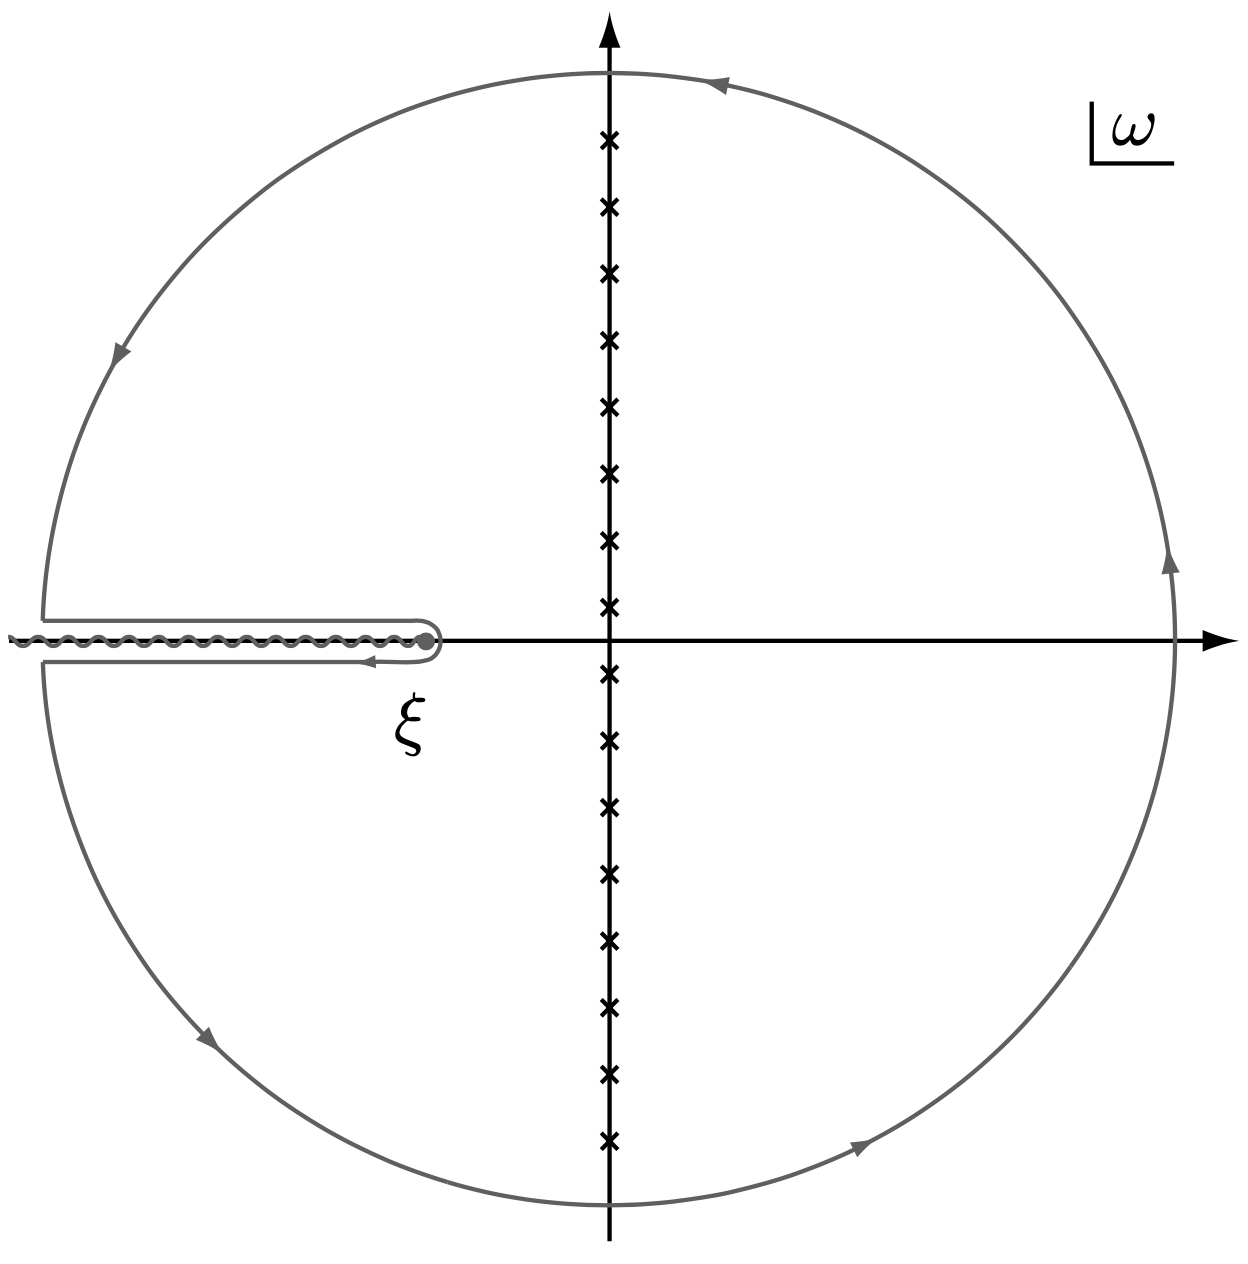
\includegraphics[width=0.25\linewidth]{pics/FqSum.png}
\end{equation*}
The free energy is
\begin{equation}
\begin{aligned}
	F &= \frac{1}{2\pi i}\int_{-\infty}^\infty dx \rho(x)\ln\left(\frac{\xi-x-i\epsilon}{\xi-x+i\epsilon}\right) \\
	&= \frac{-\zeta}{2\pi i\beta} \int_{-\infty}^{\infty}dx \ln(1-\zeta e^{-\beta z})\left(\frac{1}{x+i\epsilon-\xi}-\frac{1}{x-i\epsilon-\xi}\right),
\end{aligned}
\end{equation}
where we integrate the expression by part, noticing that
\begin{equation}
	\frac{d}{dz} \frac{\zeta}{\beta} \ln(1-\zeta e^{-\beta z}) = \frac{1}{e^{\beta z}-\zeta} = \rho(z)
\end{equation}
Using the identity
\begin{equation*}
	\lim_{\epsilon\rightarrow 0^+} \frac{1}{x+i\epsilon} = -i\pi\delta(x) + \mathcal{P}\frac{1}{x},
\end{equation*}
the above expression can be simplified to
\begin{equation}
	F = \frac{\zeta}{\beta} \ln(1-\zeta e^{-\beta\zeta}).
\end{equation}


\section{Fermi Liquid Theory}
In this section, we are considering the system of weakly interacting Fermi gas.
To be specific, we consider the lattice Hamiltonian:
\begin{equation}\label{eq:FL-gen-ham}
	H = -\frac{1}{2}\sum_{\langle i,j \rangle} (c_i^\dagger c_{j} + c_{j}^\dagger c_i) + \mu\sum_i c_i^\dagger c_i + \sum_{i,j,k,l} u_{ijkl} c_i^\dagger c_j^\dagger c_k c_l.
\end{equation}
In the following, we investigate the effective field theory near the Fermi surface.
We discuss the RG flow of the couplings (mainly for two dimensional system).
Then we carry out the perturbative calculation for the correlation functions. 

\subsection{Effective Field Theory for Interacting Fermi Systems}
The low-energy manifold is an annulus of thickness $2 \Lambda$ symmetrically situated with respect to the Fermi circle $K=K_{\mathrm{F}}$.
The dispersion for the free lattice model is
\begin{equation}
	E(\bm K) = -\cos K_x - \cos K_y \simeq -2 + \frac{\bm K^2}{2}.
\end{equation}
For a given chemical potential $\mu$, the Fermi circle is $K_F = \sqrt{2m\mu}$, we can linearize the dispersion near the Fermi surface:
\begin{equation}
	E(\bm K) = \frac{\bm K^2-K_F^2}{2m} \simeq \frac{K_F}{m}k \equiv v_F k, \quad
	k\equiv |K|-K_F
\end{equation}
The partition function is:
\begin{equation}
	Z_0 = \sum_\theta \sum_{|k|<\Lambda}\int D\left[\bar\psi(k,\theta,\omega),\psi(k,\theta,\omega)\right] e^{-S_0},
\end{equation}
where the free field action is:\footnote{A factor of $K_{\mathrm{F}}$ has been absorbed in the field.}
\begin{equation}
	S_0 = \int \frac{d\theta}{2\pi} \int^\Lambda_{-\Lambda}\frac{dk}{2\pi} \int^\infty_{-\infty}\frac{d\omega}{2\pi} \bar\psi(k,\theta,\omega)(-i\omega+v_F k)\psi(k,\theta,\omega).
\end{equation}
Consider the quartic interaction
\begin{equation}
	\delta S_4 = \frac{1}{4}\int_{\bm K,\theta,\omega} \bar\psi(4)\bar\psi(3)\psi(2)\psi(1)u(4,3,2,1)
\end{equation}
where we eliminate one of the four sets of variables, say, the one numbered 4, by integrating them against the delta functions:
\begin{equation}
	\int_{K,\theta,\omega}
	=\prod_{i=1}^{3} \int_{0}^{2 \pi} \frac{d \theta_{i}}{2 \pi} \int_{-\Lambda}^{\Lambda} \frac{d k_{i}}{2 \pi} \int_{-\infty}^{\infty} \frac{d \omega_{i}}{2 \pi} \theta\left(\Lambda-\left|k_{4}\right|\right), \quad 
	k_4 = |\bm K_4|-K_F.
\end{equation}
The $\omega$ integral is easy: since all $\omega$'s are allowed, the condition $\omega_4=\omega_1+\omega_2-\omega_3$ is always satisfied for any choice of the first three frequencies. 
The same would be true for the momenta if all momenta were allowed. 
But they are not; they are required to lie within the annulus of thickness $2\Lambda$ around the Fermi circle. 
Consequently, if one freely chooses the first three momenta from the annulus, the fourth could have a length as large as $3K_F$. 
The role of $\delta(\Lambda-|k_4|)$ is to prevent exactly this.

\subsubsection*{Momentum Constraint}
Note that $k_4$ can be expressed as
\begin{equation}
	k_4 = |(K_F+k_1)\bm \Omega_1+(K_f+k_2)\bm \Omega_2-(K_F+k_3)\bm \Omega_3|-K_F.
\end{equation}
When doing RG towards the Fermi surface, the integral measure will not preserve the preserve the original form.
The situation is clearly is we use a smooth cutoff
\begin{equation}
	\theta(\Lambda-|k_4|) \rightarrow e^{-|k_4|/\Lambda},
\end{equation}
and define $\Delta\equiv \bm \Omega_1+\bm \Omega_2-\bm \Omega_3$, $k_4$ in this way behaves as
\begin{equation}
	k_4 = (|\Delta|-1)K_F + O(k).
\end{equation}
The integral then change to:
\begin{equation}
\begin{aligned}
	& \prod_{i=1}^{3} \int_{-\Lambda}^{\Lambda} \frac{d k_{i}}{2\pi} 
		\int \frac{d \theta_{i}}{2 \pi} \int \frac{d \omega_{i}}{2 \pi} 
		e^{-||\Delta|-1|\frac{K_F}{\Lambda}} u(k,\theta,\omega) 
		\bar\psi \bar\psi \psi \psi \\
	\overset{\mathrm{RG}}{\longrightarrow} & \prod_{1}^{3} \int_{-\Lambda}^{\Lambda}
		\frac{d k_{i}^{\prime}}{2 \pi} 
		\int \frac{d \theta_{i}}{2 \pi} 
		\int \frac{d \omega_{i}^{\prime}}{2 \pi} 
		e^{-|| \Delta|-1|\frac{sK_F}{\Lambda}} 
		u\left(\frac{k^{\prime}}{s} \frac{\omega^{\prime}}{s} \theta\right) 
		\bar\psi \bar\psi \psi \psi.
\end{aligned}
\end{equation}
We can then get the RG transformation of $u$ as
\begin{equation}
	u'(k',\theta,\omega') = e^{-||\Delta|-1|\frac{(s-1)K_F}{\Lambda}}u\left(\frac{k'}{s},\theta,\frac{\omega'}{s}\right).
\end{equation}
By Taylor expansion, we conclude that the only couplings that survive the RG transformation without any decay correspond to the cases in which $|\Delta|=1$, and without momentum dependence.

\begin{figure}[]
	\centering
	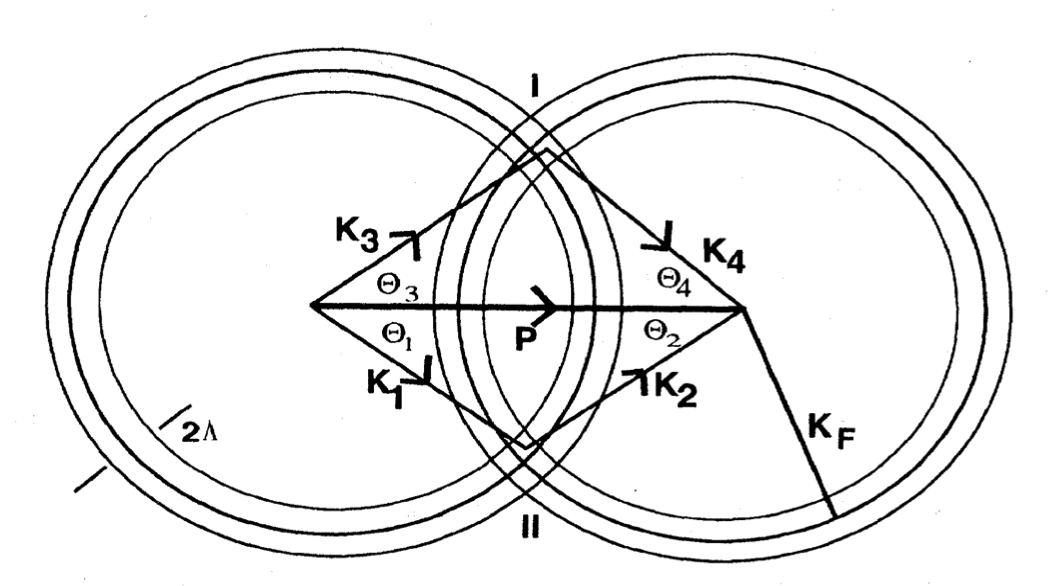
\includegraphics[width=0.5\linewidth]{pics/FL-kcons.png}
	\caption{The geometric construction for determining the allowed values of momenta. If $K_{1}$ and $K_{2}$ add up to $P$, then $K_{3}$ and $K_{4}$ are constrained as shown, if they are to add up to $P$ and lie within the cutoff. If the incoming momenta $K_{1}$ and $K_{2}$ are equal and opposite, the two shells coalesce and $K_{3}$ and $K_{4}$ are free to point in all directions, as long as they are equal and opposite.}
	\label{fig:FL-kcons}
\end{figure}

This equation has only three solutions (see also Fig.~\ref{fig:FL-kcons}):
\begin{equation}
\begin{aligned}
	&\text{Case I:} \quad \bm \Omega_1 = \bm \Omega_3, \\
	&\text{Case II:} \quad \bm \Omega_2 = \bm \Omega_3, \\
	&\text{Case III:} \quad \bm \Omega_1 = -\bm \Omega_2.
\end{aligned}
\end{equation}
Because of the rotational symmetry, the marginal vertex functions are determined solely by two functions:
\begin{eqnarray}
	u[\theta_1,\theta_2,\theta_1,\theta_2] &\equiv& F(\theta_1,\theta_2) = F(\theta_1-\theta_2), \\
	u[\theta_1,\theta_2,\theta_2,\theta_1] &=& -F(\theta_1-\theta_2), \\
	u[\theta_1,-\theta_1,\theta_3,-\theta_3] &\equiv& V(\theta_1,\theta_3) = V(\theta_1-\theta_3).
\end{eqnarray}
Note that the manifestation of the Pauli principle on $F$ and $V$ is somewhat subtle: $F$ will not be antisymmetric under $1 \leftrightarrow 2$ since, according to the way it is defined above, we cannot exchange 1 and 2 without exchanging 3 and 4 at the same time. 
On the other hand, since 3 and 4 can be exchanged without touching 1 and 2 in the definition of $V$, $V$ must go to $-V$ when $1 \leftrightarrow 3$.

\subsection{One-loop RG for 2D System}
We first consider the loop correction to the chemical potential:
\begin{equation}
\begin{aligned}
	\mu^{(2)}(k,\theta,\omega) 
	&= \int_{d\Lambda}\frac{dK'}{2\pi} \int \frac{d\omega'}{2\pi} \int \frac{d\theta'}{2\pi} \frac{F(\theta-\theta')}{i\omega-v_F k'} \\
	&= \int_{-\Lambda}^{-\Lambda+\Lambda dt}\frac{dK'}{2\pi} \int \frac{d\theta'}{2\pi} F(\theta-\theta') \\
	&= \frac{\Lambda}{2\pi} \left[\int\frac{d\phi}{2\pi} F(\phi)\right] dt.
\end{aligned}
\end{equation}
For the vertex correction, again we should consider three channels corresponding to the diagrams:
\begin{equation}
	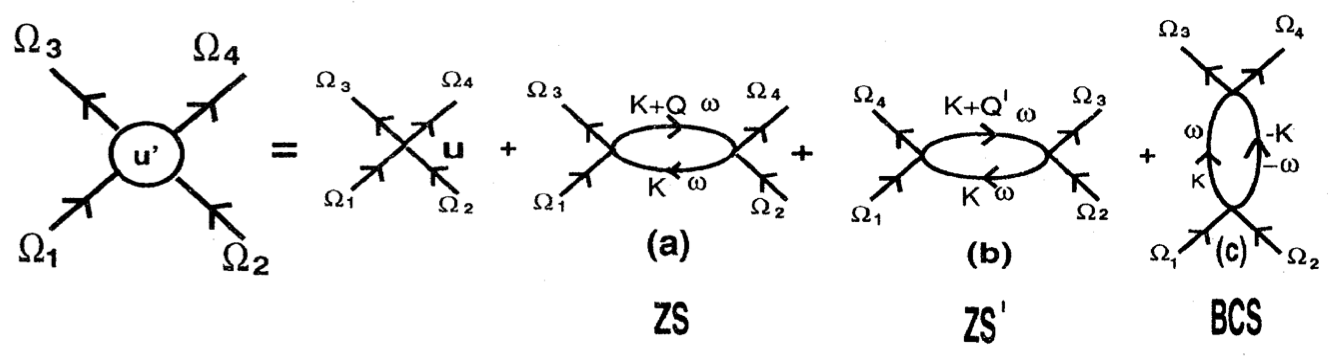
\includegraphics[align=c, width=0.7\linewidth]{pics/FL-4.png}
\end{equation}
First we consider the correction to the $F(\theta)$.
The contribution from the ZS channel (the momentum transfer $Q \simeq 0$) is
\begin{equation}
	F^{(2)}_{\mathrm{ZS}}(\theta_1-\theta_2) = \int_{d\Lambda}\frac{dk}{2\pi}\int \frac{d\omega}{2\pi} \int \frac{d\theta}{2\pi} \frac{F(\theta_1-\theta)F(\theta-\theta_2)}{(i\omega-v_F k)^2}.
\end{equation}
Since two poles of the integrant lie at the same half plane, we can alway choose to close the loop integral along the other half, and thus getting zero contribution.

\begin{figure}[]
	\centering
	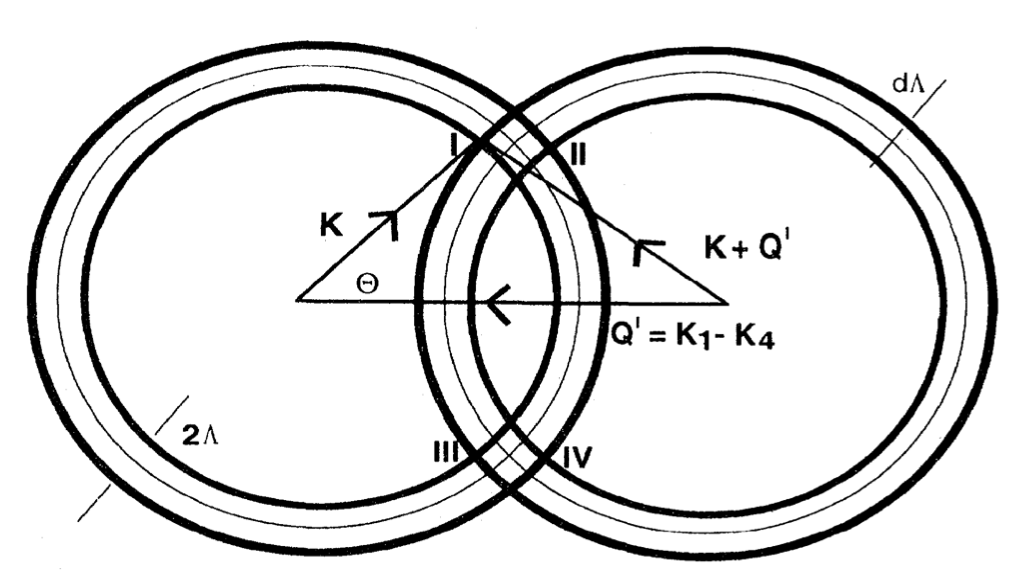
\includegraphics[width=0.4\linewidth]{pics/FL-kshell.png}
	\caption{Construction for determining the allowed values of loop momenta in ZS'. The requirement that the loop momenta come from the shell and differ by $Q'$ forces them to lie in one of the eight intersection regions of width $d\Lambda^2$.}
	\label{fig:FL-kshell}
\end{figure}

For the ZS' channels, the momentum conservation condition (see Fig.~\ref{fig:FL-kshell}) restrict the phase space to be of order $d\Lambda^2$, and thus has no relevant contribution to $F(\theta)$.
Finally, for the same kinematical reason, the BCS diagram does not renormalize $F(\theta)$ at one loop.
Consider Fig.~\ref{fig:FL-kcons}, with $K_3$ and $K_4$ replaced by the two momenta in the BCS loop, $K$ and $P-K$.
In each annulus we keep just two shells of thickness $d\Lambda$ at the cutoff corresponding to the modes to be eliminated. 
The requirement that $K$ and $P-K$ lie in these shells and also add up to $P$ forces them into intersection regions of order $d\Lambda^2$. 
This means the diagram is just as ineffective as the ZS' diagram in causing a flow. 
Thus any $F$ is a fixed point to this order.

Now we consider the correction to the $V(\theta)$ function.
We choose the external momenta equal and opposite and on the Fermi surface. 
The ZS and ZS' diagrams do not contribute to any marginal flow for the same reason that BCS and ZS' did not contribute to the flow of $F(\theta)$.
But the BCS diagram produces a flow:
\begin{equation}
\begin{aligned}
	V^{(2)}_{\mathrm{BCS}}(\theta_1-\theta_3) 
	&= -\frac{1}{2}\int_{d\Lambda}\frac{dk}{2\pi}\int\frac{d\omega}{2\pi}\int\frac{d\theta}{2\pi} 
		\frac{V(\theta_1-\theta)V(\theta-\theta_3)}{(i\omega-v_F k)(-i\omega-v_F k)} \\
	&= -\frac{dt}{4\pi v_F}\int \frac{d\theta}{2\pi}V(\theta_1-\theta)V(\theta-\theta_3).
\end{aligned}
\end{equation} 
We can simplify the picture by going to angular momentum eigenfunctions,
\begin{equation}
	V(\theta) = \sum_l e^{il\theta} V_l,
\end{equation}
which gives the RG flow as
\begin{equation}
	\frac{dV_l}{dt} = -\frac{V_l^2}{4\pi v_F}.
\end{equation}
The solution to the RG flow is:
\begin{equation}
	V_l(t) = \frac{V_l(0)}{1+\frac{V_l(0)}{4\pi v_F}t}.
\end{equation}
What these equations tell us is that if the potential in angular momentum channel $l$ is repulsive, it will get renormalized (logarithmically) down to zero, while if it is attractive, it will run off to large negative values signaling the BCS instability. 
This is the reason the $V$'s are excluded in Landau theory, which assumes we have no phase transitions.\footnote{Remember that the sign of any given $V_l$ is not necessarily equal to that of the microscopic interaction. Kohn and Luttinger have shown (PRL, 15, 524 (1965)) that some of them will be always negative. Thus, the BCS instability is inevitable, though possibly at absurdly low temperatures or absurdly high angular momentum $l$.}




\chapter{One Dimensional Fermi System}

\begin{figure}
	\centering
	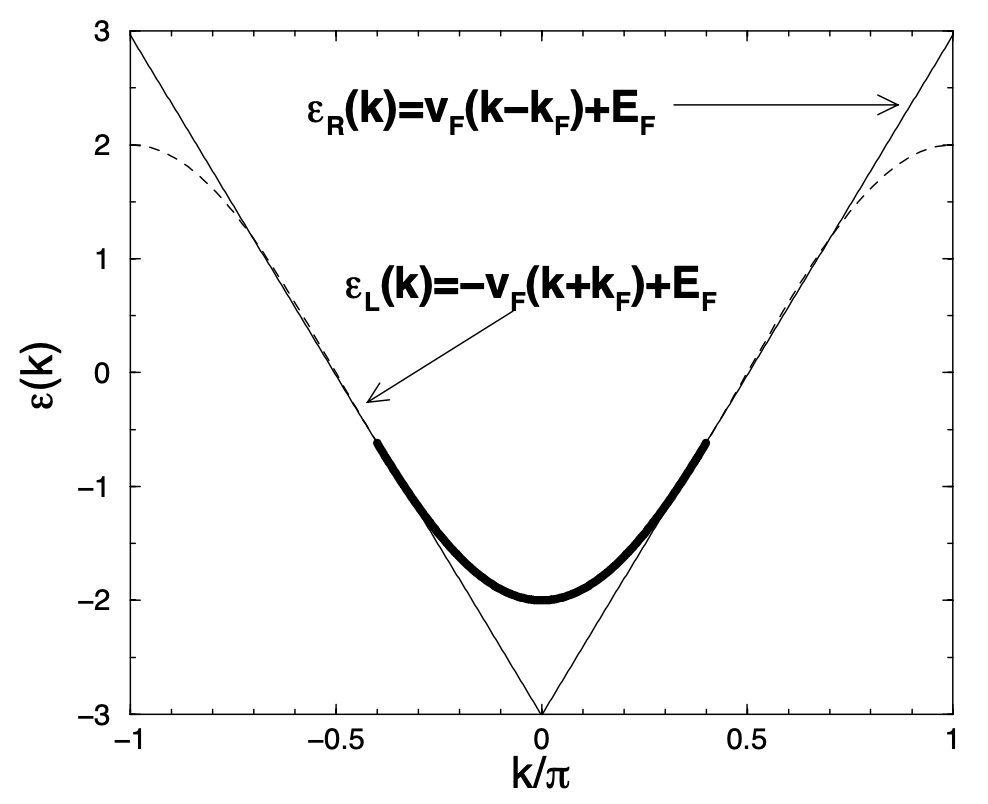
\includegraphics[width=0.4\linewidth]{pics/FL-linearize.png}
	\caption{Linearized Model.}
	\label{fig:bs-linearize}
\end{figure}

In this section, we discuss the one-dimensional interacting Fermi system, described by the Hamiltonian
\begin{equation}
	H = -\frac{1}{2}\sum_{i} (c_i^\dagger c_{i+1} + c_{i+1}^\dagger c_i) + \mu\sum_i c_i^\dagger c_i + \sum_{i,j,k,l} u_{ijkl} c_i^\dagger c_j^\dagger c_k c_l.
\end{equation}
The dispersion for the free theory is $\varepsilon(k) = -\cos k$, near the Fermi surface with momentum $k_F$, the spectrum can be approximately linearized (as shown in Fig.~\ref{fig:bs-linearize}), with the left and right moving fermion modes:
\begin{equation}
	\varepsilon_{R/L}(k) = \begin{cases}
		v_F (k - k_F) & r=R \\
		-v_F (k + k_F) & r=L
	\end{cases},\quad v_F = \sin k_F.
\end{equation}
The fermi momentum is (assume $N_L=N_R$)
\begin{equation}
	k_F = \frac{\pi N}{2L}.
\end{equation}
The state while all fermion modes filled below the Fermi surface and all modes empty above the Fermi surface is defined as the vacuum state $|0\rangle_0$.



\section{Field Theory for Luttinger Liquid}

In this section, we gives a field theoretical analysis of the interacting fermion system in 1D.
For the notational simplicity, we shift the momentum so that
\begin{equation}
	k \rightarrow k' = \begin{cases}
		k - k_F & r=R \\
		-k - k_F & r=L
	\end{cases}.
\end{equation}
The dispersion is then $\varepsilon_r(k) = v_F k$.
In this way, two Fermi points are brought to the origin, the left and right moving branches have the same dispersion.
The integral over momentum shell for both species of fermion can then be denoted by
\begin{equation}
	\int^\Lambda \frac{dK}{2\pi} \equiv \int_{-\Lambda}^\Lambda \frac{dk_L}{2\pi} + \int_{-\Lambda}^\Lambda \frac{dk_R}{2\pi}.
\end{equation}



\subsection{Effective Field Theory}

The effective field theory for the free field is
\begin{equation}
	Z_0 = \prod_{r=L/R}\int D\left[\bar\psi_r(k,\omega),\psi_r(k,\omega)\right] e^{-S_0},
\end{equation}
where the free field action is
\begin{equation}
	S_0 = \sum_{r=L/R} \int^\Lambda_{-\Lambda} \frac{dk}{2\pi} \int^\infty_{-\infty} \frac{d\omega}{2\pi} 
	\bar\psi_r(k,\omega)[-i\omega + v_F k]\psi_r(k,\omega),
\end{equation}
which gives the free field propagator:
\begin{equation}
	G_r(k,\omega) = -\langle \psi_r(k,\omega)\bar\psi_r(k,\omega)\rangle 
	= \frac{1}{i\omega - v_F k}.
\end{equation}
We then consider the rescaling of the cut-off $\Lambda \rightarrow \Lambda/s$. 
To make the free action scale invariant, we define the rescaled variables:
\begin{equation}
	k' = sk, \quad \omega' = s\omega, \quad 
	\psi'_r(k',\omega') = s^{-3/2}\psi_r(k,\omega).
\end{equation}
Then we consider the perturbation from quadratic and quartic terms:
\begin{equation}
\begin{aligned}
	\delta S_2 &= \sum_{r=L/R} \int^\Lambda_{-\Lambda}\frac{dk}{2\pi}\int^\infty_{-\infty} \frac{d\omega}{2\pi} 
	\mu(k,\omega) \bar\psi_r(k,\omega) \psi_r(k,\omega), \\
	\delta S_4 &= \frac{1}{2!2!} \int^\Lambda_{K,\omega} 
	u(4,3,2,1)\bar\psi(4)\bar\psi(3)\psi(2)\psi(1),
\end{aligned}
\end{equation}
where we have suppressed the momentum labels: 
\begin{equation}
	\psi(i) = \psi_{r_i}(k_i,\omega_i), \quad
	u(4,3,2,1) = u(K_4,\omega_4;K_3,\omega_3;K_2,\omega_2;K_1,\omega_1),
\end{equation}
and the integral is defined as:\footnote{The symbol $\bar\delta$ enforces momentum conservation mod $2\pi$, as is appropriate to any lattice problem. A process where lattice momentum is violated in multiples of $2\pi$ is called an \textit{umklapp process}.}
\begin{equation}
\begin{aligned}
	\int_{K \omega}^{\Lambda}
	=& \ \int^\Lambda \frac{d K_1 \cdots d K_4}{(2 \pi)^{4}} \int_{-\infty}^{\infty} \frac{d \omega_{1} \cdots d \omega_{4}}{(2 \pi)^{4}} \times 2 \pi \delta\left(\omega_{1}+\omega_{2}-\omega_{3}-\omega_{4}\right) \\
	&\ \times 2 \pi \bar{\delta}(K_1+K_2-K_3-K_4).
\end{aligned}
\end{equation}
Since this action separates into slow and fast pieces, the effect of mode elimination is simply to reduce $\Lambda$ to $\Lambda/s$ in the integral above. Rescaling moments and fields, we find that
\begin{equation}
	\mu'(k',\omega') = s\cdot\mu\left(\frac{k'}{s}, \frac{\omega}{s}\right).
\end{equation}
Expand $\mu$ in series:
\begin{equation}
	\mu(k, \omega)=\mu_{00}+\mu_{10} k+\mu_{01} i \omega+\cdots+\mu_{n m} k^{n}(i \omega)^{m}+\cdots,
\end{equation}
and compare both sides. The constant piece is a relevant perturbation.
This relevant flow reflects the readjustment of the Fermi sea to a change in chemical potential. 
The correct way to deal with this term is to include it in the free-field action by filling the Fermi sea to a point that takes $\mu_{00}$ into account. 
The next two terms are marginal and modify terms that are already present in the action.

We now turn on the quartic interaction, the dimensional analysis gives the transformation of $u$:
\begin{equation}
	u'_{i_4,i_3,i_2,i_1}(k'_i,\omega'_i) = u_{i_4,i_3,i_2,i_1}\left(\frac{k'_i}{s},\frac{\omega'_i}{s}\right).
\end{equation}
If we expand $u$ in a Taylor series in its arguments and compare coefficients, we find that the constant term u0 is marginal and the higher coefficients are irrelevant. 
Thus, $u$ depends only on its discrete labels and we can limit the problem to just a few coupling constants instead of the coupling function we started with. 
Furthermore, all reduce to just one coupling constant:
\begin{equation}
	u_0 = u_{LRLR} = u_{RLRL} = -u_{RLLR} = -u_{LRRL} \equiv u.
\end{equation}
Other couplings corresponding to the ($LL \rightarrow RR$) process are wiped out by the Pauli principle since they have no momentum dependence and cannot have the desired antisymmetry.

\subsection{RG at One-loop Level}

Consider the infinitesimal rescale $s=e^{dt}$. 
The one-loop contribution to the quadratic term is\footnote{We include an infinitesimal $e^{i\omega\eta}$ to ensure convergence as we do the integral over $\omega$ by closing the upper half-plane.}
\begin{equation}
	\mu^{(2)}_{LL} = 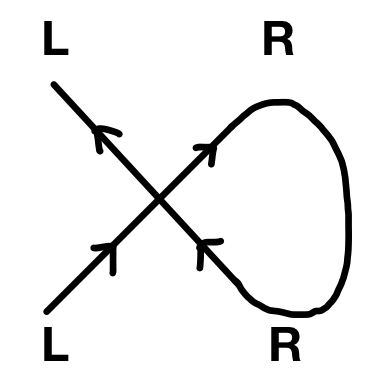
\includegraphics[align=c, width=0.125\linewidth]{pics/FL-1.png}
	= -u \int_{d\Lambda} \frac{dk}{2\pi}\int^\infty_{-\infty}\frac{d\omega}{2\pi}\frac{e^{i\omega \eta}}{i\omega - v_F k},
\end{equation}
where the integral on the momentum shell is
\begin{equation}
	\int_{d\Lambda}\frac{dk}{2\pi} = \int_{-\Lambda}^{-\Lambda(1-dt)} \frac{dk}{2\pi} + \int_{\Lambda(1-dt)}^{\Lambda} \frac{dk}{2\pi}.
\end{equation}
The result gives:
\begin{equation*}
	\mu^{(2)}_{LL}
	= -\frac{u\Lambda}{2 \pi}dt
\end{equation*}
By the symmetry $L \leftrightarrow R$, we know $\mu^{(2)}_{LL}=\mu^{(2)}_{RR}=\mu^{(2)}$, so the RG flow is
\begin{equation}
	\frac{d}{dt}\left[s\cdot\left(\mu+\mu^{(2)}\right)\right] = \mu - \frac{u\Lambda}{2\pi}.
\end{equation}
The one-loop correction to the quartic term ($u_{LRRL}=-u$) have two contributions.
One is called ZS' (zero sound) channel:\footnote{There is actually another zero sound channel ZS, but which has no contribution to the vertex because the diagram contains the vertex of the ($LL \rightarrow RR$) process, which has no relevant contribution the the vertex.}
\begin{equation}
\begin{aligned}
	u^{(2)}_{\mathrm{ZS'}} 
	&= 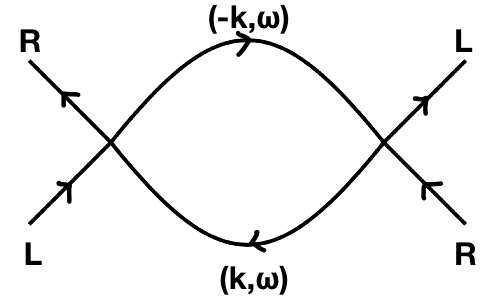
\includegraphics[align=c, width=0.2\linewidth]{pics/FL-2.png} \\
	&= -u^2 \int^\infty_{-\infty}\int_{\Lambda/s<|k|<\Lambda} \frac{d\omega dk}{(2\pi)^2} \frac{e^{i\omega\eta}}{(i\omega+v_F k)(i\omega-v_F k)} \\
	&= u^2\int_{\Lambda/s<|k|<\Lambda} \frac{dk}{2\pi} \frac{1}{2|k|} \\
	&= \frac{u^2}{2\pi}\frac{d\Lambda}{\Lambda}.
\end{aligned}
\end{equation}
The sign is obtained from contracting the Fermion field monomial:
\begin{equation*}
	\wick{
        \c1 {\bar\psi}_L \bar\psi_R \psi_L \c2 \psi_R
        \bar\psi_L \c2 {\bar\psi}_R \c1 {\psi}_L \psi_R
	} = -G_L G_R \bar\psi_R \psi_L \bar\psi_L \psi_R
	= -G_L G_R \bar\psi_L \bar\psi_R \psi_L \psi_R.
\end{equation*}
The other is called the BCS channel:\footnote{The $1/2$ factor comes from the symmetry factor of the diagram.}
\begin{equation}
	u^{(2)}_{\mathrm{BCS}} 
	= 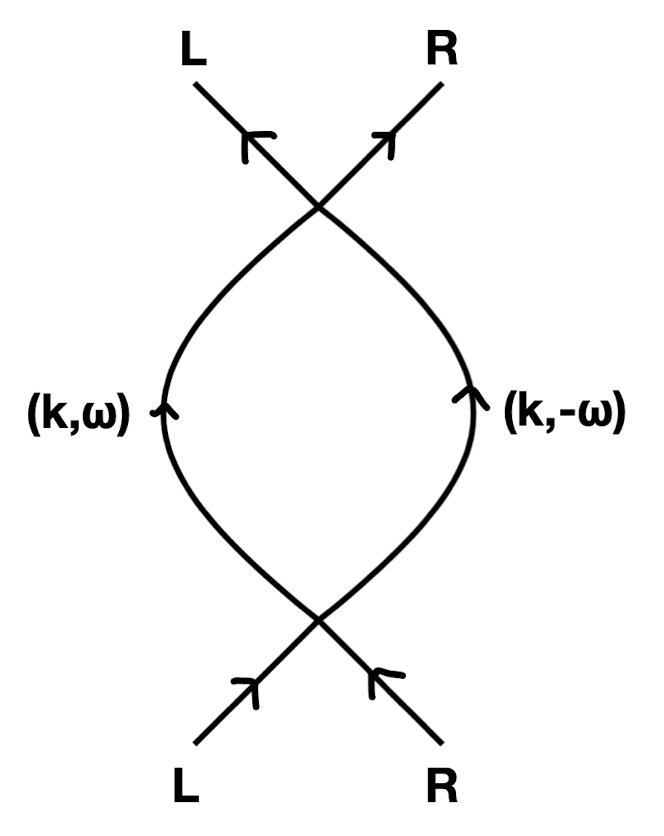
\includegraphics[align=c, width=0.15\linewidth]{pics/FL-3.png} 
	= -\frac{u^2}{2} \sum_{r=L/R}\int^\infty_{-\infty}\int_{d\Lambda} \frac{d\omega dk_i}{(2\pi)^2} \frac{e^{i\omega\eta}}{(i\omega-v_F k)(-i\omega-v_F k)}.
\end{equation}
The sign is obtained from the contraction:
\begin{equation*}
	\wick{
        \bar\psi_L \bar\psi_R \c1 \psi_L \c2 \psi_R
        \c1 {\bar\psi}_L \c2 {\bar\psi}_R \psi_L \psi_R
	} = -G_L G_R \bar\psi_L \bar\psi_R \psi_L \psi_R.
\end{equation*}
Note that we will obtained a factor of 2 since in this channel, the intermedia propagator can be left mover or right mover.
We see that two contributions cancel out:
\begin{equation}
	u^{(2)}_{\mathrm{ZS'}} + u^{(2)}_{\mathrm{BCS}} = 0.
\end{equation}
Together, the RG flow to the one-loop level is
\begin{equation}
	\frac{d\mu}{dt} = \mu - \frac{u\Lambda}{2\pi}, \quad
	\frac{du}{dt} = 0.
\end{equation}
The fixed point solution to the RG flow is:
\begin{equation}
	\mu^* = \frac{u^*\Lambda}{2\pi},
\end{equation}
where the fixed-point value of $u^*$ is arbitrary. 
The vanishing beta function predict that the ground state of one-dimensional weakly interacting Fermi gas remains gapless (rather than develops CDW order and becomes gapped).


\section{Bosonization}


In this section, we map the 1D interacting fermion system to a bosonic one.
From the RG analysis, we know that the low energy excitations are particle-hole modes:
\begin{equation}
	\rho_{k}^\dagger = \sum_{q} c_{q+k}^\dagger c_{q}, \quad
	\rho_{k} = \sum_{q} c_{q}^\dagger c_{q+k} = \rho_{-k}^\dagger.
\end{equation}

In the following, we restore the notation for the momentum (i.e., use the original momentum instead of the shifted one).
 

\subsection{Bosonic Hilbert Space}
To simplify the discussion, here we consider only a single branch of Fermion, as depicted in Fig.~\ref{fig:bs-hilbert}. The generalization to multiple branches is trivial since the dispersion is the same.

\begin{figure}
	\centering
	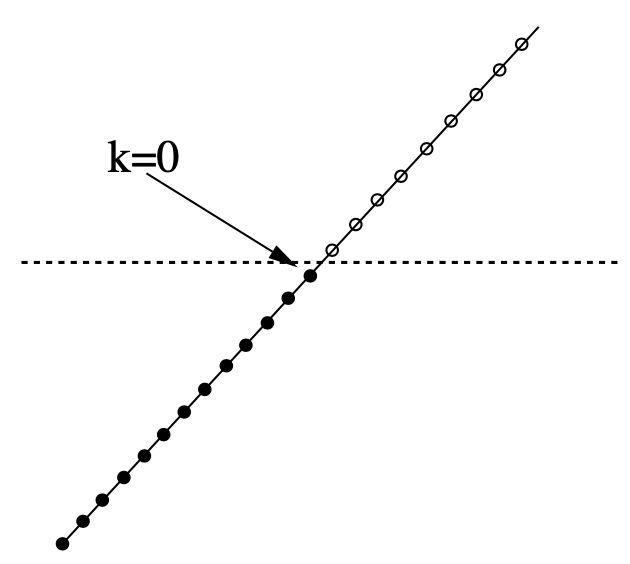
\includegraphics[width=0.25\linewidth]{pics/FL-hilbert.png}
	\caption{The vacuum state $|0\rangle_0$ of a single fermion branch.}
	\label{fig:bs-hilbert}
\end{figure}

The commutation relation between $\rho_k$ and $\rho_{k'}^\dagger$ is:\footnote{We use the identity $[AB,C] = A[B,C] + [A,C]B$ and $[A,BC]=\{A,B\}C - B\{A,C\}$.}
\begin{equation}
\begin{aligned}
	\left[\rho_{k}, \rho_{k'}^\dagger \right]
	&= \sum_{q_1, q_2} \left[c_{q_1}^\dagger c_{q_1+k}, c_{q_2+k'}^\dagger c_{q_2}\right] \\
	&= \sum_{q_1, q_2} \left\{c_{q_1}^\dagger \left[c_{q_1+k}, c_{q_2+k'}^\dagger c_{q_2}\right] +\left[c_{q_1}^\dagger, c_{q_2+k'}^\dagger c_{q_2}\right] c_{q_1+k}\right\} \\
	&= \sum_{q_1, q_2} \left\{ \delta_{q_1+k,q_2+k'} c_{q_1}^\dagger c_{q_2} -
		\delta_{q_1,q_2} c_{q_2+k'}^\dagger c_{q_1+k} \right\} \\
	&= \sum_{q}\left[c^\dagger_{q+k'-k} c_{q}-c^\dagger_{q+k'} c_{q+k}\right].
\end{aligned}
\end{equation}
For $k \ne k'$, it is clear that $[\rho_{k},\rho_{k'}^\dagger]=0$.
However, when $k = k'$, we should be careful about the subtraction, since it evolve two infinities of which the subtraction is ill-defined.

Here we deal with the infinity with the lattice regularization, i.e., we think of the linearized theory as the low-energy approximation of a lattice mode, where the dispersion form a single energy band.
The left/right movers are actually in a single band but with positive/negative momentum.
Consider for example the density operator for the right mover, the commutator of the right moving density operator is then
\begin{equation}
	\left[\rho_{k,r}, \rho_{k,r}^\dagger \right] = \sum_{0<q<\pi} [n_{q,r}-n_{k+q,r}].
\end{equation}

\begin{figure}
	\centering
	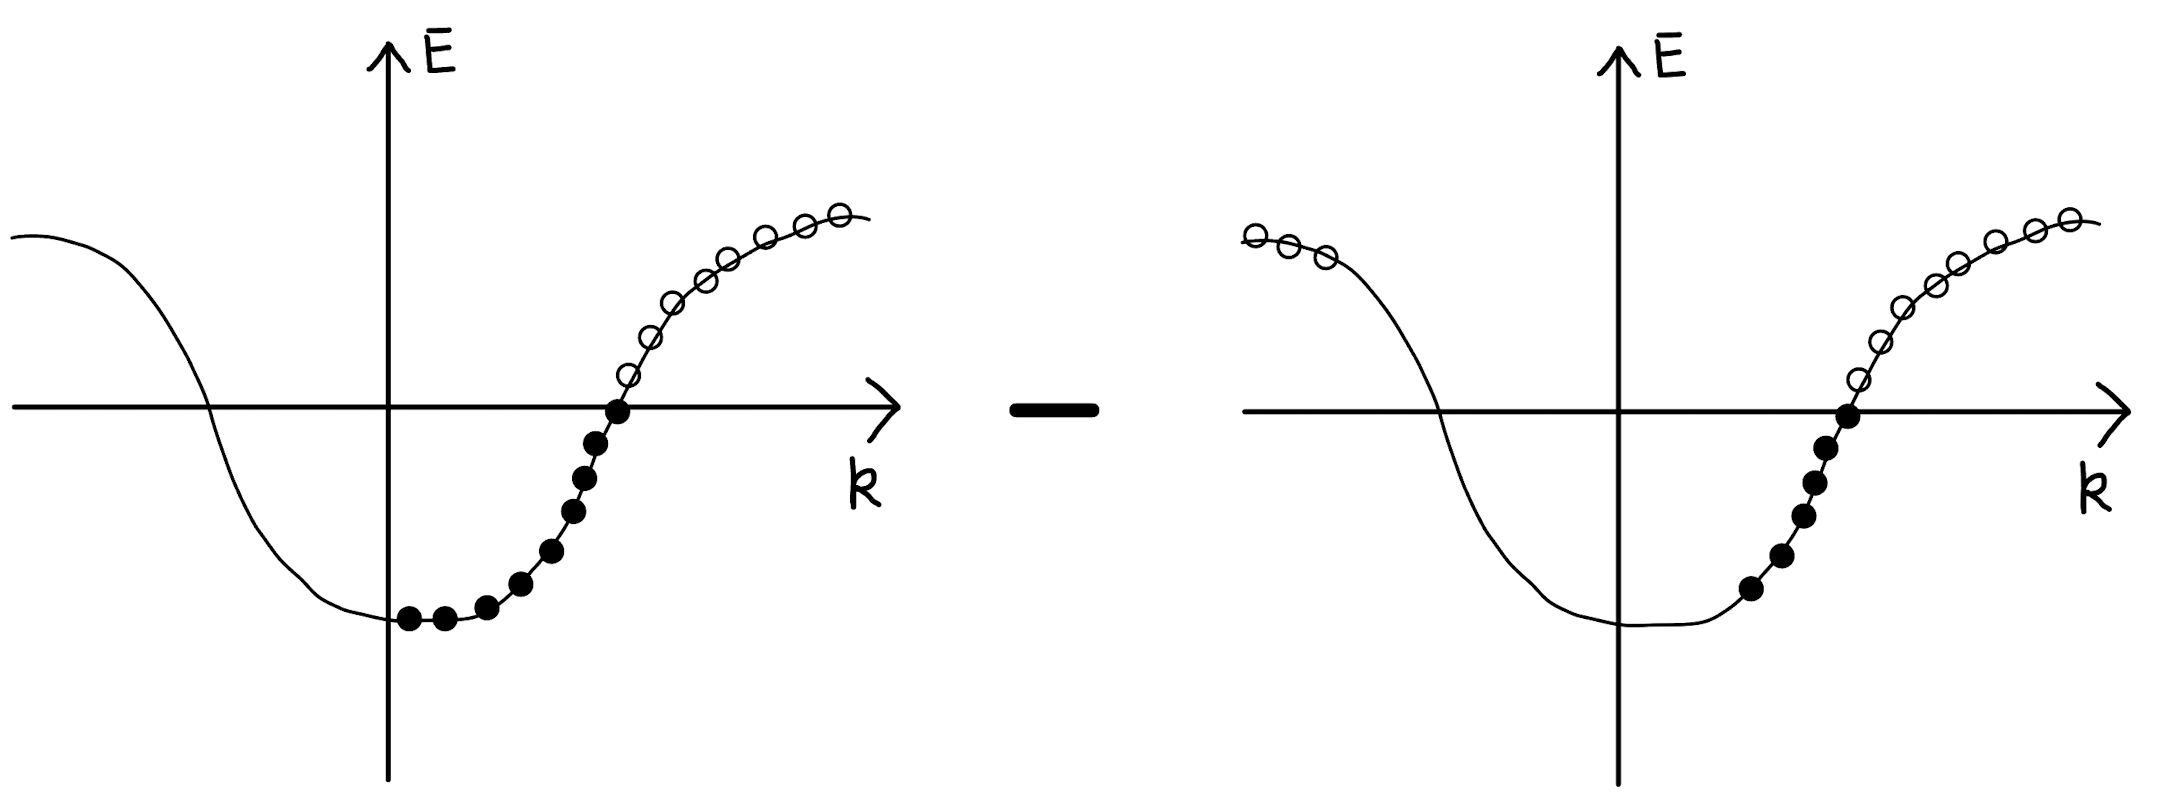
\includegraphics[width=0.6\linewidth]{pics/BS-k-shift}
	\caption{Shift of the right-moving modes.}
	\label{fig:bs-k-shift}
\end{figure}

Consider for example the case where $r=R,k>0$, as shown in Fig.~\ref{fig:bs-k-shift}.
The subtraction result in a sum of low-lying right-mover number operator minus a sum of high-energy left-mover number operator, which behaves like a constant in the low energy regime. 
The above analysis gives the commutation relation:
\begin{equation}
	\left[\rho_{k,r}, \rho_{kr}^\dagger \right] \simeq \frac{qL}{2\pi} \equiv n_q.
\end{equation}

\begin{framedrmk}[Normal Ordering]
Field theoretically, we can also evaluate the infinite subtraction by the normal-order expression:
\begin{equation}
	O = {:\mathrel{O}:} + \langle 0|O|0\rangle.
\end{equation}
For $k\ne k'$, since $\langle 0|c_k^\dagger c_k|0\rangle=0$, the normal ordering does not affect the result, while for the $k=k'$ case, the normal ordering takes care of the infinity of the particle number operator:
\begin{equation}
\begin{aligned}
	\sum_q [n_{q} - n_{q+k}]
	&= \sum_q \left[{:\mathrel{n_{q}}:} - {:\mathrel{n_{q+k}}:} 
		+ \langle0|n_{q}|0\rangle -\langle0|n_{q+k}|0\rangle \right] \\
	&= \sum_q [\langle0|n_{q}|0\rangle -\langle0|n_{q+k}|0\rangle].
\end{aligned}
\end{equation}
The final result gives the same result as the above discussions.
\end{framedrmk}

We denote the ground state with $N$ fermions as $|N\rangle_0$, which satisfies:
\begin{equation}
	\rho_{p>0}|N\rangle_0 = \rho^\dagger_{p<0}|N\rangle_0 = 0.
\end{equation}
We can thus define a set of canonical bosonic modes:
\begin{equation}
	b_p^\dagger = i\frac{\rho^\dagger_p}{\sqrt{n_p}}, \quad 
	b_p = -i\frac{\rho_p}{\sqrt{n_p}}, \quad [b_q,b_{q'}^\dagger] = \delta_{qq'}.
\end{equation}
We will assume $p>0$, and the $\pm i$ factor is a convention chosen for the future convenience.

Now we discuss the construction of the Hilbert space using the bosonic modes.
The $N$-particle sector is spanned by the states generated by applying $b_q^\dagger$'s to the ground state $|N\rangle_0$.
A general $N$-particle state has the form:
\begin{equation}
	|N\rangle = f(\{b_q^\dagger\})|N\rangle_0.
\end{equation}
Note that the bosonic mode $b_q$ does not change the particle number:\footnote{The particle number operator is defined by the normal order expression $\hat{N} = \sum_k {:\mathrel{c_{k}^\dagger c_{k}}:}$.}
\begin{equation}
	\left[\hat N, b_q \right] = \left[\hat N, b_q^\dagger \right] = 0.
\end{equation}
In order to construct the full Fock space, we also need to include a particle-number-changing operator, the \textit{Klein factor} $\hat F$, that shifts the total number of fermion by one, and commutes with bosonic operator $b_q$:
\begin{equation}
	\left[\hat F, b_q \right] = \left[\hat F, b_q^\dagger \right] = 0, \quad
	\left[\hat F, \hat N \right] = \hat F, \quad 
	\left[\hat F^\dagger, \hat N \right] = -\hat F^\dagger.
\end{equation}
For system with different fermion species (labeled by $\eta$), the set of operator
\begin{equation*}
	\{b_{q,\eta}, b_{q,\eta}^\dagger, \hat F_\eta, \hat N_\eta\}
\end{equation*}
form a complete operator basis for the Hilbert space within the low-energy regime.
However, note that the Klein factor also takes care of the fermionic statistics. 
That is, for the state denoted as
\begin{equation}
	|\{N_i\}\rangle = |N_1,N_2,\cdots,N_m\rangle
\end{equation}
The Klein factor $\hat F_\eta$ acting on the state will contribute an additional factor
\begin{equation}
	\hat F_\eta|\{N_i\}\rangle = \exp\left(i\pi\sum_{j=1}^{\eta-1}N_j\right)|N_1,\cdots,N_\eta-1,\cdots,N_m\rangle.
\end{equation}

\subsection{Bosonization of Fermion Field}
Now we try to express the fermion operator 
\begin{equation}
	\psi(x) = \frac{1}{\sqrt{L}} \sum_p e^{ipx} c_{p}
\end{equation}
by the bosonic operator set.
First we consider the commutation relation between the fermion field operator and bosonic mode:
\begin{equation}\label{eq:bs-comm-1}
\begin{aligned}
	\left[b_q,\psi(x)\right] &= \frac{1}{\sqrt L}\frac{i}{\sqrt{n_q}}\sum_{k}\sum_{p} e^{ipx} [c^\dagger_{k}c_{k+q,r'},c_{p}] \\
	&= -\frac{1}{\sqrt L} \frac{i}{\sqrt{n_q}} \sum_{p} e^{ipx} c_{p+q} 
	= -i\frac{1}{\sqrt{n_q}} e^{-iqx} \psi(x).
\end{aligned}
\end{equation}
Similarly,
\begin{equation}\label{eq:bs-comm-2}
	\left[b_q^\dagger,\psi(x)\right] = i\frac{e^{iqx}}{\sqrt{n_q}} \psi(x).
\end{equation}
For future convenience, we define a c-number factor:
\begin{equation}
	\alpha_q(x) \equiv \frac{1}{\sqrt{n_q}} e^{iqx},\quad
	[b_q^\dagger,\psi(x)] = i\alpha_q(x) \psi(x),\quad
	[b_q,\psi(x)] = -i \alpha^*_q(x) \psi(x).
\end{equation}
Since $b_q|N\rangle_0 = 0$, the commutation relation (\ref{eq:bs-comm-1}) leads to
\begin{equation}
	\left[b_{q}, \psi(x)\right]|N\rangle_{0} 
	=b_{q} \psi(x)|N\rangle_{0} 
	= -i\alpha_q^*(x) \psi(x)|N\rangle_{0}.
\end{equation}
Thus, $\psi(x)|N\rangle_0$ is an eigenstate of $b_q$, i.e., a coherent state:
\begin{equation}
	\psi(x)|N\rangle_0 
	= \Lambda(x) \hat F \exp\left[-i\sum_{q>0} \alpha_q^*(x) b_q^\dagger\right]|N\rangle_0
\end{equation}
where $\Lambda(x)$ is a c-number, which can be determined by
\begin{equation*}
	{}_{0}\langle N-1|\psi(x)| N\rangle_{0}=\Lambda(x)\ {}_{0}\langle N|\exp \left[-i\sum_{q>0} \alpha^*_q(x) b_{q}^{\dagger}\right]| N\rangle_{0} = \Lambda(x).
\end{equation*}
The left-hand side can be computed directly, the result is\footnote{Note that the Fermi point locates at $k_F=\frac{2\pi N}{L}$.}
\begin{equation}
	\Lambda(x) = \frac{1}{\sqrt L}\sum_k e^{ikx}\ {}_{0}\langle N-1| c_{k,r}|N\rangle_0 
	= \frac{1}{\sqrt L} e^{i\frac{2\pi N}{L}},
\end{equation}
In this way, we get
\begin{equation}
	\psi(x)|N\rangle_{0} = \frac{\hat F}{\sqrt{L}} e^{i \frac{2 \pi \hat{N} x}{L}} \exp \left[-i\sum_{q>0} \alpha^*_q(x) b_{q}^{\dagger}\right]|N\rangle_{0}
\end{equation}
The commutation relation (\ref{eq:bs-comm-2}) also leads to:\footnote{We denote $\alpha_q(x) \equiv e^{iqx}/\sqrt{n_q}$ to simplify the notation.}
\begin{equation*}
\begin{aligned}
	\psi(x) b_{q}^{\dagger} 
	&=\left[b_{q}^{\dagger}-i\alpha_{q}(x)\right] \psi(x) \\
	\Rightarrow \psi(x)\left(b_{q}^{\dagger}\right)^{n} 
	&=\left[b_{q}^{\dagger}-i\alpha_{q}(x)\right]^{n} \psi(x) \\
	\Rightarrow \psi(x) f\left[\left\{b_{q}^{\dagger}\right\}\right] 
	&=f\left[\left\{b_{q}^{\dagger}-i\alpha_{q}(x)\right\}\right] \psi(x).
\end{aligned}
\end{equation*}
Then, for a generic $N$-particle state:
\begin{equation}\label{eq:bs-temp1}
\begin{aligned}
	\psi(x)|N\rangle 
	&=f\left[\left\{b_{q}^{\dagger}-i\alpha_{q}(x)\right\}\right] \psi(x)|N\rangle_{0} \\
	&=f\left[\left\{b_{q}^{\dagger}-i\alpha_{q}(x)\right\}\right] \frac{\hat{F}}{\sqrt{L}} e^{i \frac{2 \pi \hat{N} x}{L}} \exp \left[-i\sum_{q>0} \alpha^*_{q}(x) b_{q}^{\dagger}\right]|N\rangle_{0} \\
	&=\frac{\hat{F}}{\sqrt{L}} e^{i \frac{2 \pi \hat{N} x}{L}} \exp \left[-i\sum_{q>0} \alpha^*_{q}(x) b_{q}^{\dagger}\right] f\left[\left\{b_{q}^{\dagger}-\alpha_{q}(x)\right\}\right]|N\rangle_{0}.
\end{aligned}
\end{equation}
Using the BCH formula
\begin{equation}
	e^A B e^{-A} = e^{[A,\cdot]} B = B + [A,B] + \frac{1}{2!}[A,[A,B]]+\cdots,
\end{equation}
we have the identity:
\begin{equation*}
\begin{aligned}
	\exp \left[-i\sum_{q>0} \alpha_{q}(x) b_{q}\right] b_{q}^{\dagger} \exp \left[i\sum_{q>0} \alpha_{q}(x) b_{q}\right] &=b_{q}^{\dagger}-i\alpha_{q}(x) \\
	\Rightarrow \exp \left[-i\sum_{q>0} \alpha_{q}(x) b_{q}\right] f\left[b_{q}^{\dagger}\right] \exp \left[i\sum_{q>0} \alpha_{q}(x) b_{q}\right] &=f\left[\left\{b_{q}^{\dagger}-i\alpha_{q}(x)\right\}\right].
\end{aligned}
\end{equation*}
Eq.~(\ref{eq:bs-temp1}) can be further simplified to:
\begin{equation*}
\begin{aligned}
	\psi(x)|N\rangle 
	=&\ \frac{\hat{F}}{\sqrt{L}} e^{i \frac{2 \pi \hat{N} x}{L}} e^{-i\sum_{q>0} \alpha^*_{q}(x) b_{q}^{\dagger}} e^{-i\sum_{q>0} \alpha_{q}(x) b_{q}} f\left[b_{q}^{\dagger}\right] e^{i\sum_{q>0} \alpha_{q}(x) b_{q}} |N\rangle_{0} \\
	=&\ \frac{\hat{F}}{\sqrt{L}} e^{i \frac{2 \pi \hat{N} x}{L}} \exp \left[-i\sum_{q>0} \alpha^*_{q}(x) b_{q}^{\dagger}\right] \exp \left[-i\sum_{q>0} \alpha_{q}(x) b_{q}\right]|N\rangle.
\end{aligned}
\end{equation*}
We thus express the Fermi field operator in bosonic operator:
\begin{equation}\label{eq:bs-fermi-field-1}
	\psi(x) = \frac{\hat{F}}{\sqrt{L}} e^{i \frac{2 \pi \hat{N} x}{L}} e^{-i\sqrt{2\pi}\varphi^\dagger(x)} e^{-i\sqrt{2\pi}\varphi(x)},
\end{equation}
where we have introduced a bosonic field:\footnote{The ``converging factor'' $e^{-a q / 2}$ is important in defining a proper bosonic theory in 1D. These equations should always be viewed as having $e^{-a q / 2}$ to ensure convergence at intermediate steps, but final results should be written taking $a \rightarrow 0^{+}$.}
\begin{equation}
	\varphi(x) = \frac{1}{\sqrt{2\pi}}\sum_{q>0} e^{-a q/2} a_{q}(x) b_{q}.
\end{equation}
Now we introducing the bosonic field:
\begin{equation}
	\phi(x) \equiv \varphi(x)+\varphi^{\dagger}(x)
	= \frac{1}{\sqrt{2\pi}} \sum_{q>0} \frac{e^{-a q/2}}{\sqrt{n_q}} \left[e^{i q x} b_{q}+e^{-i q x} b_{q}^{\dagger}\right].
\end{equation}
We can expressed the fermion field as:\footnote{We use the identity $e^A e^B = e^{A+B}e^{\frac{1}{2}[A,B]}$ if both $A$ and $B$ commutes with $[A,B]$.}
\begin{equation*}
	\psi(x) = \frac{\hat{F}}{\sqrt{L}} e^{i\frac{2\pi \hat N x}{L}} e^{-i\sqrt{2\pi}\phi(x)}
	e^{\pi[\varphi(x),\varphi^\dagger(x)]}.
\end{equation*}
The commutation relation between $\varphi$ and $\varphi^\dagger$ is
\begin{equation*}
	\left[\varphi(x),\varphi^\dagger(y)\right]
	= \frac{1}{L} \sum_q \frac{e^{iq(x-y+ia)}}{q} 
	= -\frac{1}{2\pi}\ln\left\{ 1-\exp\left[\frac{2\pi i}{L}(x-y+ia)\right]\right\}.
\end{equation*}
Set $x=y$, take limit $a\rightarrow 0^+$,
\begin{equation*}
	\exp\left\{\pi[\varphi(x),\varphi^\dagger(x)] \right\} = \lim_{a\rightarrow0^+} \left[1-\exp\left(-\frac{2\pi a}{L}\right)\right]^{-\frac{1}{2}}
	\rightarrow \sqrt{\frac{L}{2\pi a}}.
\end{equation*}
so we have
\begin{equation}\label{eq:bs-fermi-field}
	\psi(x) = \frac{\hat{F}}{\sqrt{2\pi a}}e^{i\frac{2\pi\hat N x}{L}}e^{-i\sqrt{2\pi}\phi(x)}.
\end{equation}
The divergent factor $1/\sqrt{2\pi a}$ appears because Eq.~(\ref{eq:bs-fermi-field}) is not normal-ordered.
We can check the result by normal-ordering the bilinear term $\psi^\dagger(x+a)\psi(x)$.
Insert Eq.~(\ref{eq:bs-fermi-field}) into the expression, we have:
\begin{equation}
	\psi^\dagger(x+a)\psi(x)
	\simeq \frac{e^{-i\frac{2\pi\hat N a}{L}}}{2\pi a}
	e^{i\sqrt{2\pi}\partial_x\phi(x)  a} 
	e^{\pi[\phi(x+ a),\phi(x)]}.
\end{equation}
The commutation relation is:
\begin{equation}
\begin{aligned}
	\left[\phi(x),\phi(y)\right] 
	&= -\frac{1}{2\pi}\ln \left\{\frac{1-\exp \left[\frac{2 \pi i}{L}(x-y+i  a)\right]}{1-\exp \left[-\frac{2 \pi i}{L}(x-y-i  a)\right]}\right\} \\
	&\stackrel{ a \rightarrow 0}{\longrightarrow} 
		\frac{i}{2} \operatorname{sgn}(x-y)-\frac{i}{L}(x-y).
\end{aligned}
\end{equation}
To the lowest order of $a/L$: 
\begin{equation}
	\psi^\dagger(x+a)\psi(x) \simeq \frac{i}{2\pi a} + \frac{\hat N+1}{L} - \frac{1}{\sqrt{2\pi}}\partial_x\phi(x).
\end{equation}
The normal ordering will delaminate all constant, including the divergent one:
\begin{equation}
	{:\mathrel{\psi^\dagger(x+a)\psi(x)}:}
	= \frac{\hat N}{L} - \frac{1}{\sqrt{2\pi}}\partial_x\phi(x).
\end{equation}
We will show in the following the above equation agrees with the bosonization of fermion bilinear $\psi^\dagger(x)\psi(x)$ term.




\subsection{Bosonization Dictionary}
Now we are going to establish a bosonization dictionary.
To tell the complete story, we are now working for both the right-moving and left-moving fermion branches.
In this case, we express the fermion as a spinor:
\begin{equation}
	\psi = \left(\begin{array}{c}
		\psi_L \\ \psi_R
	\end{array} \right),\quad
	\bar\psi = \psi^\dagger\sigma^x =  \left(\begin{array}{cc}
		\psi^\dagger_R & \psi_L^\dagger
	\end{array} \right).
\end{equation}
We also define a new set of bosonic fields
\begin{equation}
	\phi(x) \equiv \phi_R(x) + \phi_L(x), \quad
	\theta(x) \equiv \phi_R(x) - \phi_L(x).
\end{equation}
First we consider the fermion bilinear (for $r=L/R$):
\begin{equation}
\begin{aligned}
	{:\mathrel{\psi_r^\dagger(x)\psi_r(x)}:}
	&= \frac{1}{L}\sum_{q} {:\mathrel{c_{q,r}^\dagger c_{q,r}}:} + \frac{1}{L}\sum_{q>0}[e^{-iqx}\rho^\dagger_{q,r}+e^{iqx}\rho_{q,r}] \\
	&= \frac{\hat N_r}{L} - \frac{1}{2\pi} \sum_{q>0} \frac{iq}{\sqrt{n_q}} \left[e^{iqx}b_{q,r} - e^{-iqx}b^\dagger_{q,r}\right].
\end{aligned}
\end{equation}
We then get:
\begin{equation}
	{:\mathrel{\psi^\dagger(x)\psi(x)}:}
	= \frac{\hat N_L +\hat N_R}{L} - \frac{1}{\sqrt{2\pi}} \partial_x \left[\phi_L(x)+\phi_R(x)\right].
\end{equation}



Now we go back to the Hamiltonian with linear dispersion (for single fermion branch):
\begin{equation}
	H_0 = v_F \sum_{k,r} k\ {:\mathrel{c_{k,r}^\dagger c_{k,r}}:} 
	= v_F \int dx\ {:\mathrel{\psi^\dagger(x)(-i\partial_x)\psi(x)}:}.
\end{equation}
Since $b_q^\dagger$ raise the energy of any eigenstate of $H_0$ by $q$ unit, we have the commutation relation:
\begin{equation}
	\left[H_0,b_{q,r}^\dagger\right] = q b_{q,r}^\dagger.
\end{equation}
The Hamiltonian satisfies such relation can only be the bosonic bilinear:
\begin{equation}
	H_0 = v_F \sum_{r}\sum_{q>0} q b_{q,r}^\dagger b_{q,r} + \frac{\pi v_F}{L} \sum_r \hat{N}_r(\hat{N}_r+1).
\end{equation}
The constant part comes from the fact that
\begin{equation*}
	H_0|N\rangle_0 = \frac{2\pi v_F}{L} \frac{\sum_r\hat{N}_r(\hat{N}_r+1)}{2}|N\rangle_0, \quad
	b_{q,r}^\dagger b_{q,r} |N\rangle_0 = 0.
\end{equation*}
Also, the bosonic operator can also be expressed as
\begin{equation}
	H_0 = \frac{v_F}{2} \int dx\ {:\mathrel{[\partial_x \phi(x)]^2}:} + \frac{\pi v_F}{L}\sum_r \hat{N}_r(\hat{N}_r+1).
\end{equation}






\chapter{Topological Field Theory}

\section{Chern-Simons Theory}
Assume the action of the microscopical theory has the form $S[\psi_i]$, where $\{\psi_i\}$ denotes all degrees of microscopical freedom.
If the system has the U(1) symmetry, we can always rewrite the field theory as a gauge theory:
\begin{equation}
	S[\psi_i; A] = S[\psi_i] + \int d^dx\ j^\mu(x) A_\mu(x),
\end{equation}
where the current $j^\mu$ is the Noether current.
The gauge field $A^\mu(x)$ is regarded as the back ground field which has no dynamics.
If we are interested in the low-energy physics, especially for gapped system, the ground state physics, we can formally integrate out other degrees of freedom, the resulting effective theory has only the gauge degree of freedom:
\begin{equation}
	Z_{\mathrm{eff}}[A] = \int D[\psi_i] e^{i S[\psi_i;A]}.
\end{equation}
In this section, we consider the effective gauge field on $(2+1)$-dimensional space-time.
The effective action should also be gauge-invariant.
The allowed terms include
\begin{equation*}
	A \wedge dA,\ dA \wedge dA,\ \text{higher order terms}.
\end{equation*}
From dimensional analysis, the first term is most relevant in the low-energy.
Such effective theory is the \textit{Chern-Simons theory}:
\begin{equation}
	S_{\mathrm{CS}} = \frac{k}{4\pi}\int d^3 x\ \varepsilon_{\mu\nu\rho} A^\mu \partial^\nu A^\rho.
\end{equation}


    
\end{document}
